\chapter{Hydrocarbons}

\section{Carbon-Carbon Single Bonds}

\subsection{Ethane}

We saw in Chapter 9, that the ground state of CH$_3$, methyl radical, 
is planar with a singly occupied $p$ orbital perpendicular to the plane
\begin{equation}
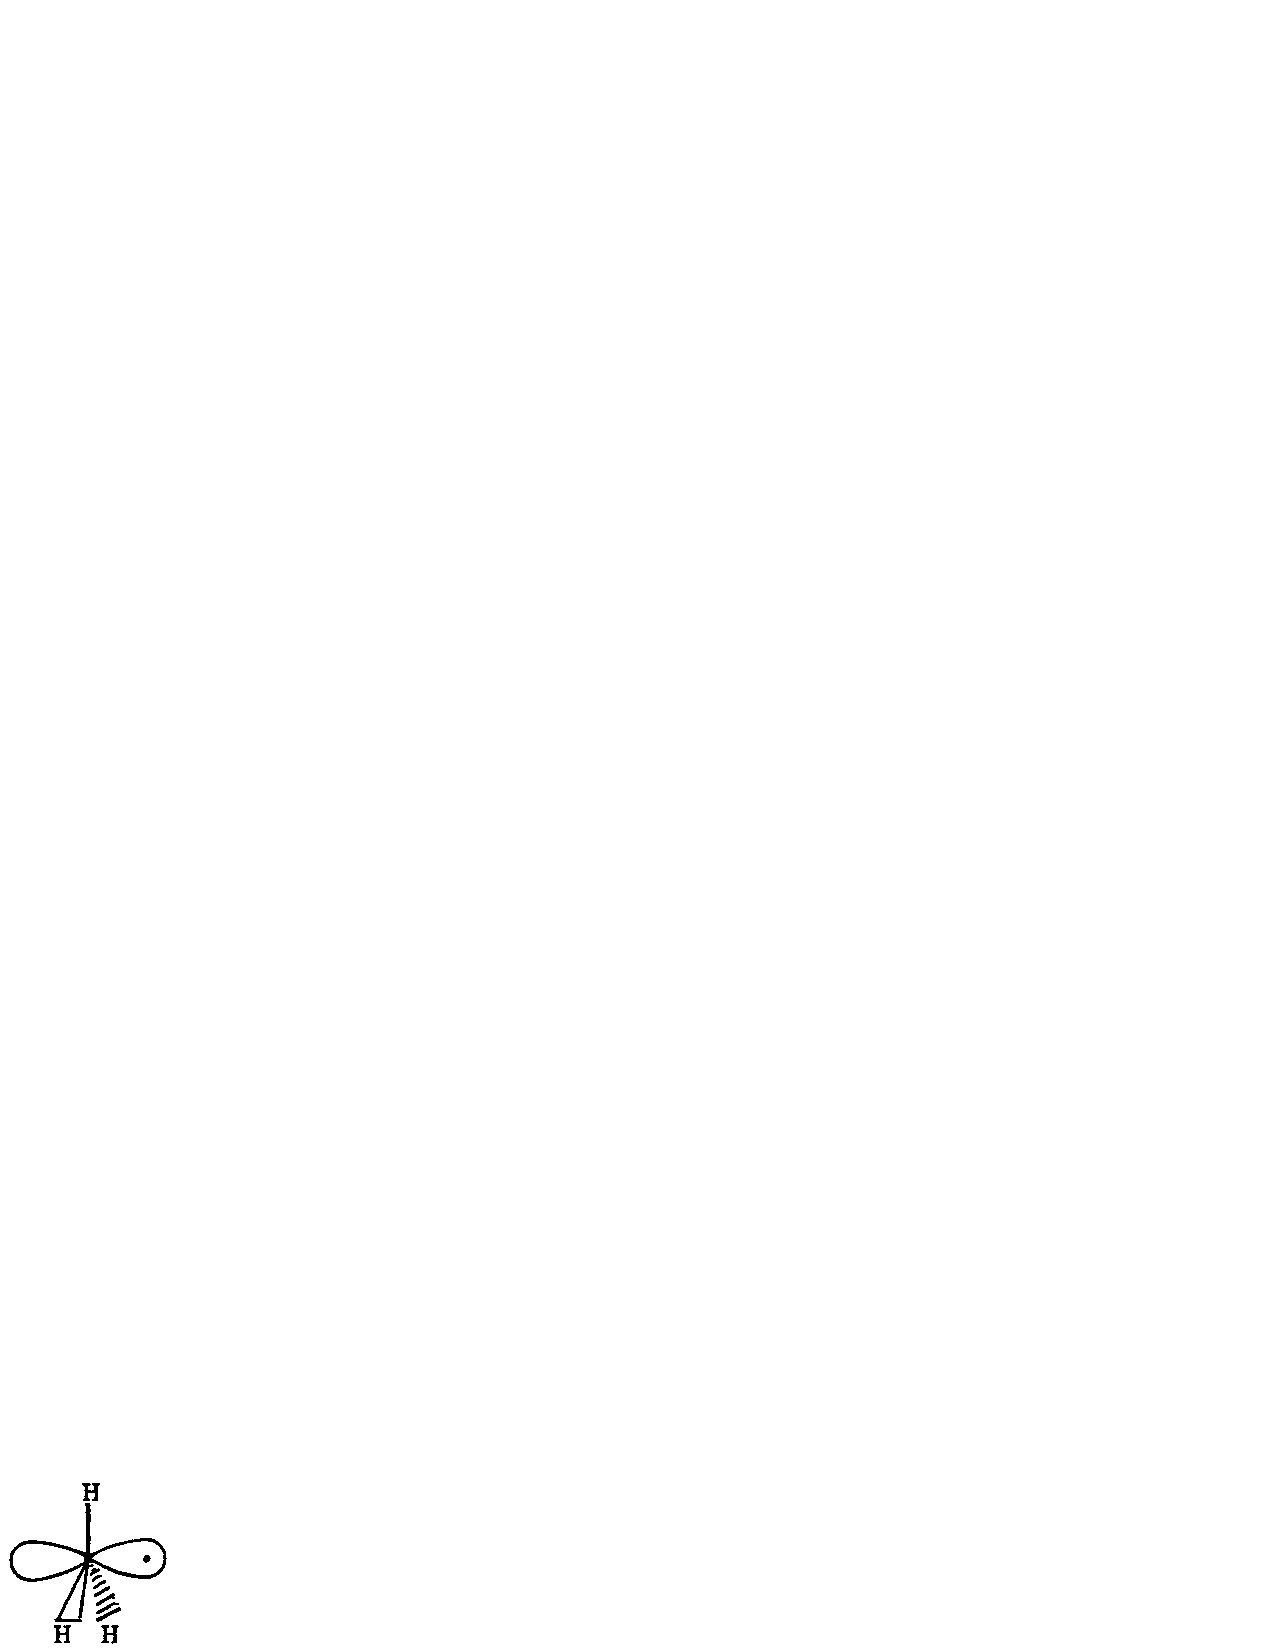
\includegraphics{fg7a}
\label{chap7-eqno1}
\end{equation}
and we found that bonding an H to CH$_3$ leads to a tetrahedral 
molecule, 109.5$^{\circ}$ bond angle.  Now, consider bonding two methyl 
radicals together to form ethane
\begin{equation}
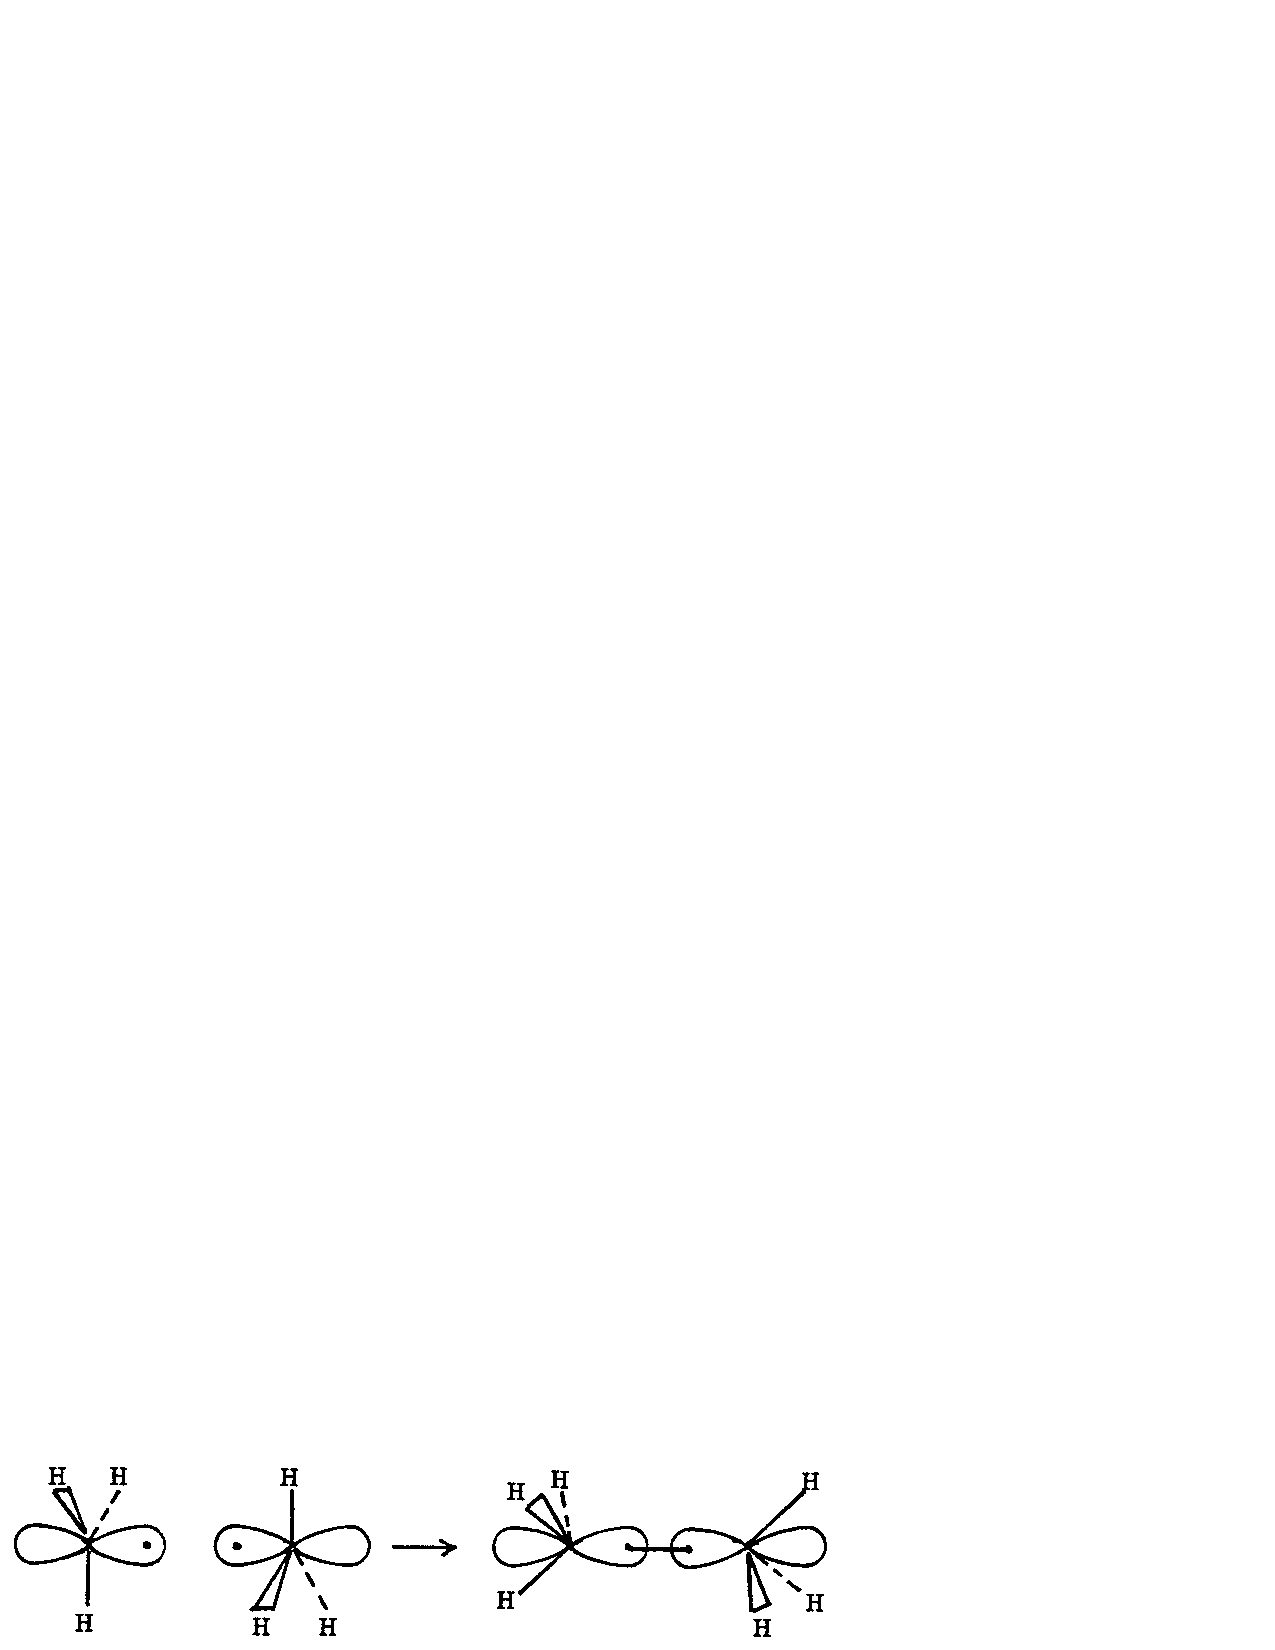
\includegraphics[scale=0.75]{fg7b}
\label{chap7-eqno2}
\end{equation}
Just as with methane, the CH bond orbitals must remain orthogonal to
the newly formed CC bond, Pauli principle, with the result that the
geometry at each C is roughly tetrahedral.  Of course, the CH and CC
bond orbitals are not equivalent and hence, the geometry is not quite
tetrahedral.  In fact, the HCC angle is 111.2$^{\circ}$ while the HCH
angle is 107.7$^{\circ}$.  There is not an accurate spectroscopic
value for C$_2$H$_6$.  These are based on trends in other alkanes.
This suggests that interaction of the CH bond with the CC bond is more
unfavorable than interaction of the CH bond with an adjacent CH bond.

Next we must consider the orientation of the CH bonds on one C 
relative to the CH bonds on the adjacent one.  The dominant effect 
arises from the Pauli principle, namely that the CH bonds on 
different carbons must get orthogonal. In order to keep this 
effect at a minimum, the geometry with lowest overlap between 
CH bonds on different carbon atoms is favored.  The extreme 
cases are staggered and eclipsed with staggered favored.
\begin{equation}
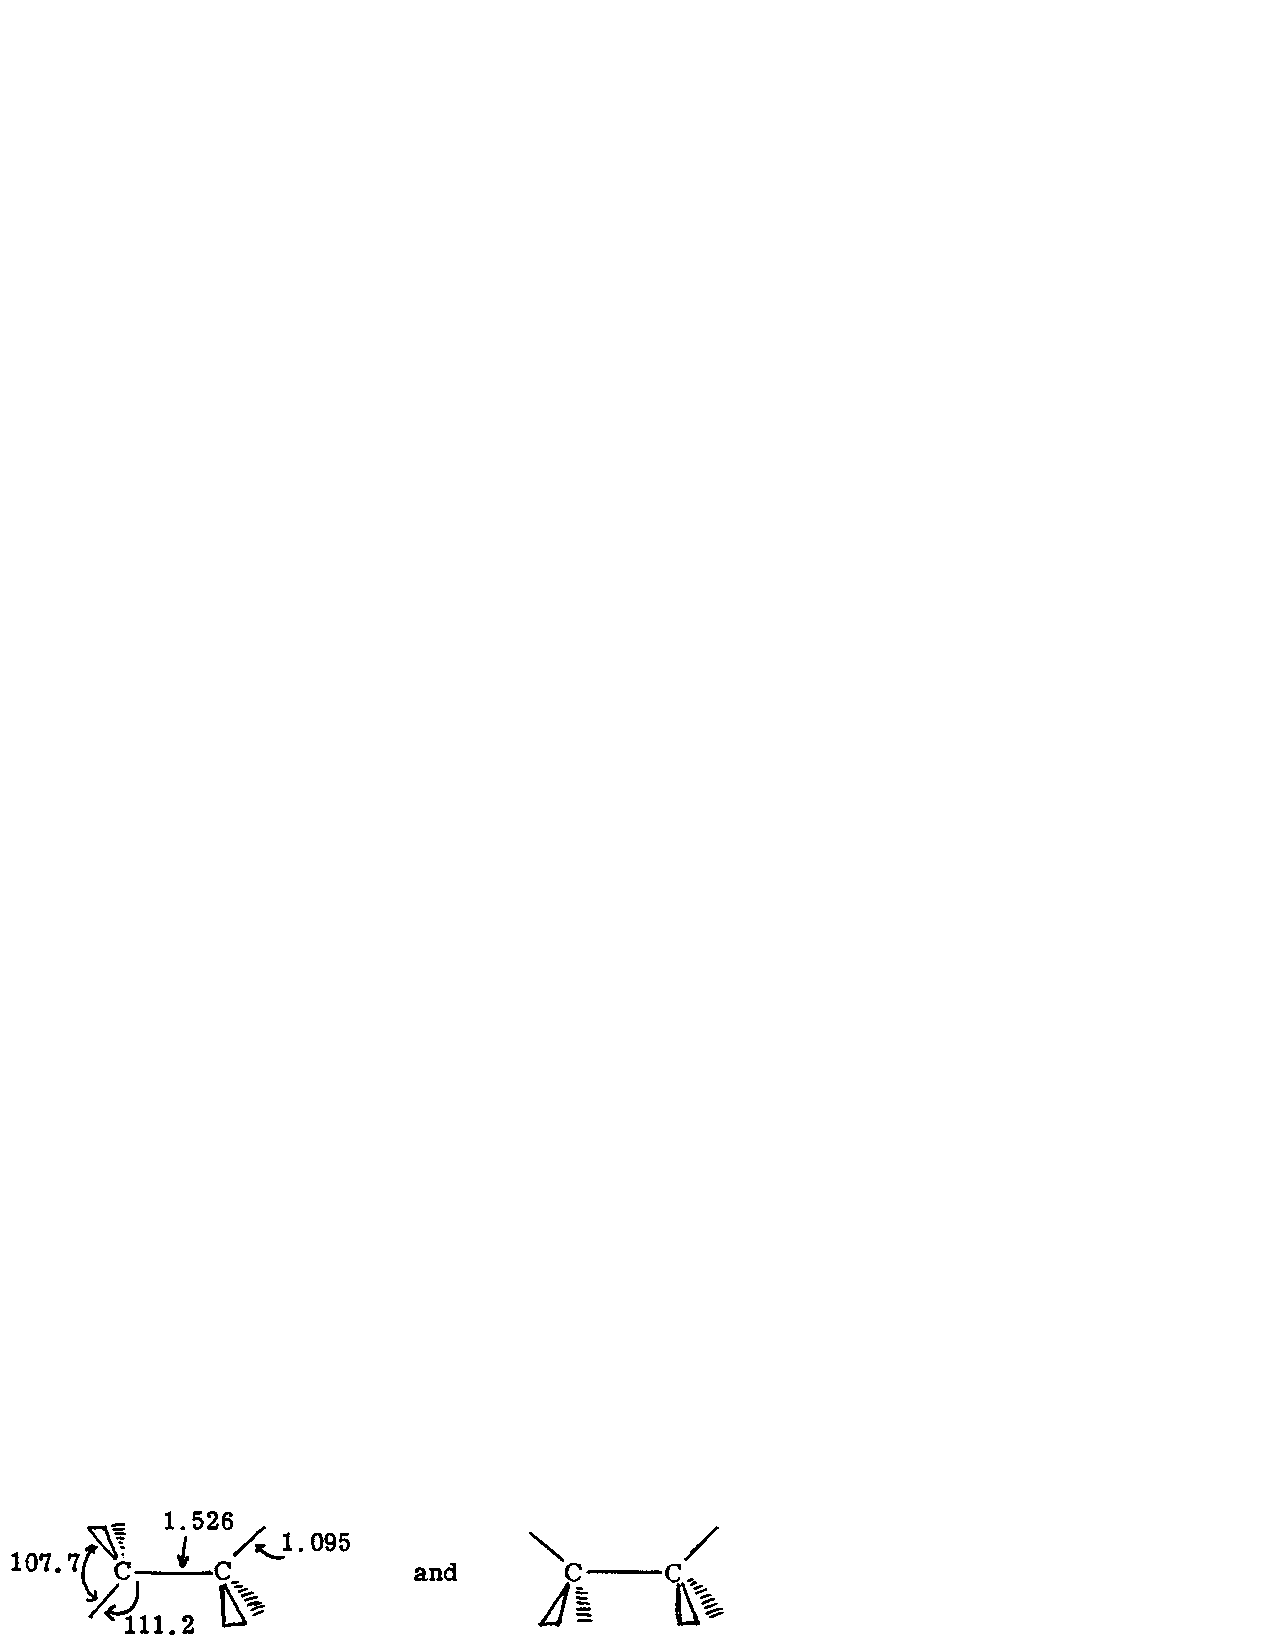
\includegraphics{fg7c}
\label{chap7-eqno3}
\end{equation}
The staggered (left) has the least overlap, and the eclipsed (right)
has the most overlap.

The potential curve, for rotation of one group relative to the other,
has the form in Figure \ref{chap7-fig1}, with a well depth of 3 kcal.
The orbitals, from self-consistent generalized valence bond
calculations \cite{chap7-ref1} on ethane, are shown in Figure
\ref{chap7-fig2} and compared to those of methane in Figure
\ref{chap7-fig3}.


\begin{figure}
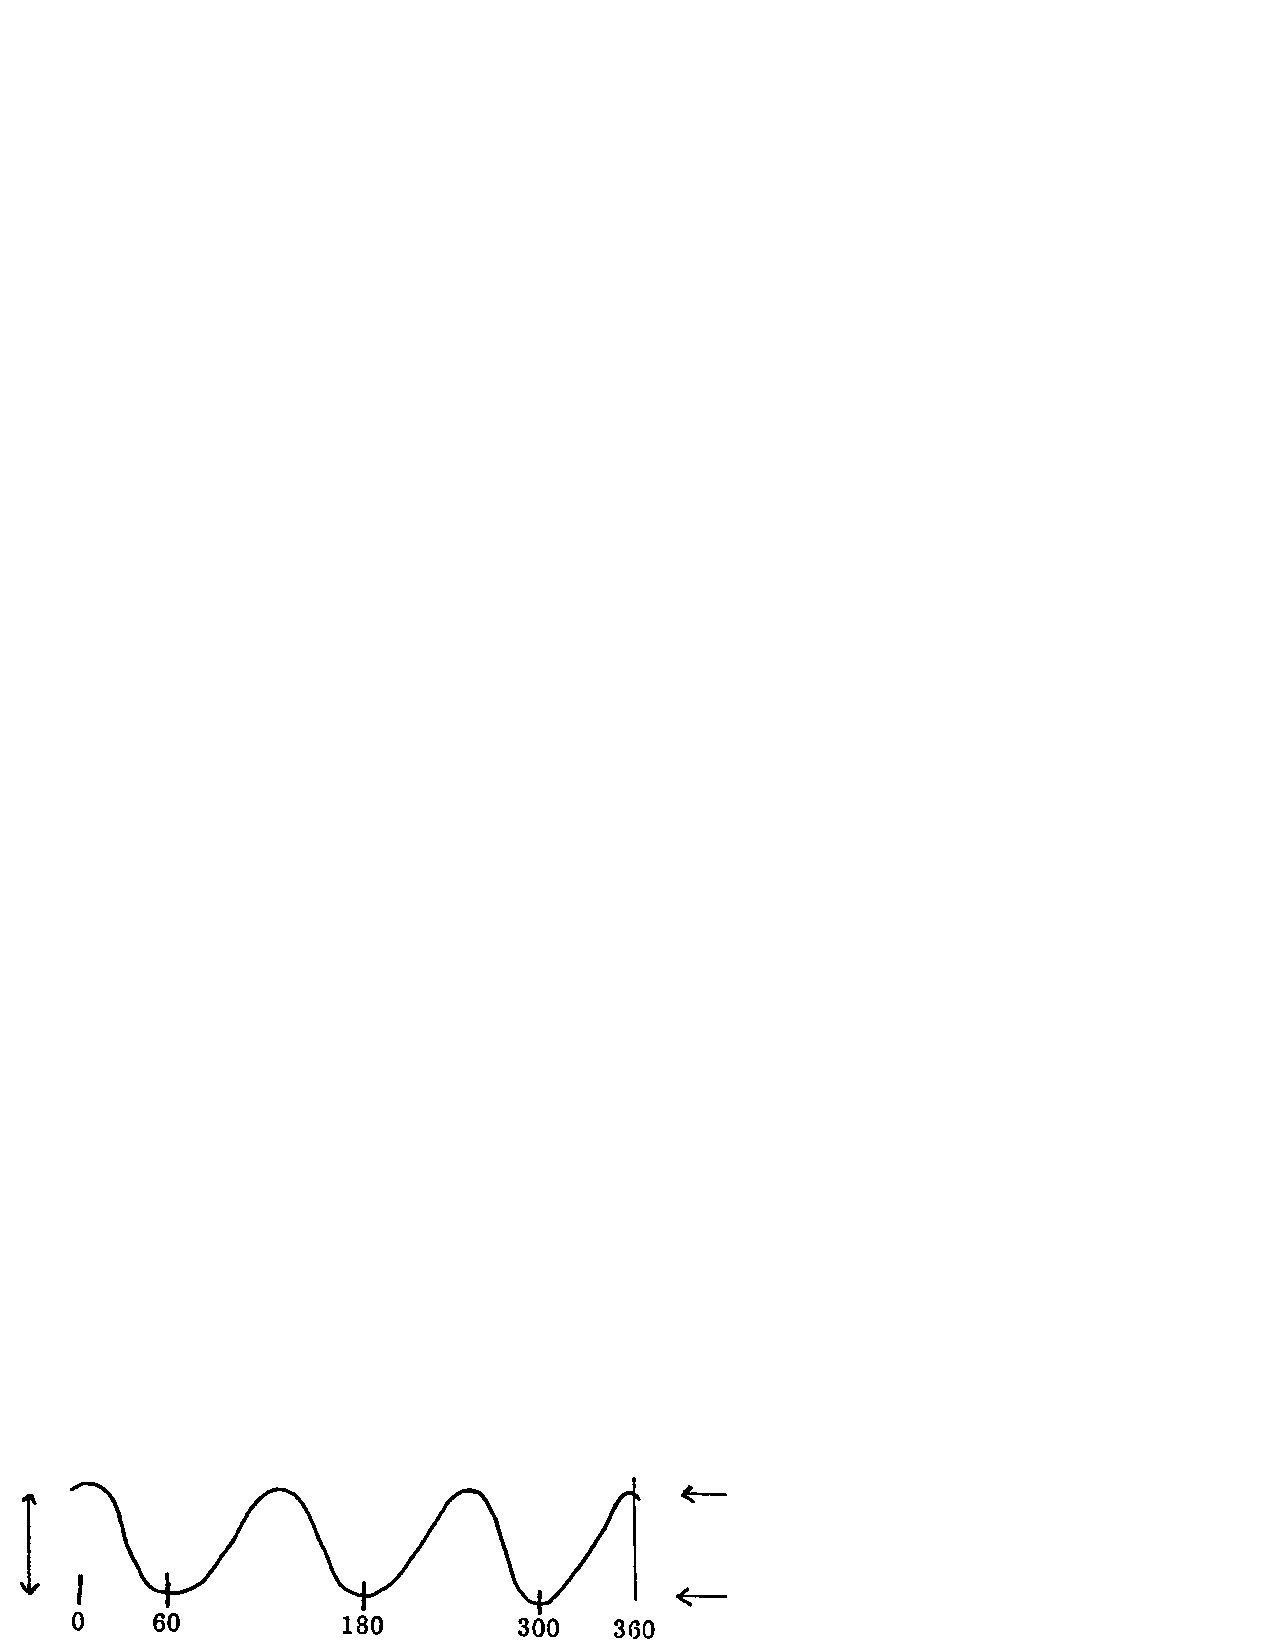
\includegraphics[scale=0.75]{fg7-1}
\caption{}
\label{chap7-fig1}
\end{figure}

\begin{figure}
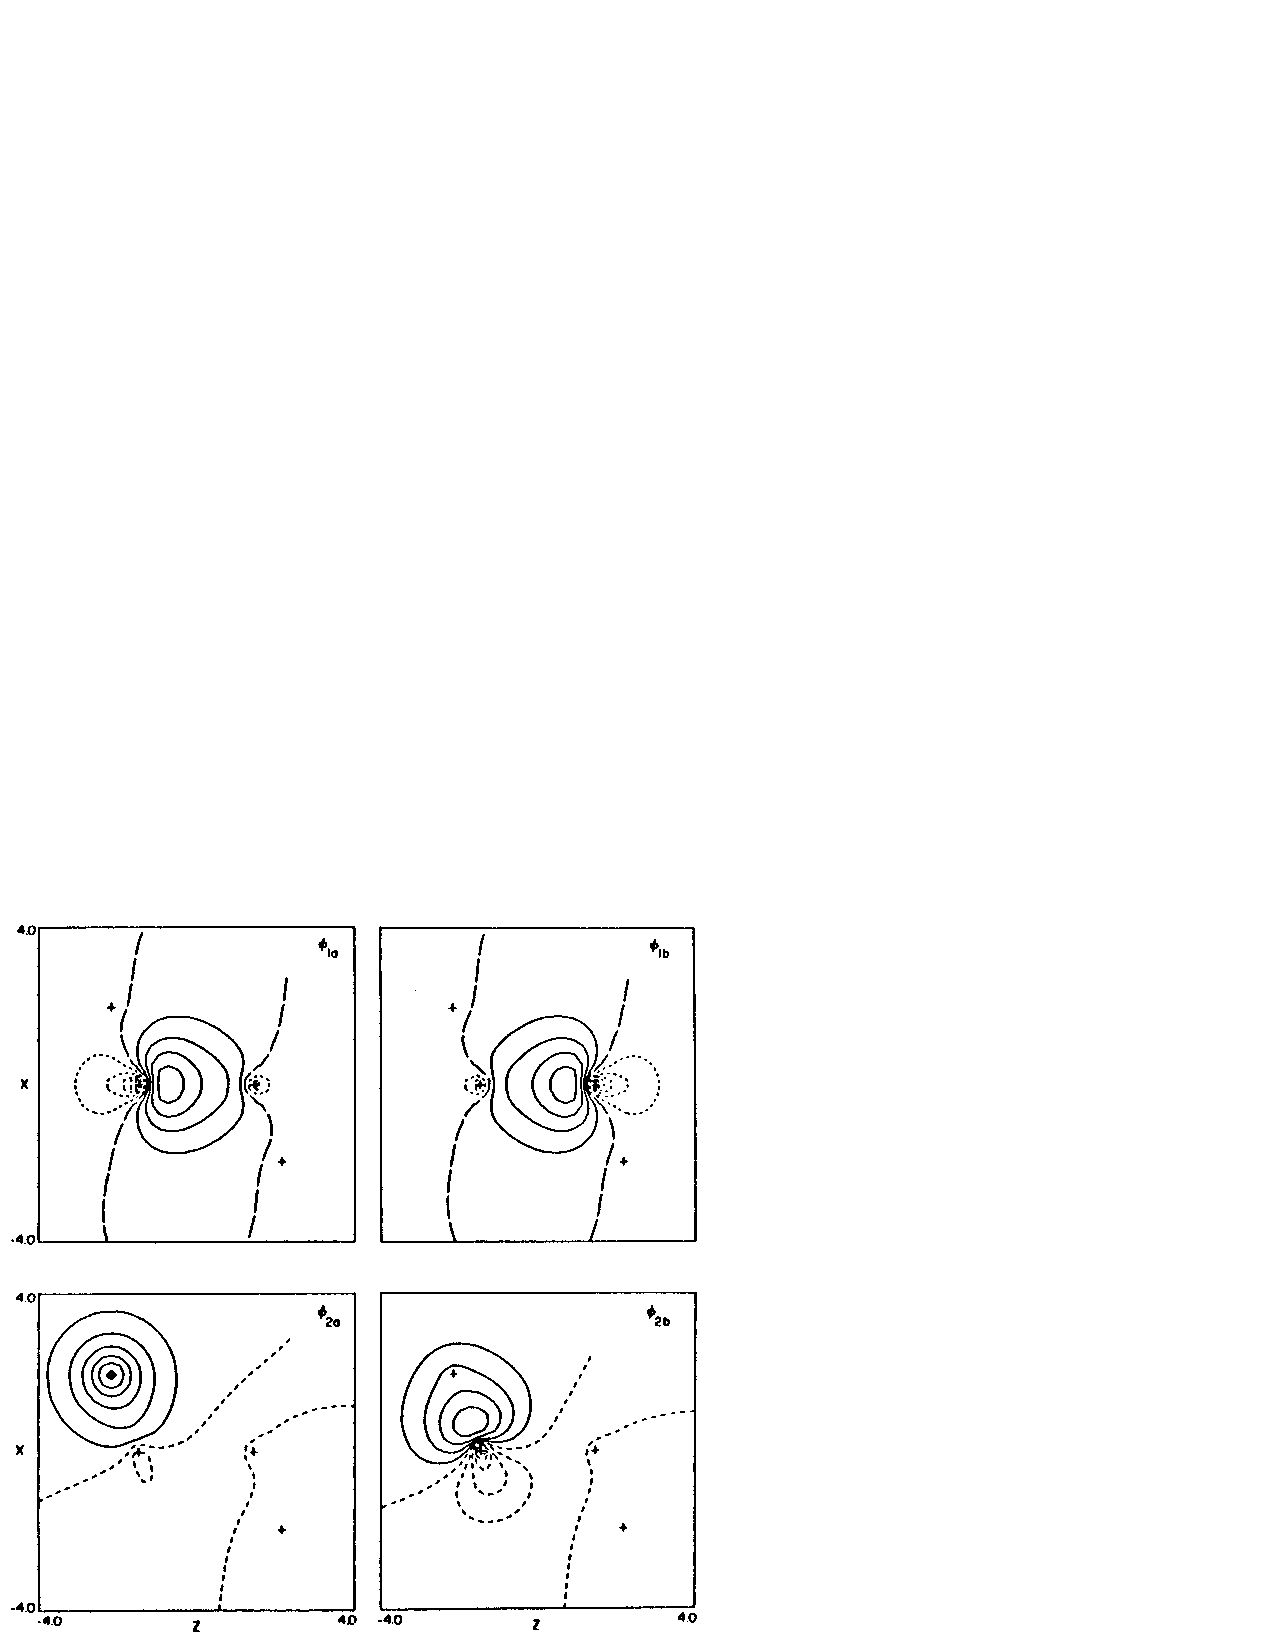
\includegraphics[scale=0.75]{fg7-2}
\caption{Bonding orbitals in staggered ethane.}
\label{chap7-fig2}
\end{figure}

\begin{figure}
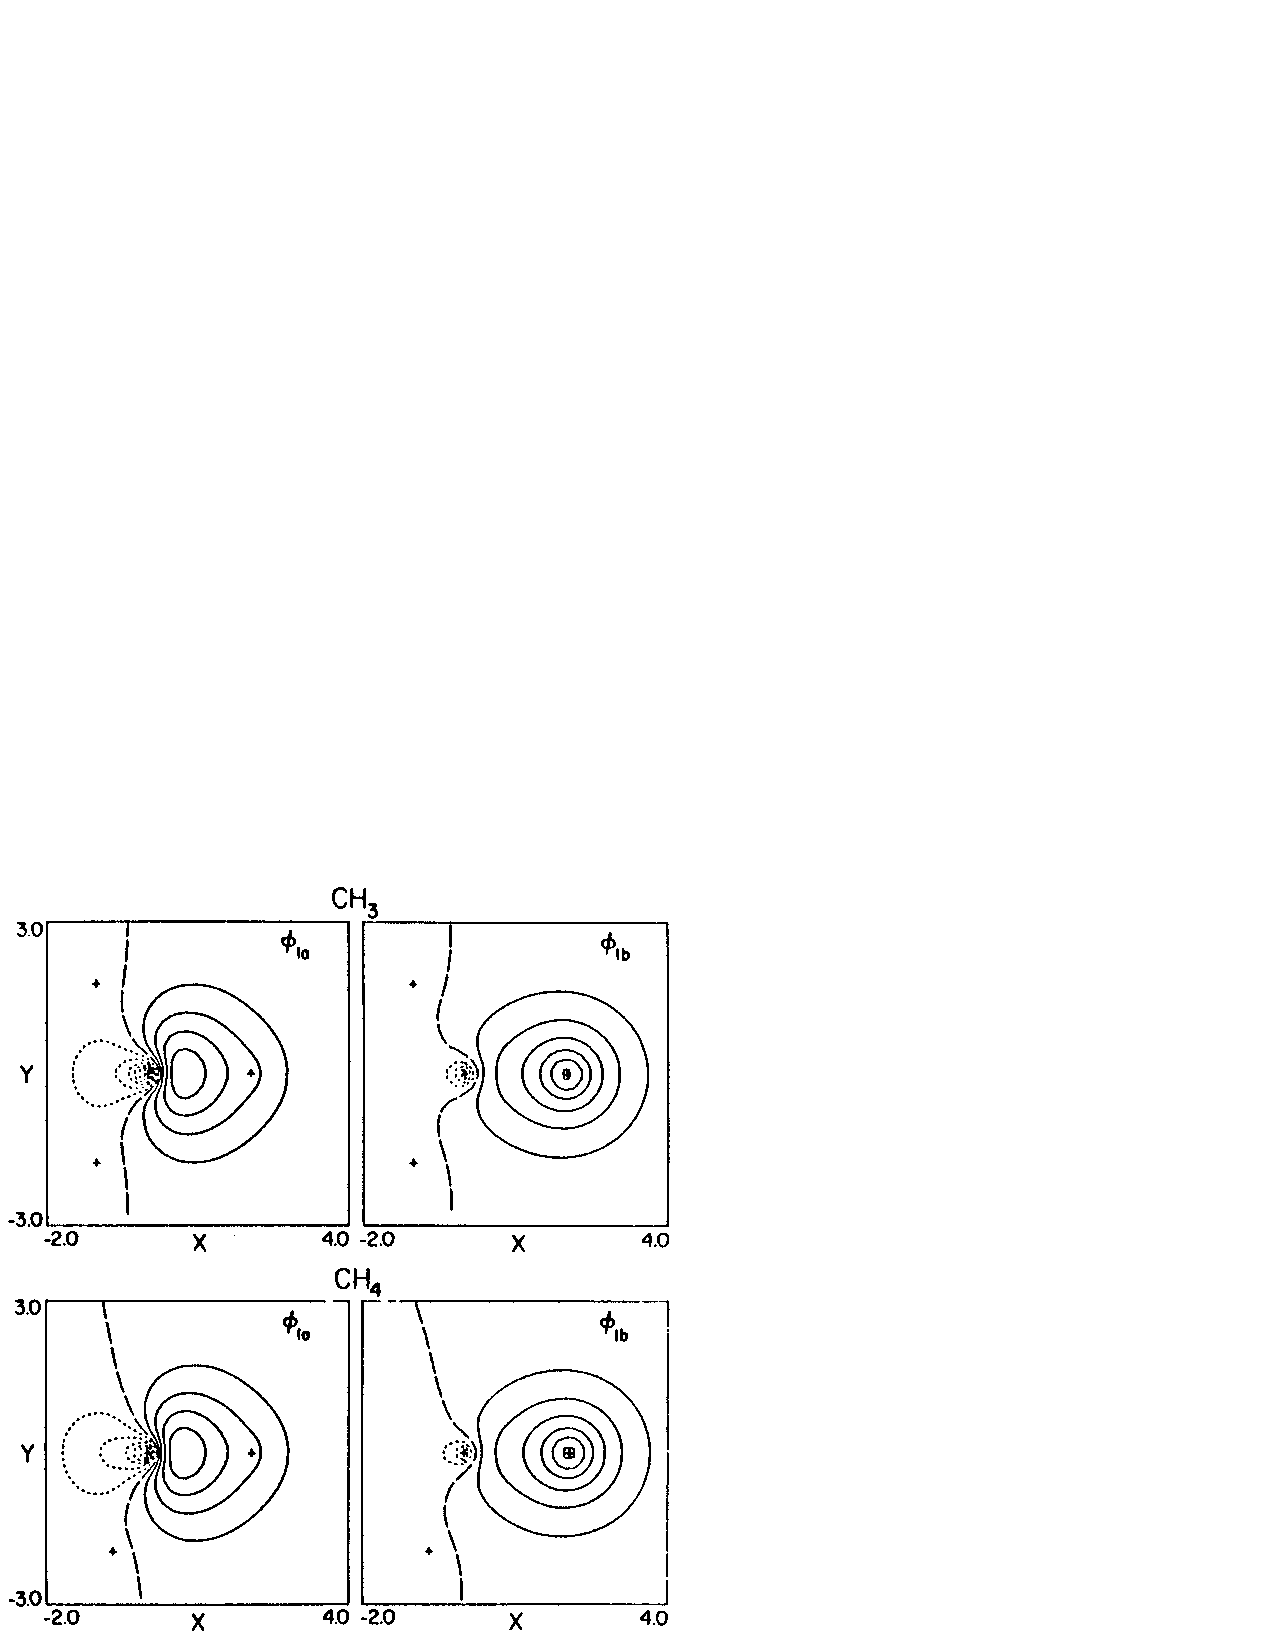
\includegraphics[scale=0.75]{fg7-3}
\caption{Bonding orbitals in methane.}
\label{chap7-fig3}
\end{figure}


\subsection{Propane}

Now consider replacing one of the CH bonds, in ethane, with a bond 
to a methyl group to yield propane
\begin{equation}
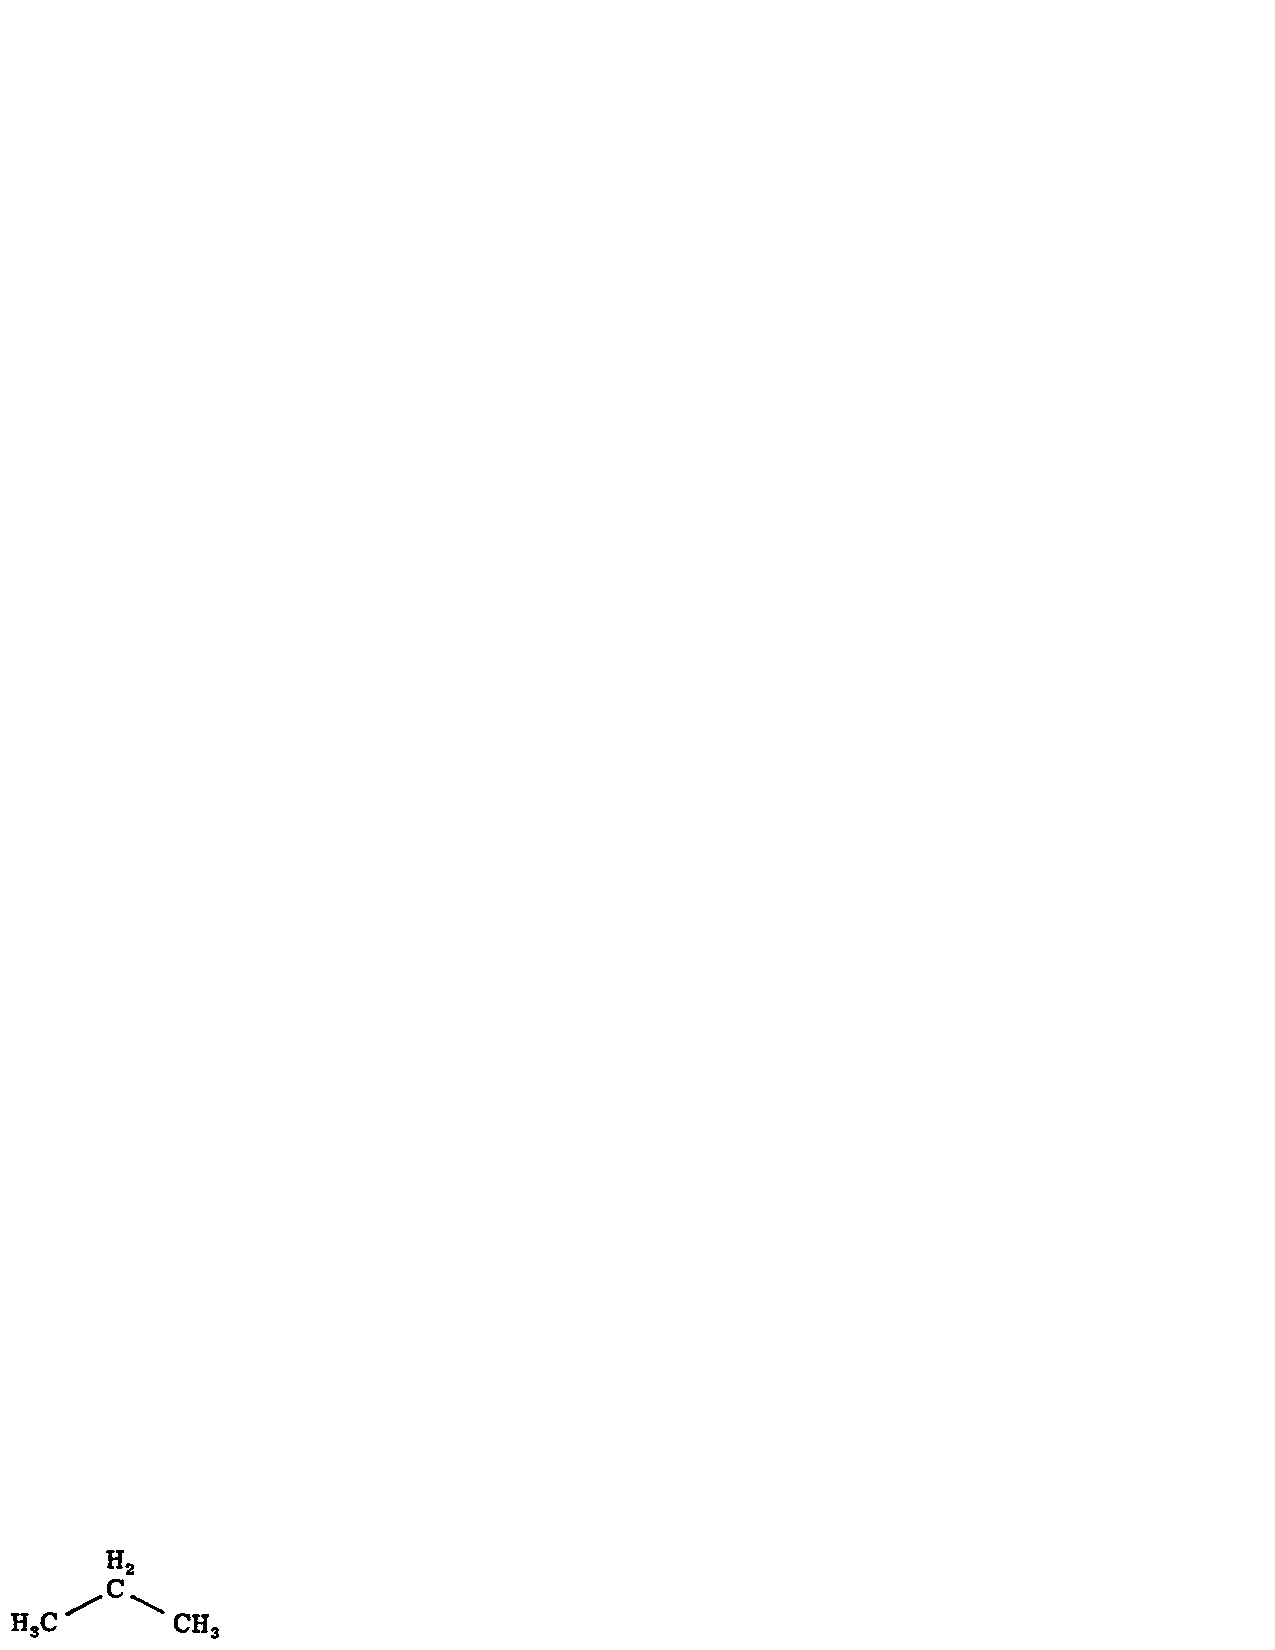
\includegraphics{fg7-1a}
\label{chap7-eqno4}
\end{equation}
Keeping both methyl groups staggered leads to the geometry
\begin{equation}
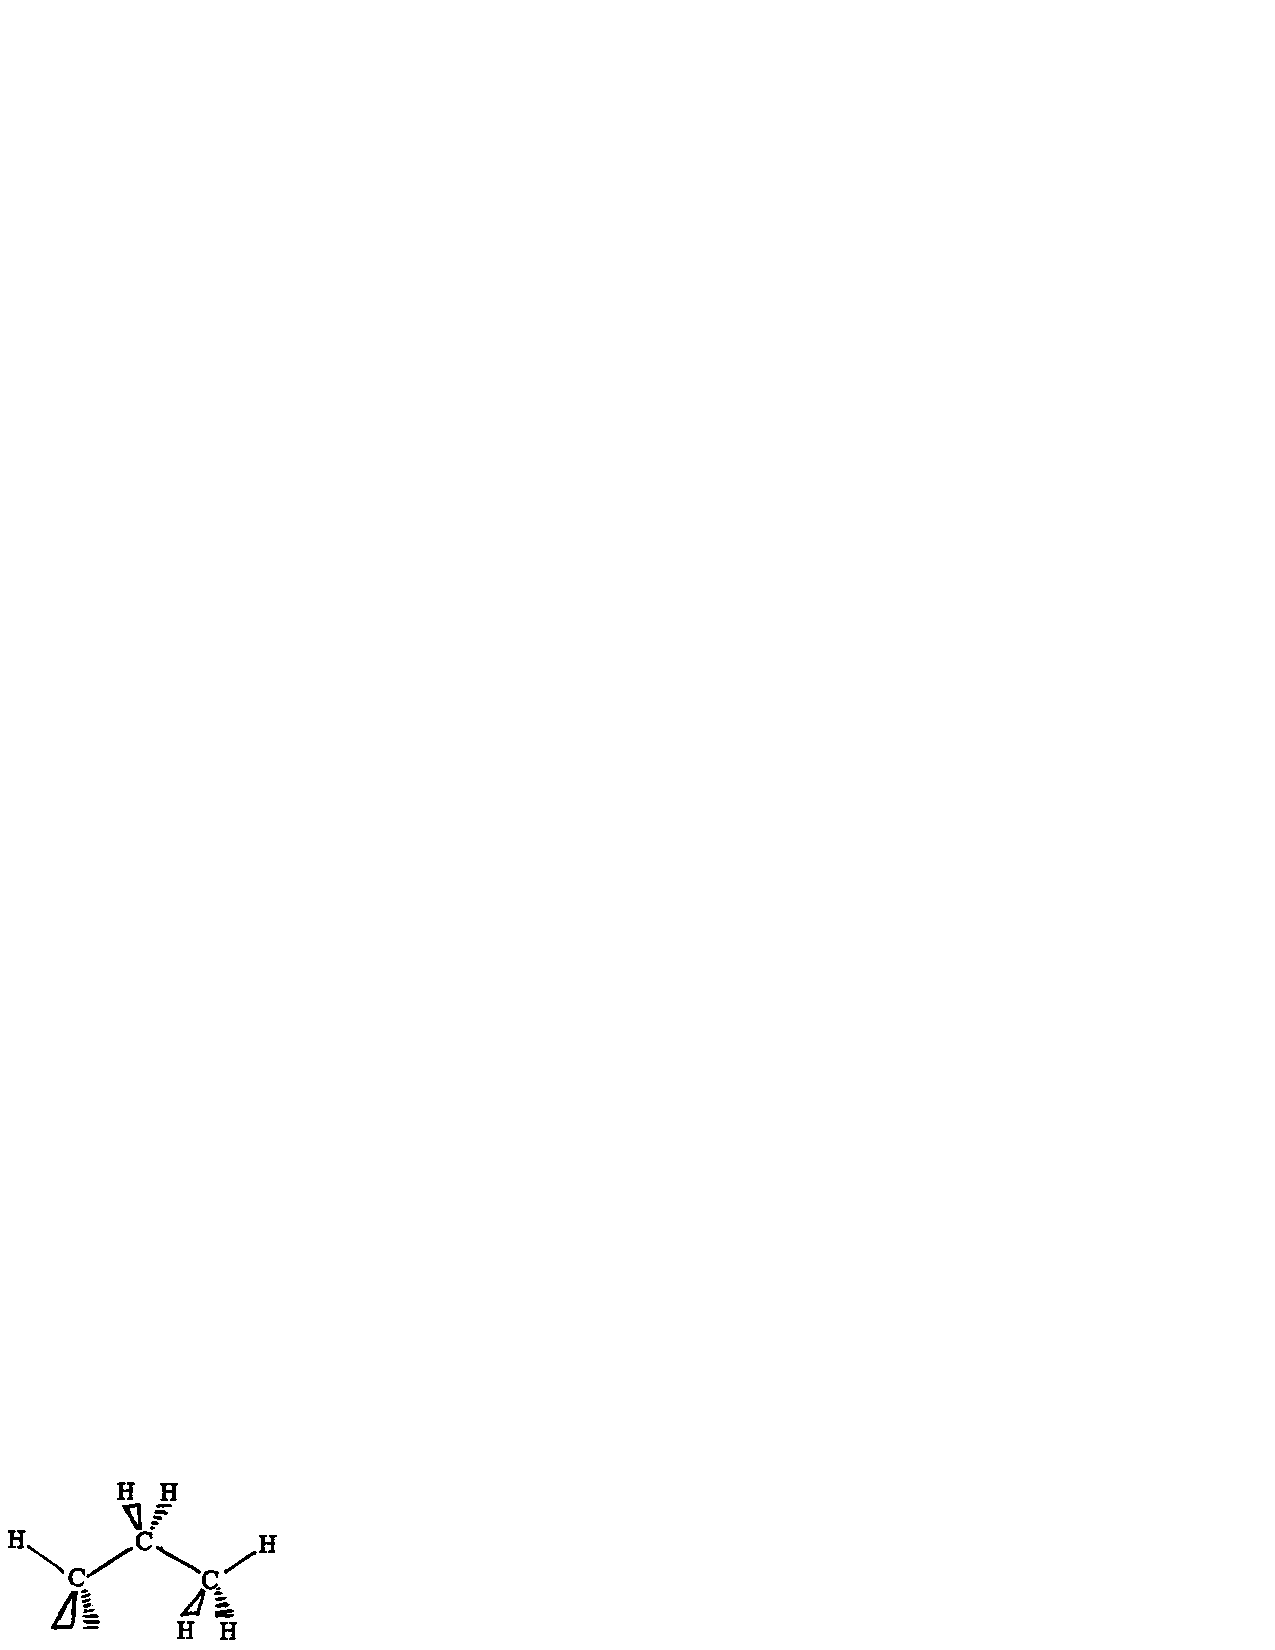
\includegraphics{fg7-3a}
\label{chap7-eqno5}
\end{equation}
Now consider the details of the geometry
\begin{equation}
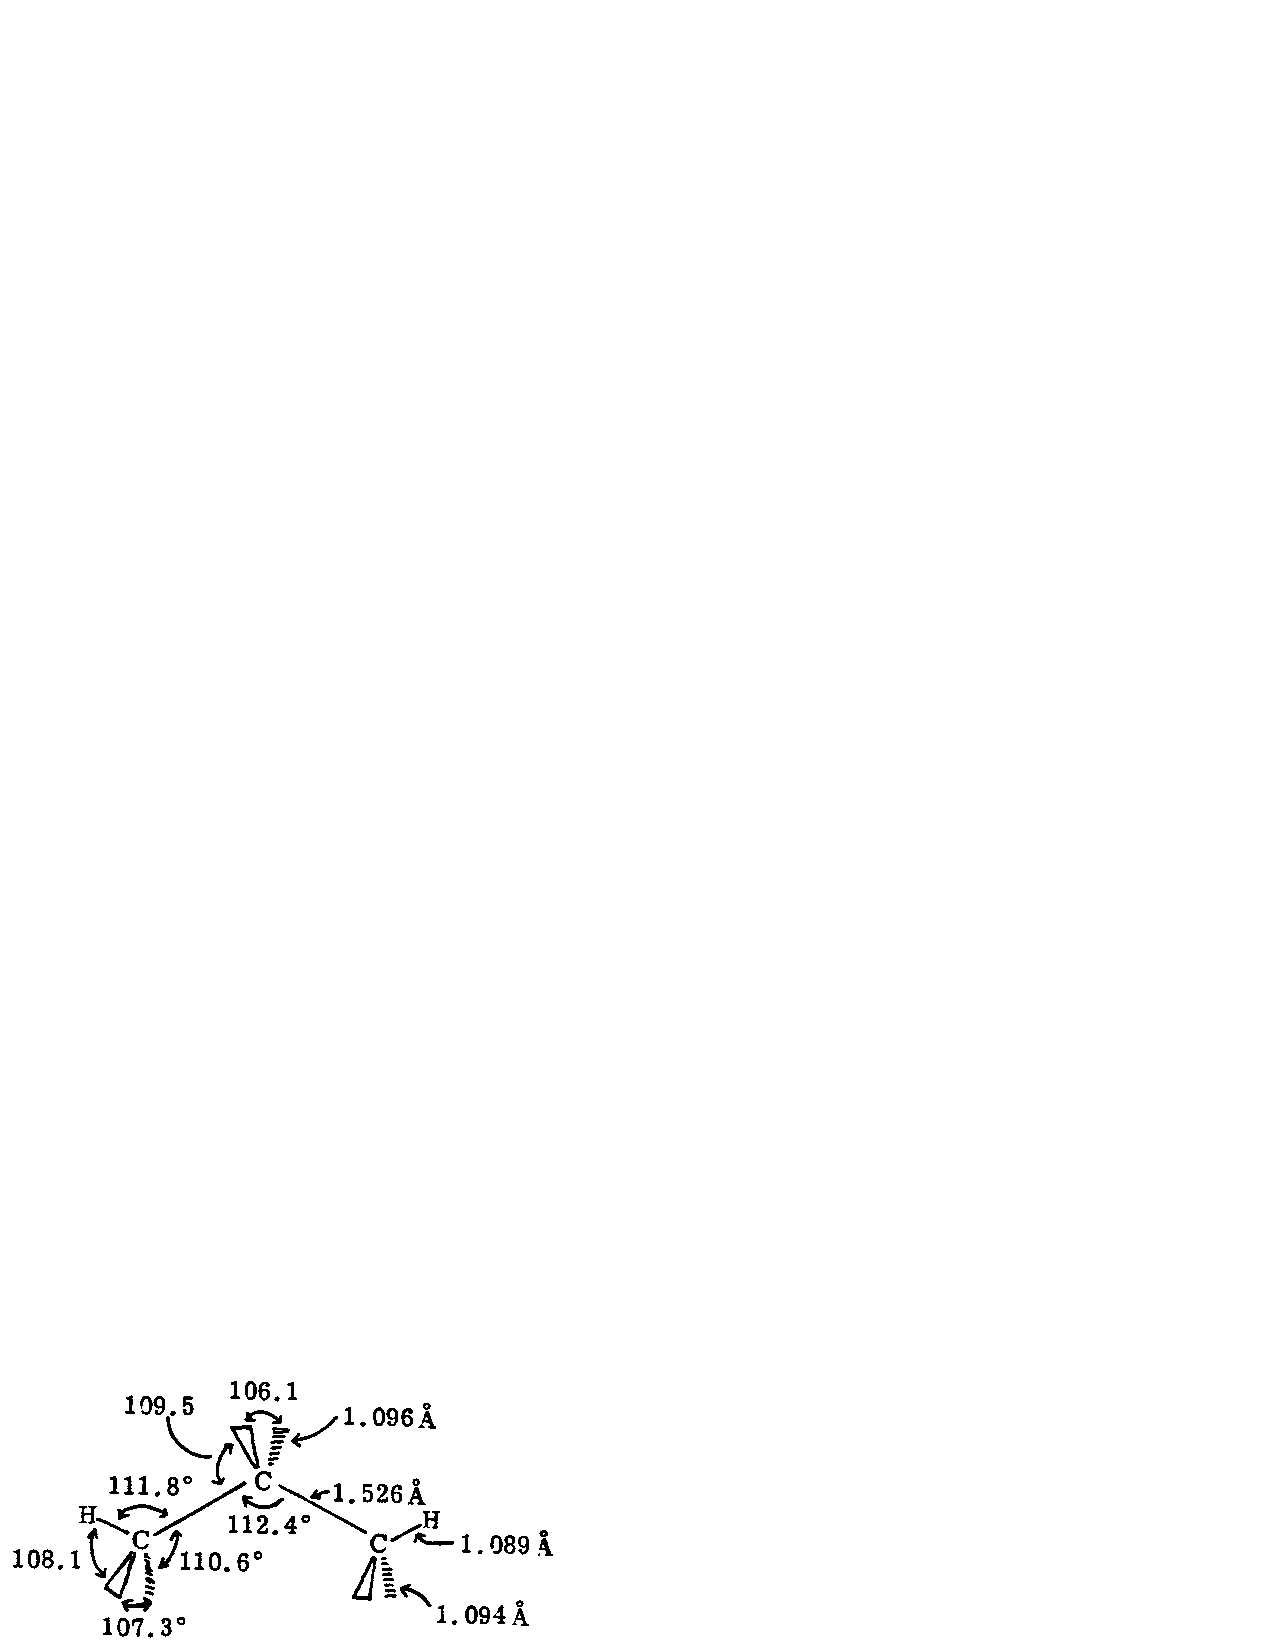
\includegraphics{fg7-3b}
\label{chap7-eqno6}
\end{equation}
The CCC angle is 112.4$^{\circ}$, indicating that repulsive interactions 
between the C-C bonds dominate, between the two methyl groups. The 
angles between a CH bond of the center carbon and a CC bond is 
109.5$^{\circ}$, there are four such cases, just the tetrahedral value. The 
angle between the two CH bonds of the centered carbon is 
106.1$^{\circ}$.  As for C$_2$H$_6$, this indicates that CH-CC 
interactions are stronger than CH-CH interactions.

\subsection{Trends in Geometries}

Comparing the geometries of saturated hydrocarbons that have 
been studied by microwave spectroscopy, CH$_4$, C$_3$H$_8$, and 
iso-C$_4$H$_{10}$, leads to the following systematics:
\begin{enumerate}
\item The CH bond length is 1.095 $\pm$ 0.001 \AA.  Exceptions to 
this are a CH bond trans to a CC bond, it is 1.089 \AA, and 
a CH bond trans to three CH bonds, is 1.108 \AA.

\item The CC bond length is 1.526 $\pm$ 0.001 \AA.

\item CCC angles are 
\begin{equation}
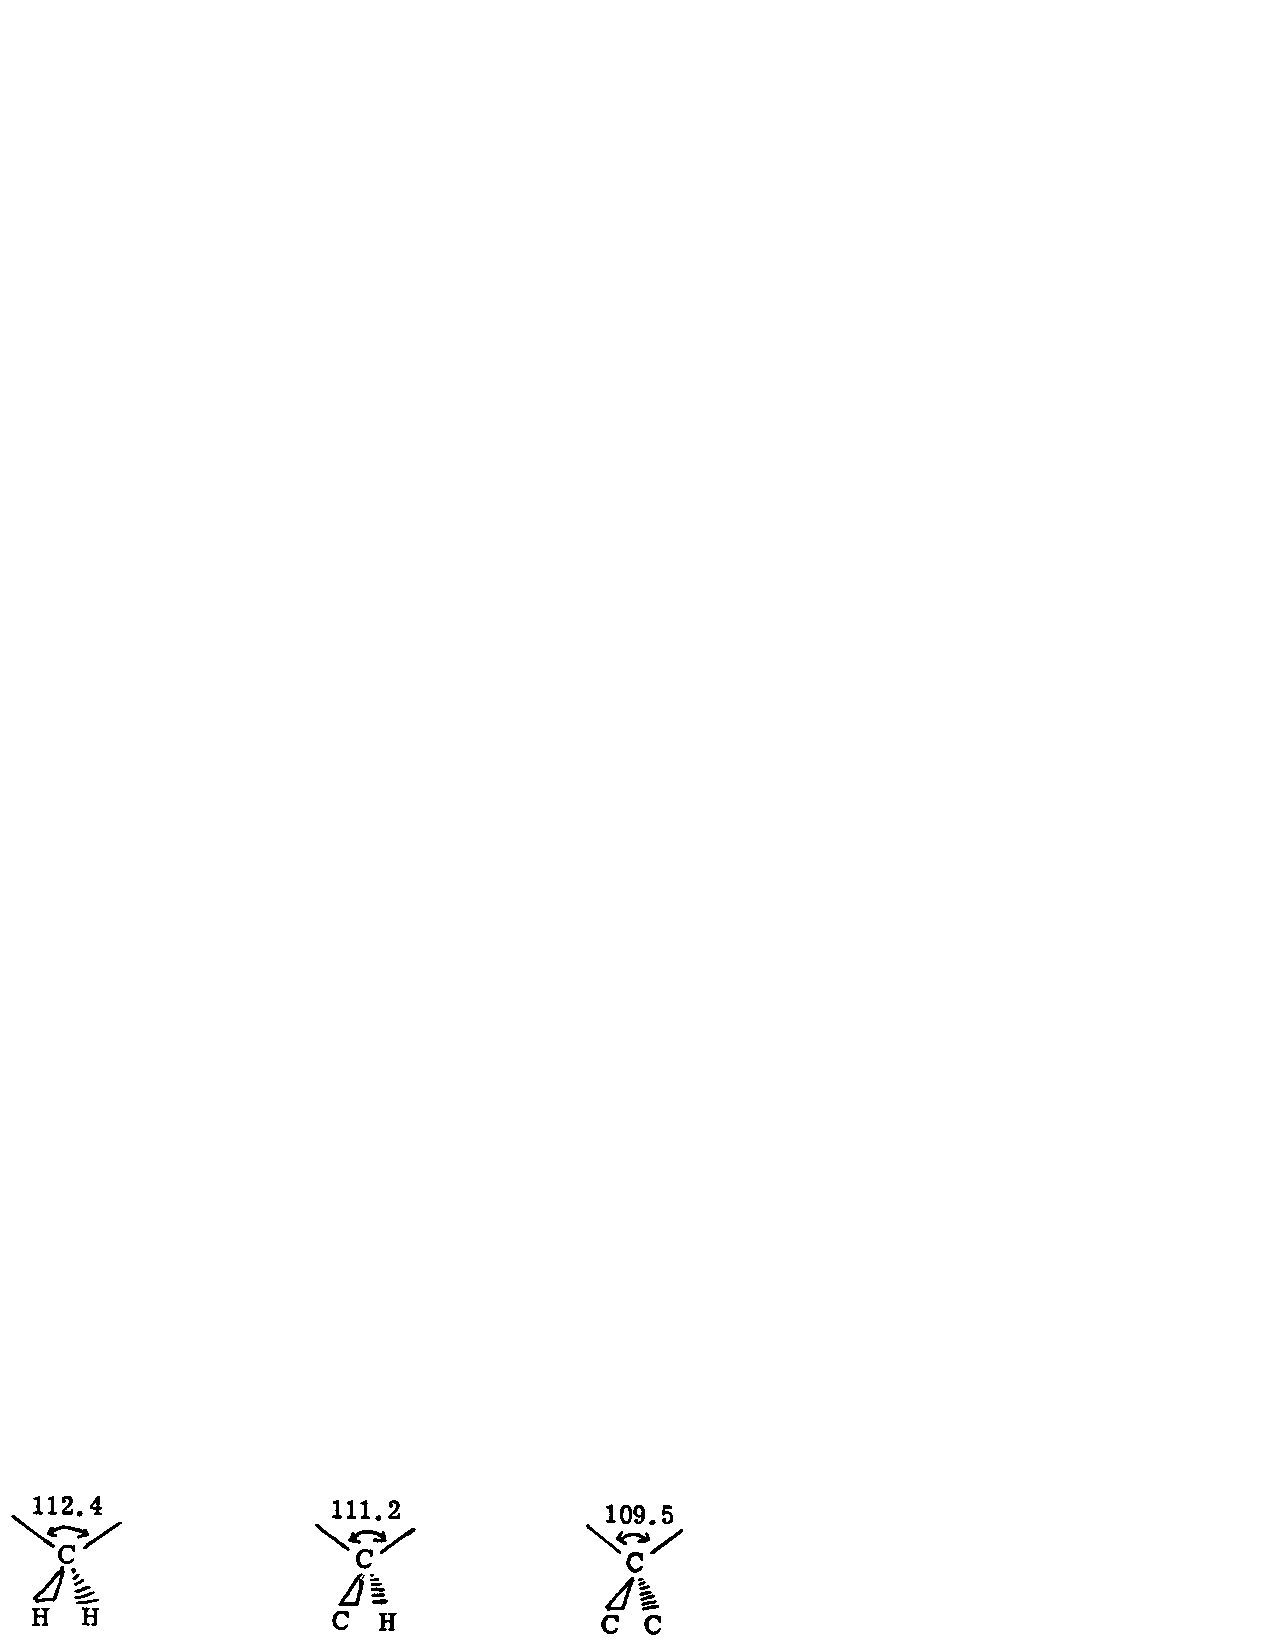
\includegraphics{fg7-3c}
\label{chap7-eqno7}
\end{equation}

\item HCH angles are as follows:
\begin{equation}
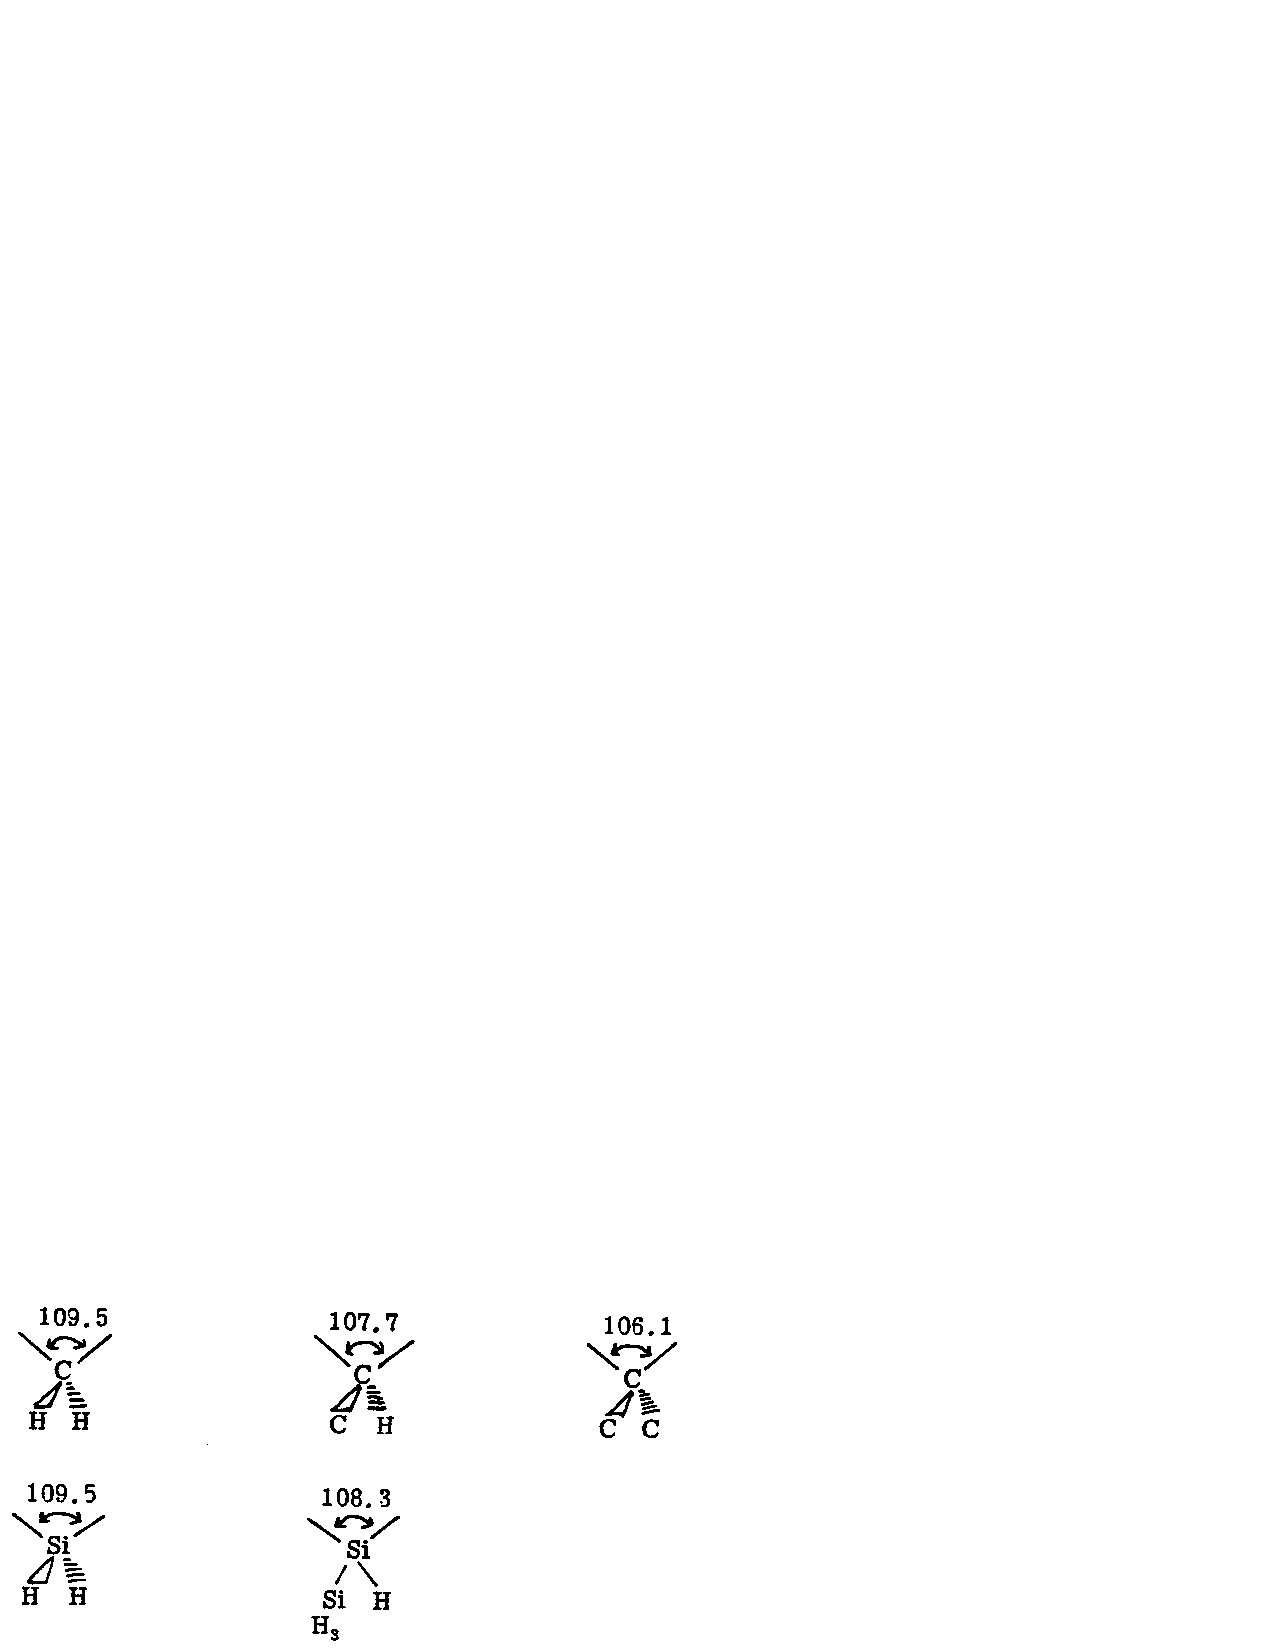
\includegraphics{fg7-3d}
\label{chap7-eqno8}
\end{equation}
\end{enumerate}

\subsection{Diamond}

Starting with ethane and replacing all CH bonds with Me groups, leads
to
\begin{equation}
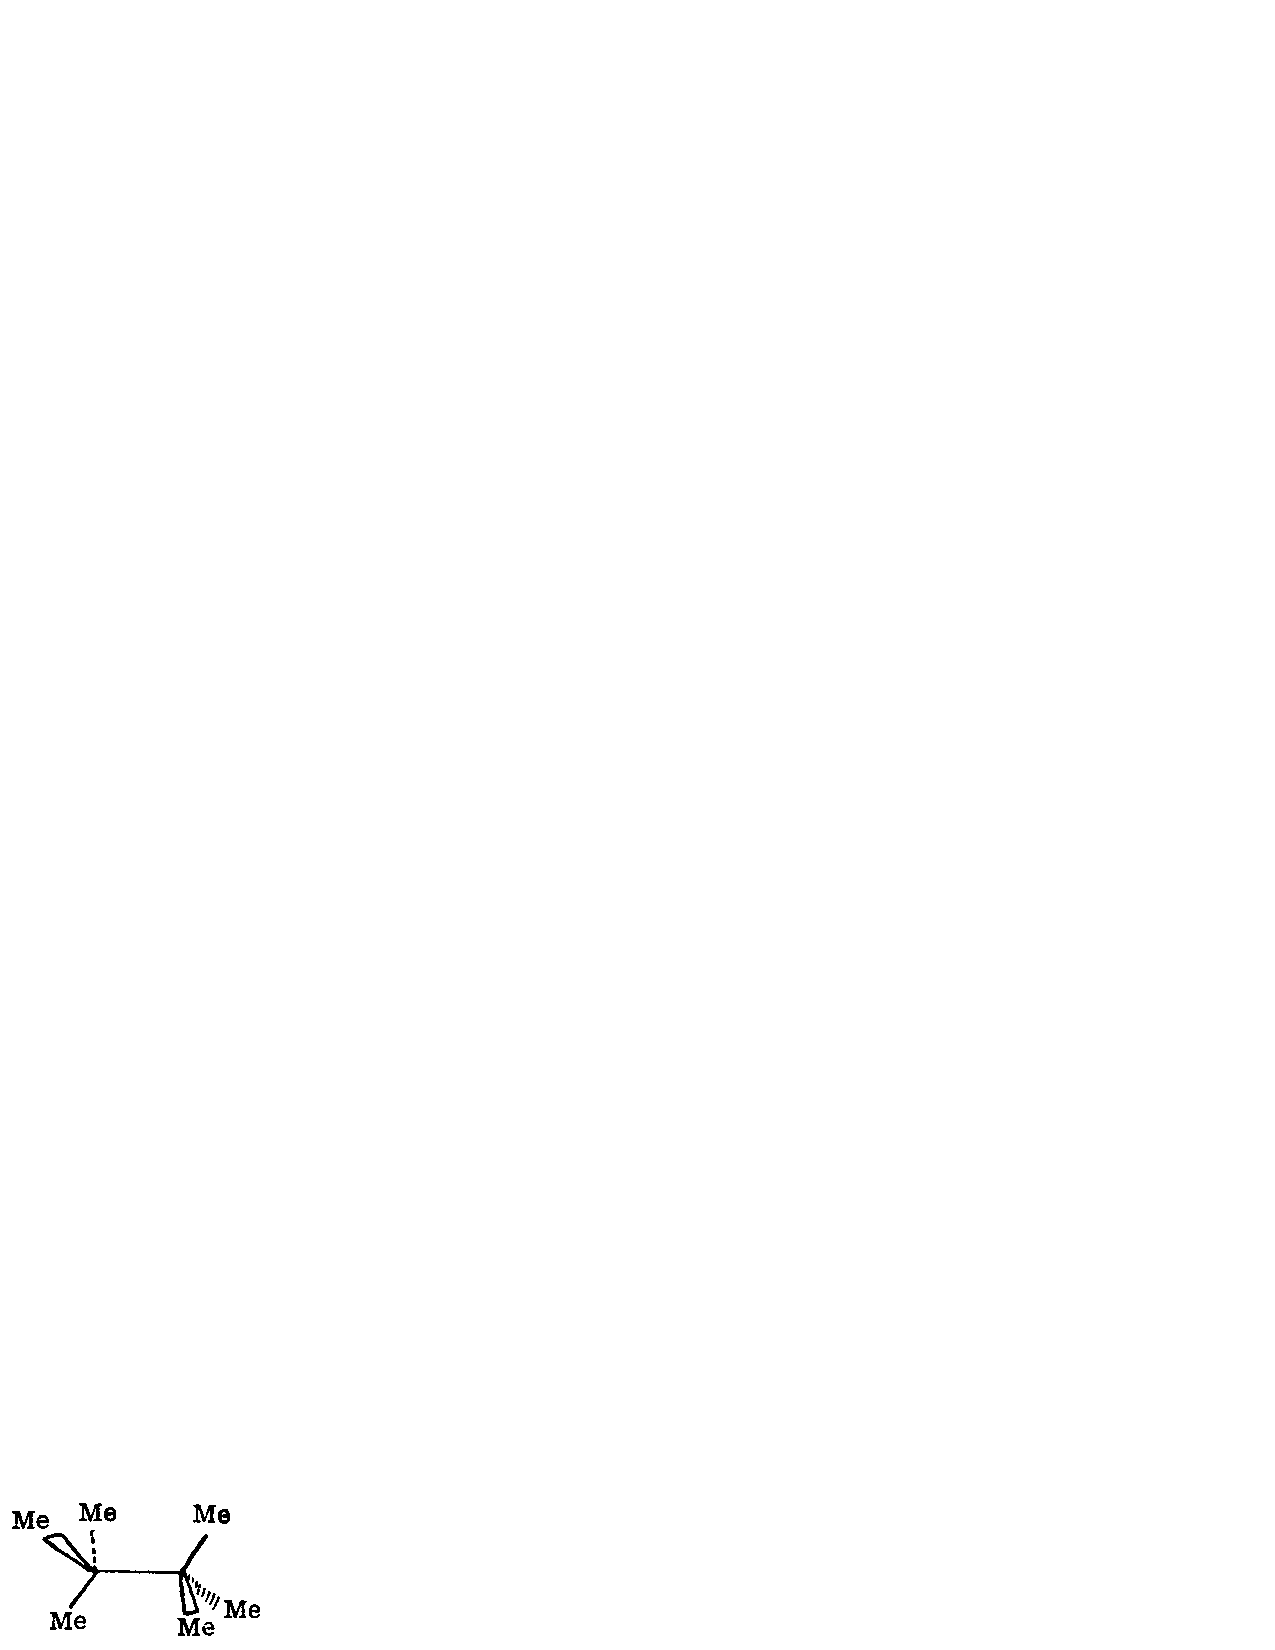
\includegraphics{fg7-3e}
\label{chap7-eqno9}
\end{equation}
with a staggered geometry.  Continuing to replace CH groups with Me 
groups \emph{ad infinitum} leads to diamond with all carbon atoms bonded 
tetrahedrically to other carbon atoms, and all bonds staggered with 
respect to those of adjacent carbons.  A side view is
\begin{equation}
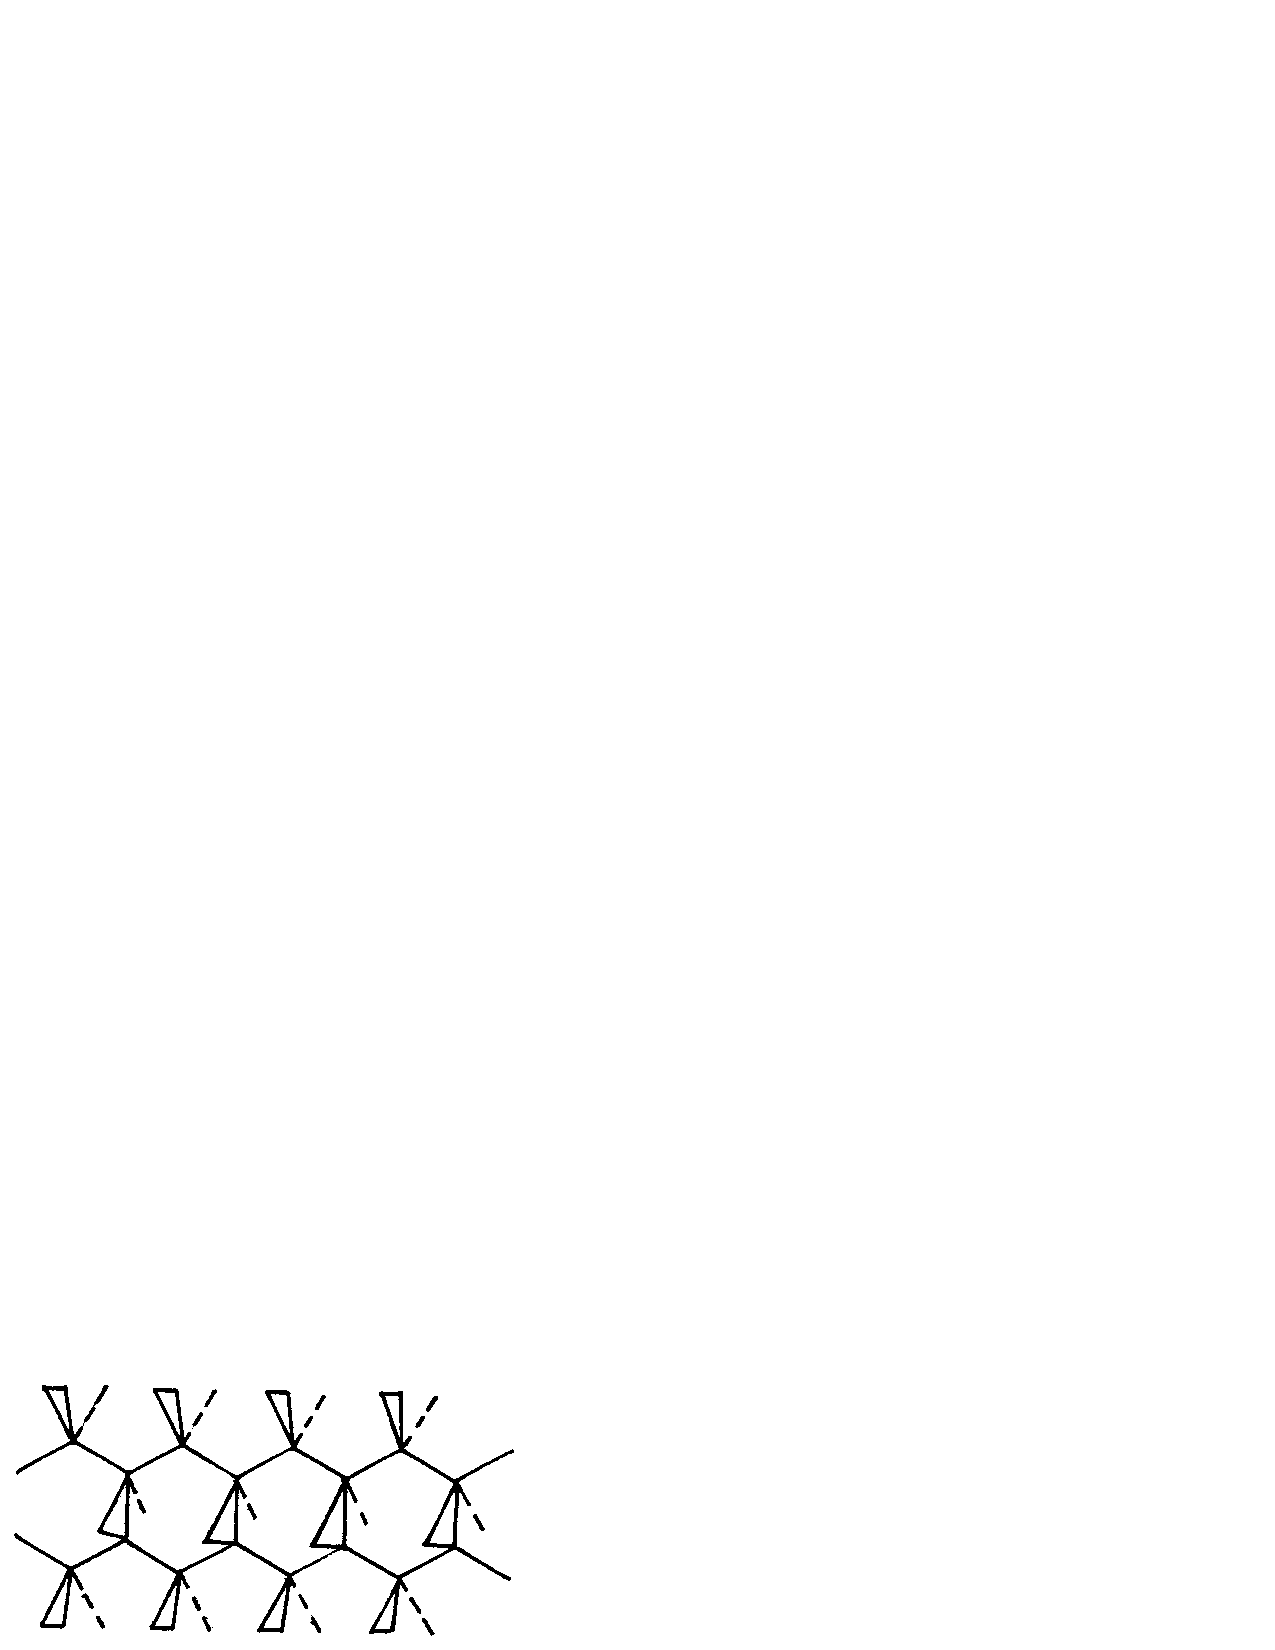
\includegraphics{fg7-3f}
\label{chap7-eqno10}
\end{equation}
Some aspects to notice in this structure are: 
\begin{enumerate}
\item staggered infinite chains
\begin{equation}
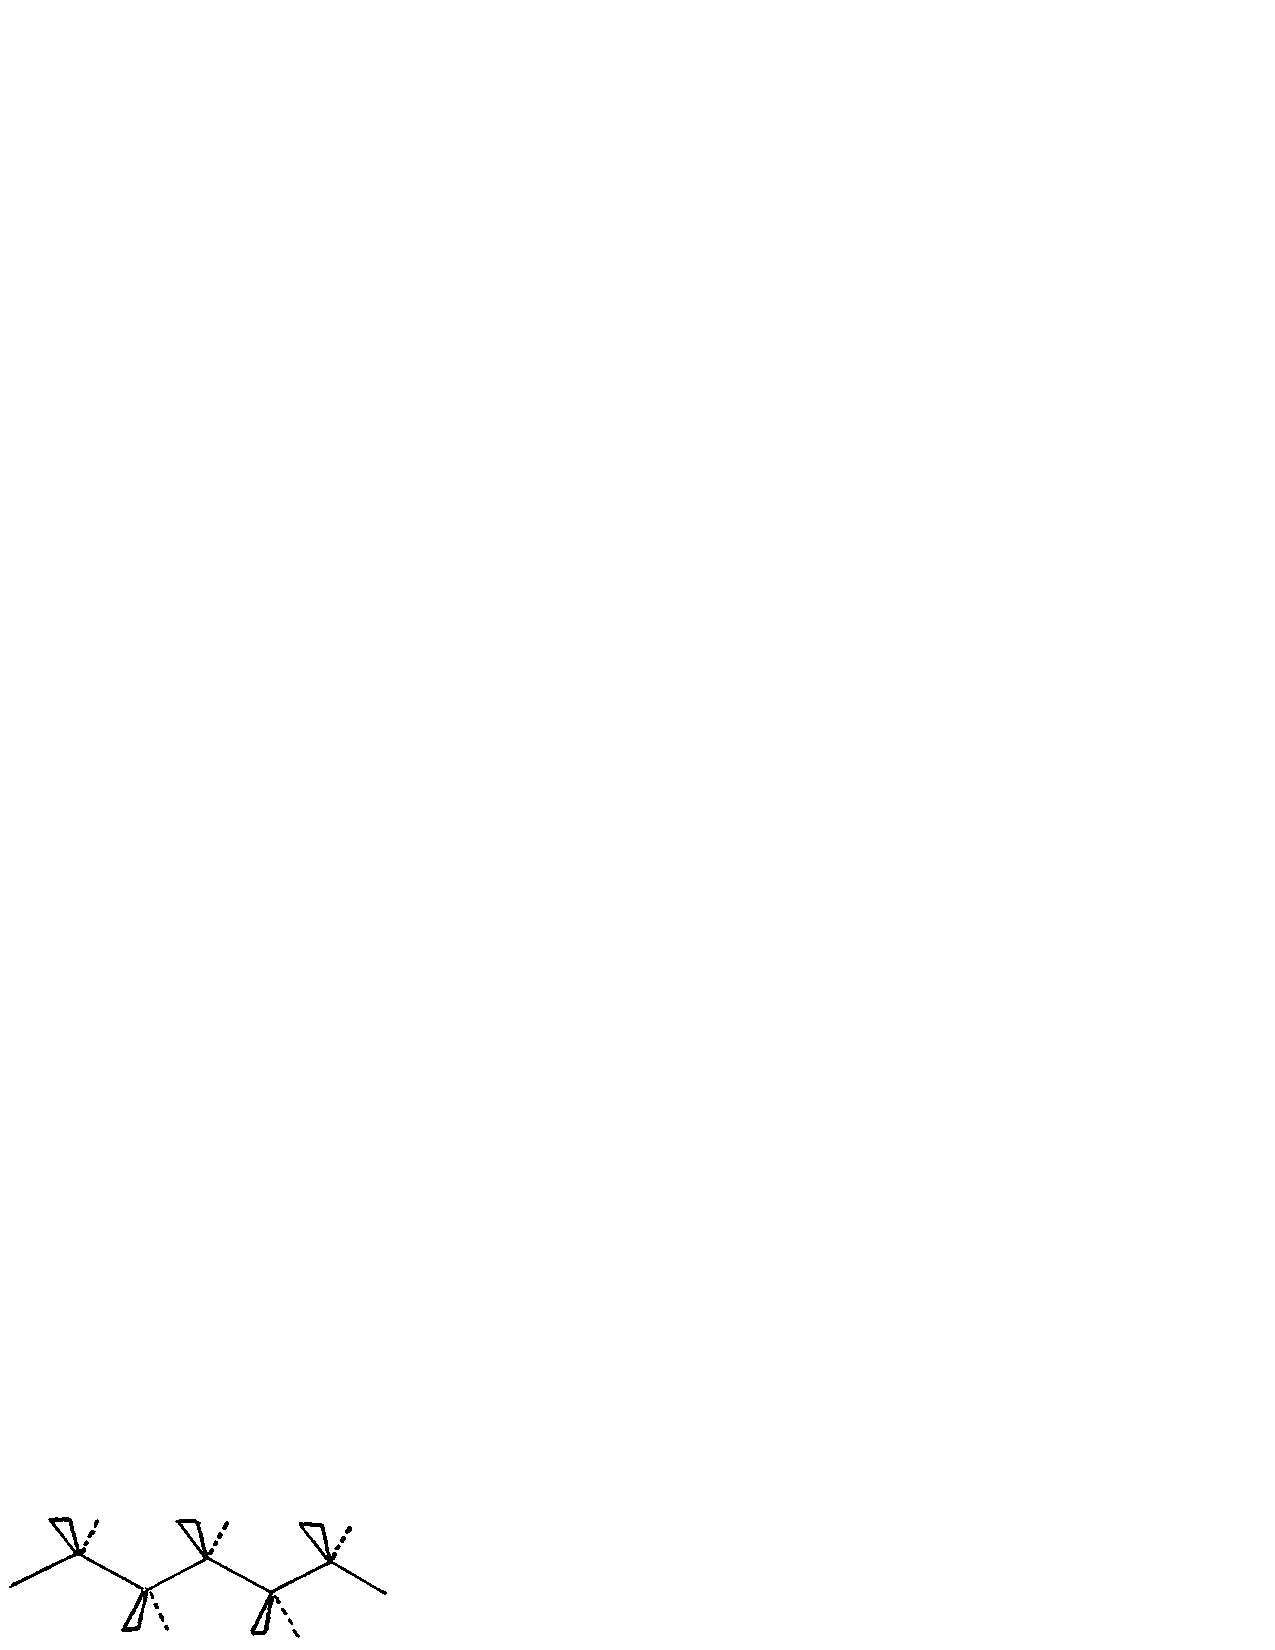
\includegraphics{fg7-3g}
\label{chap7-eqno11}
\end{equation}

\item six-membered rings
\begin{equation}
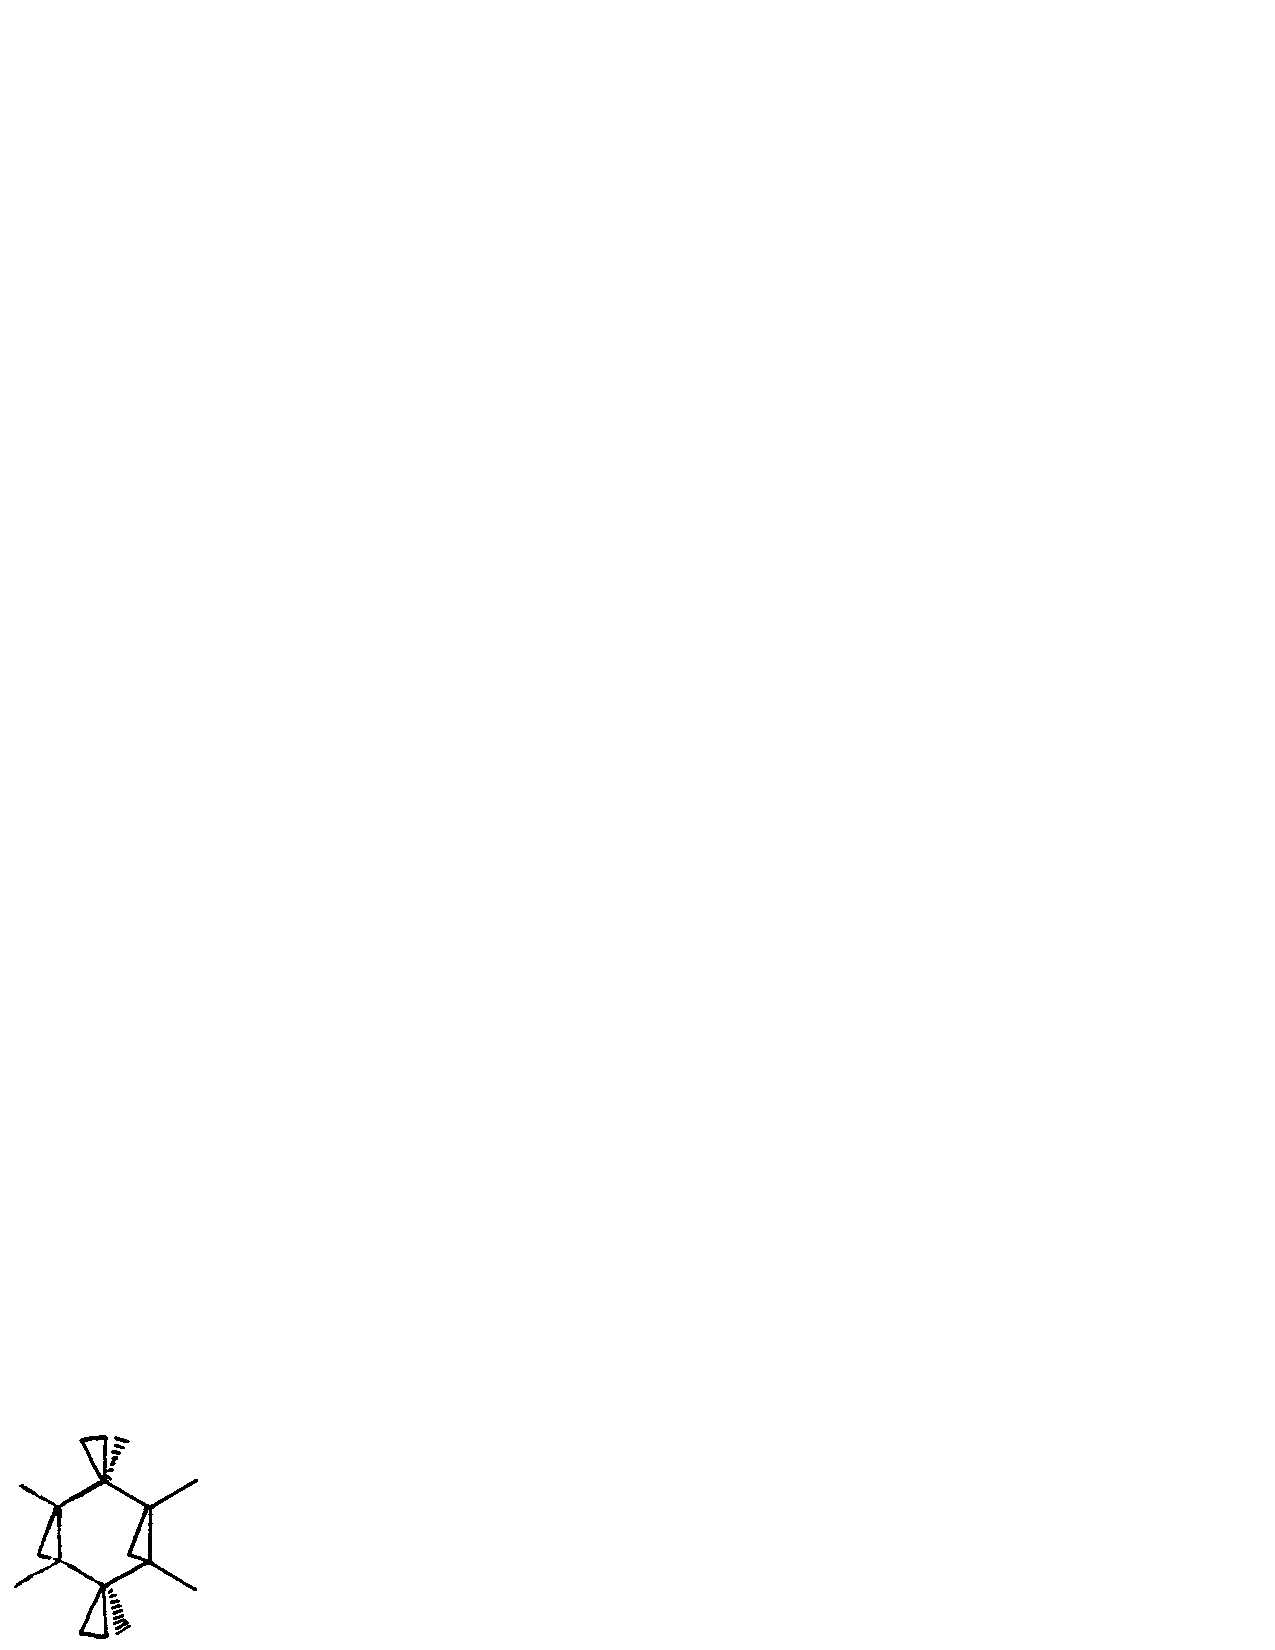
\includegraphics{fg7-3h}
\label{chap7-eqno12}
\end{equation}
These rings correspond to the chair form of cyclohexane, 
C$_6$H$_{12}$,
\begin{equation}
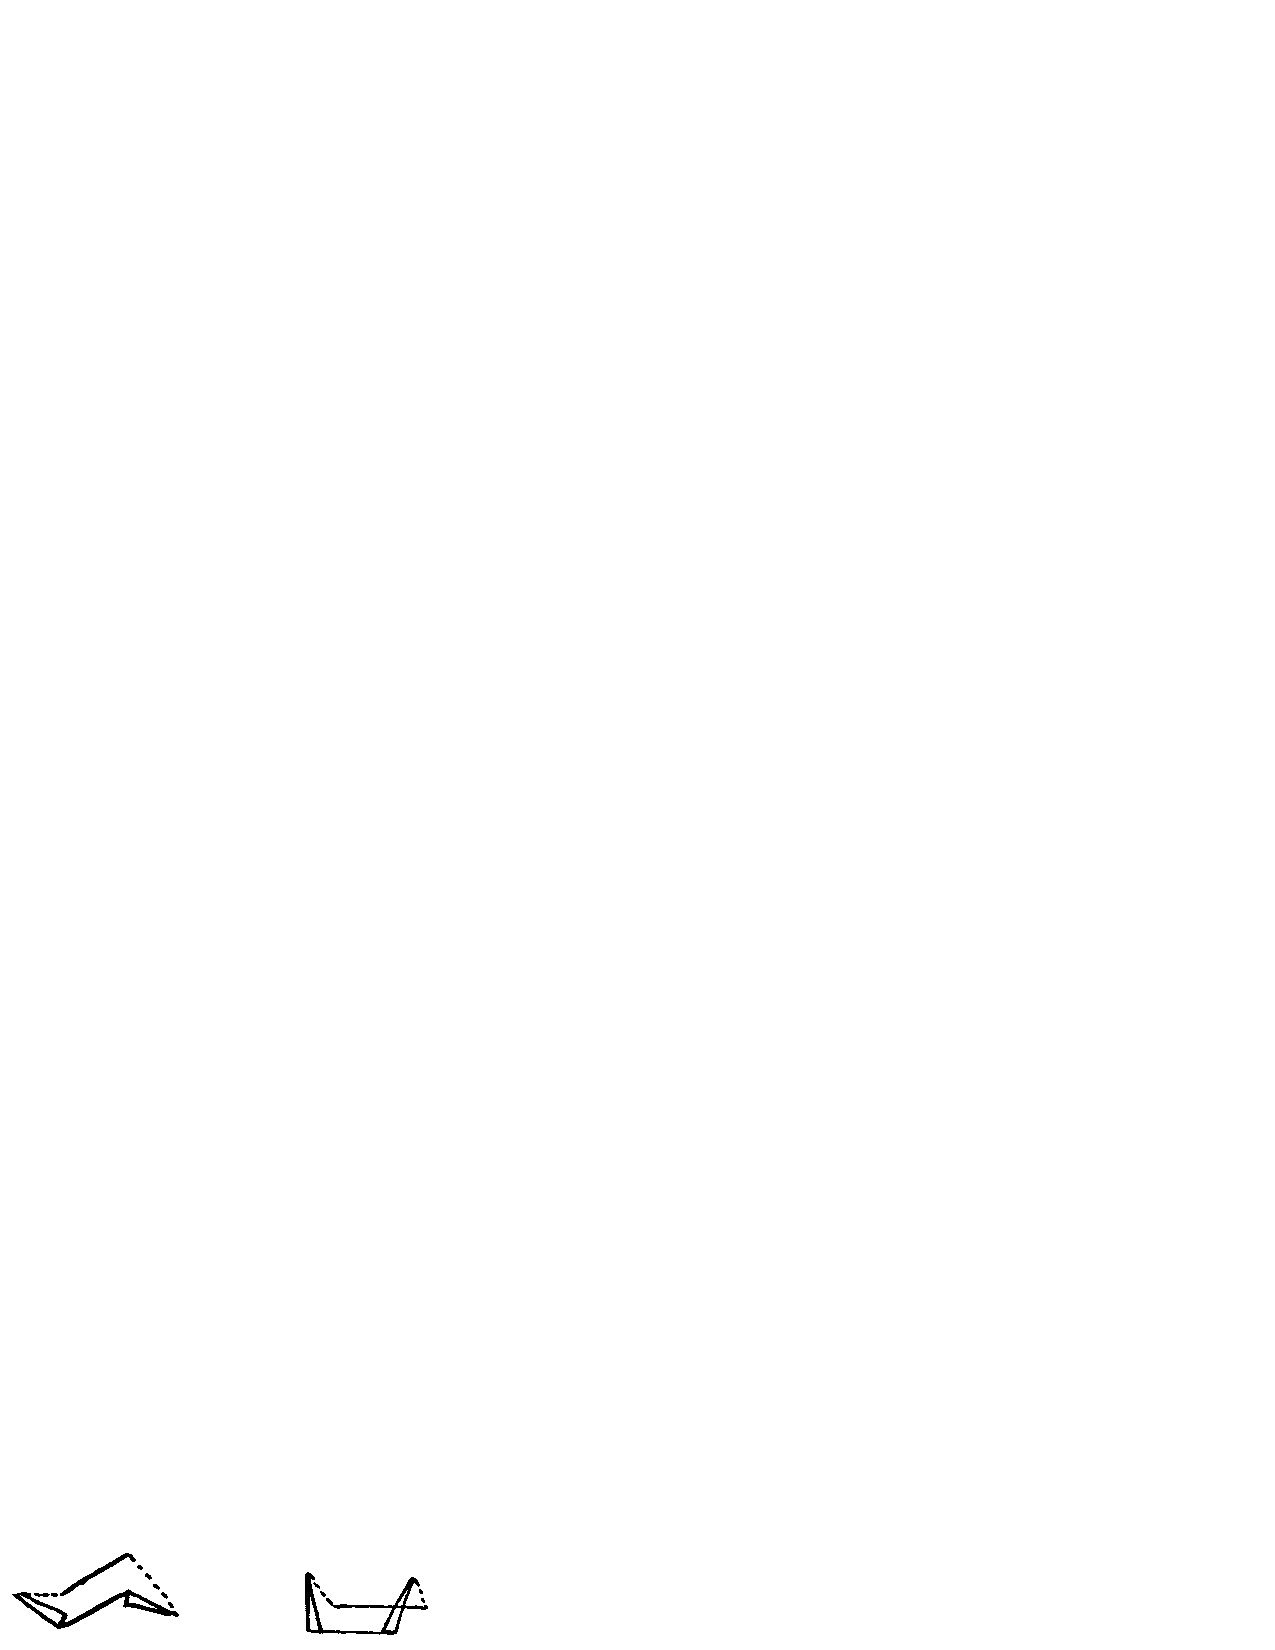
\includegraphics{fg7-3i}
\label{chap7-eqno13}
\end{equation}
\end{enumerate}


\begin{figure}
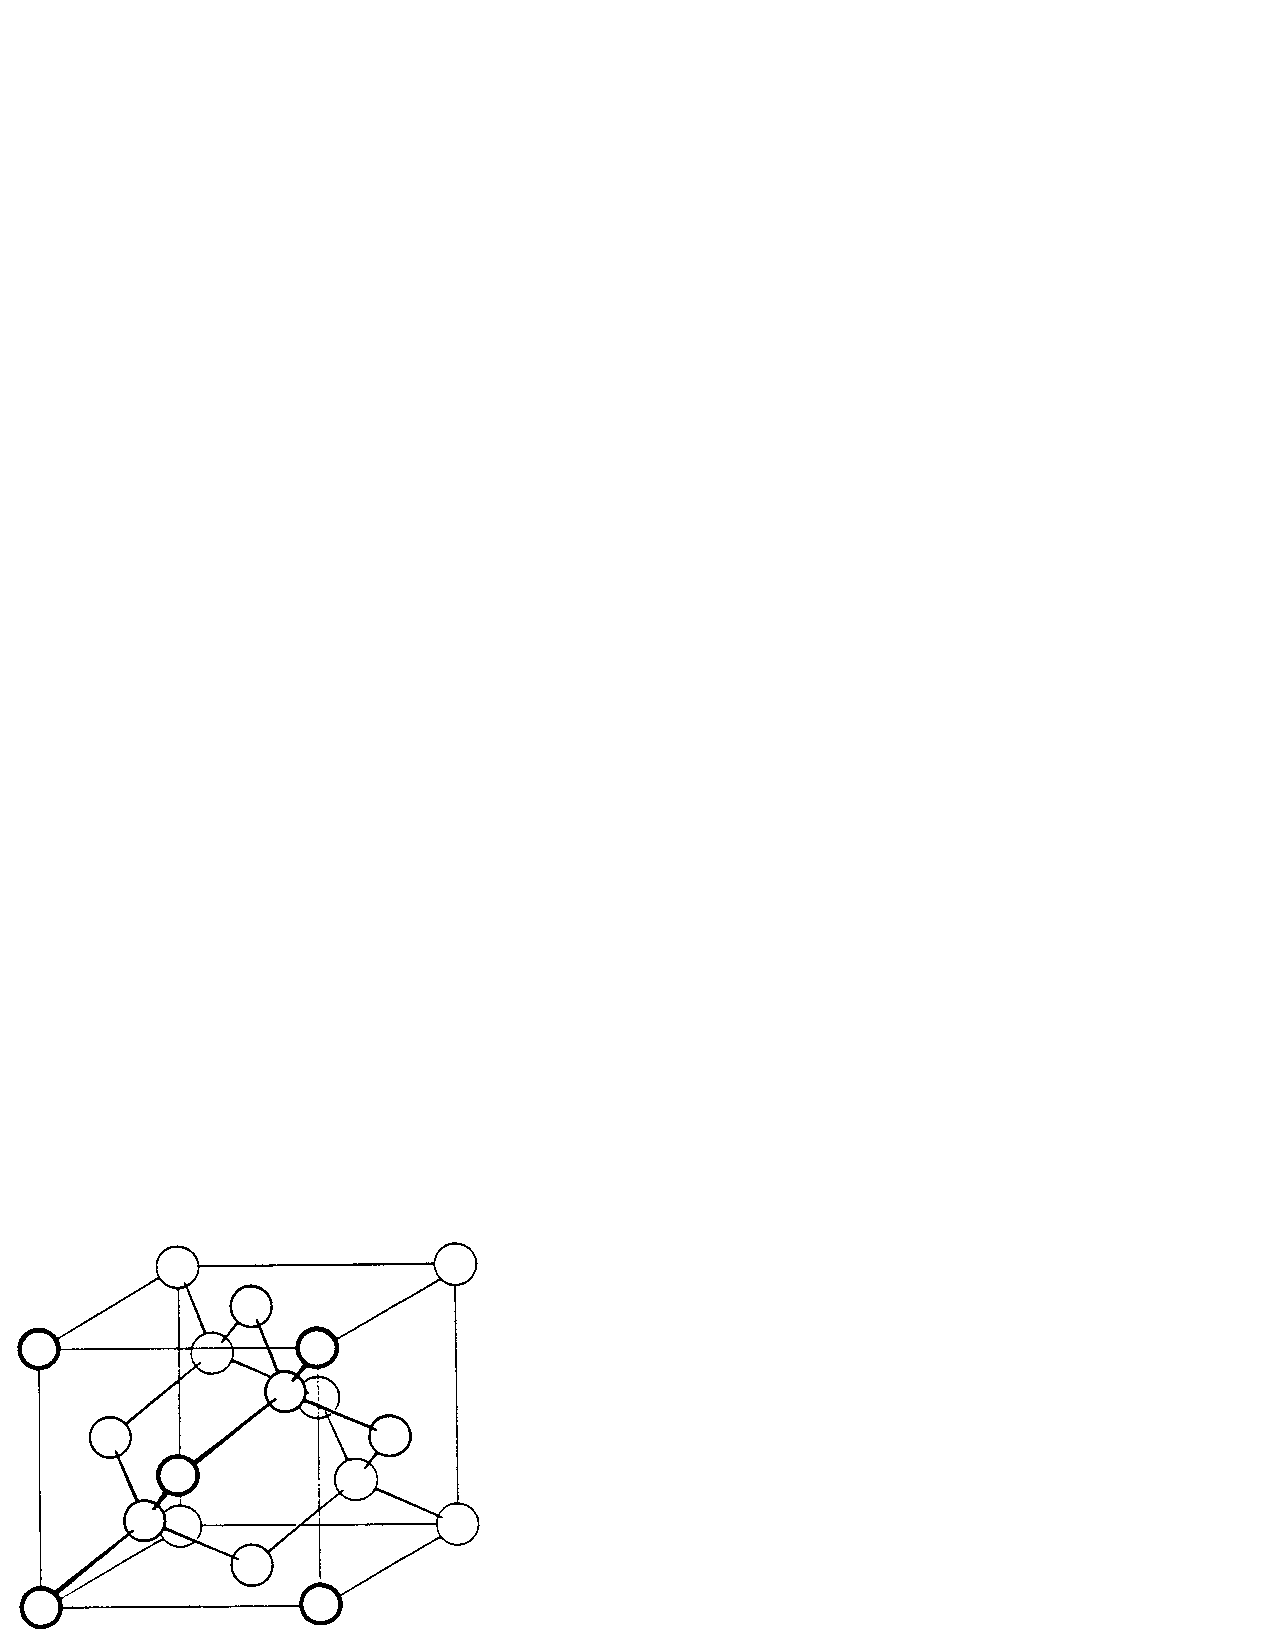
\includegraphics[scale=0.75]{fg7-4}
\caption{The diamond structure: if the side of the cube is 
length $a$, then atoms are at the positions of
(0,0,0), (${1 \over 2}a, {1 \over 2}a,0$), (${1 \over 2}a,0,{1 \over 
2}a$), ($0,{1 \over 2}a, {1 \over 2}a$), (${1 \over 4}a, {1 \over 
4}a, {1 \over 4}a$), (${3 \over 4}a, {3 \over 4}a, {1 \over 4}a$), 
(${3 \over 4}a, {1 \over 4}a, {3 \over 4}a$), and (${1 \over 4}a, {3 
\over 4}a, {3 \over 4}a$).  All other positions obtained by adding or 
subtracting an integer number times $a$ to any of these coordinates.}
\label{chap7-fig4}
\end{figure}

An alternative view of the diamond structure is in terms of cubes that
can be repeated to fill all space, see Figure \ref{chap7-fig4}.  Here,
there are atoms at the eight corners of the cube, at the six faces of
the cube, and four atoms internal to the cube.  There are not,
however, 18 atoms associated with this cube, only one-eighth of each
corner atom, and one-half of each face atom are inside the cube.
Thus, the number of atoms inside the cube is $8 \times {1 \over 8} + 6
\times {1 \over 2} + 4 = 8$ atoms, and the volume per atom is ${1
\over 8}a^3$.

The C-C bond distance for diamond is 1.5445 \AA, which is slightly
longer than the value 1.526 \AA characteristic of simple alkanes.

\section{Carbon-Carbon Multiple Bonds}

\subsection{Ethylene, Valence Bond Description}

Starting with two methylene radicals (CH$_2$) in the ground state 
($^3$B$_1$)
\begin{equation}
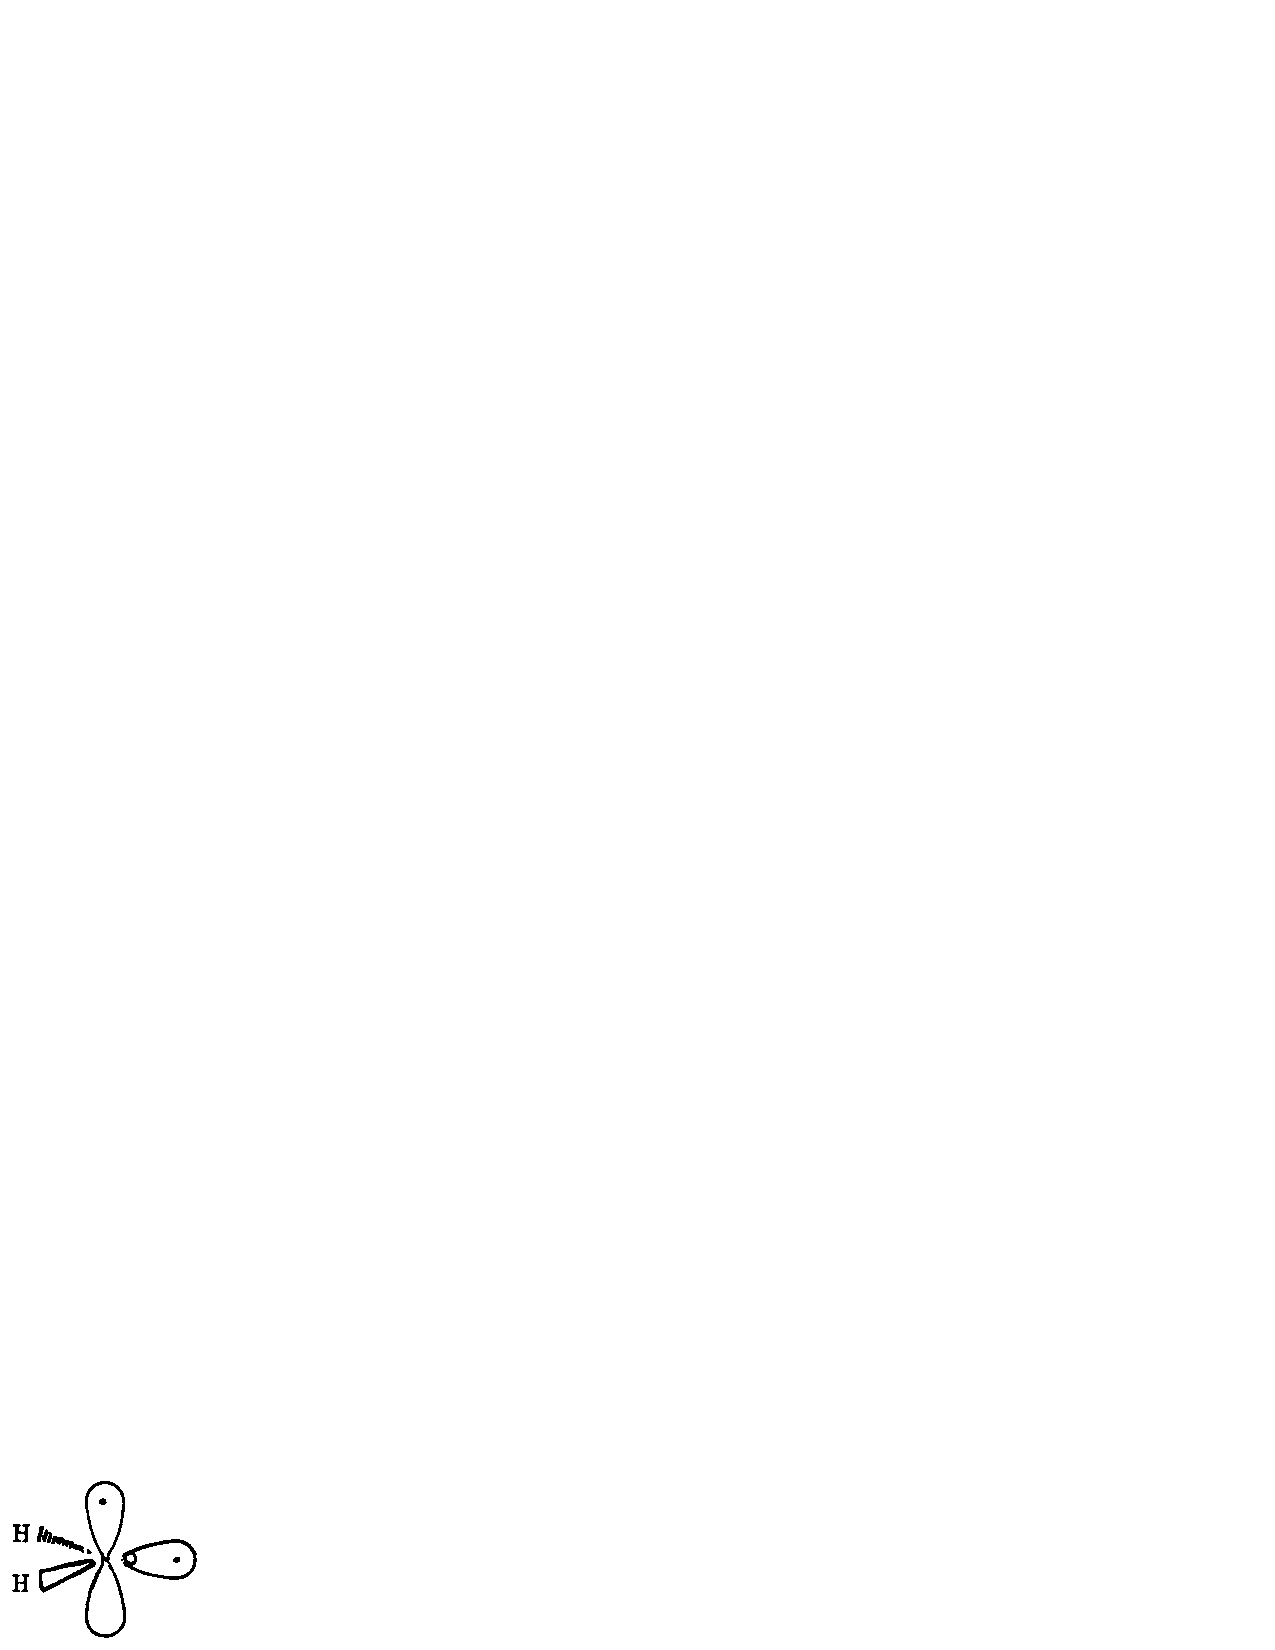
\includegraphics{fg7-4a}
\label{chap7-eqno14}
\end{equation}
and forming ethylene, H$_2$C$=$CH$_2$, we can form both a $\sigma$ bond, and 
a $\pi$ bond, leading to a planar molecule
\begin{equation}
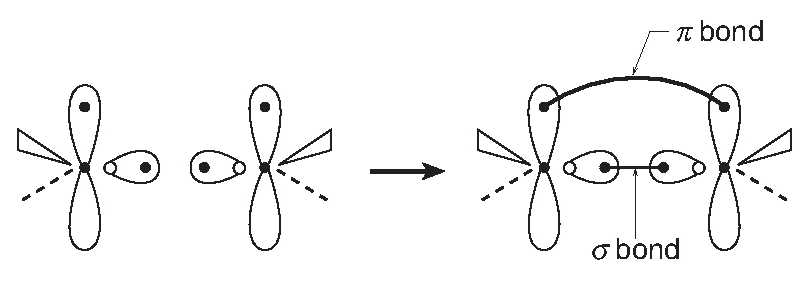
\includegraphics{fg7-4b}
\label{chap7-eqno15}
\end{equation}

In the triplet state of CH$_2$ the HCH bond angle is 132.3$^{\circ}$, but 
forming a bond to the carbon should decrease this angle, because of
Pauli repulsion due to new bond pair.  Thus in CH$_3$ the 
bond angle is decreased to 120$^{\circ}$ and in ethylene,
\begin{equation}
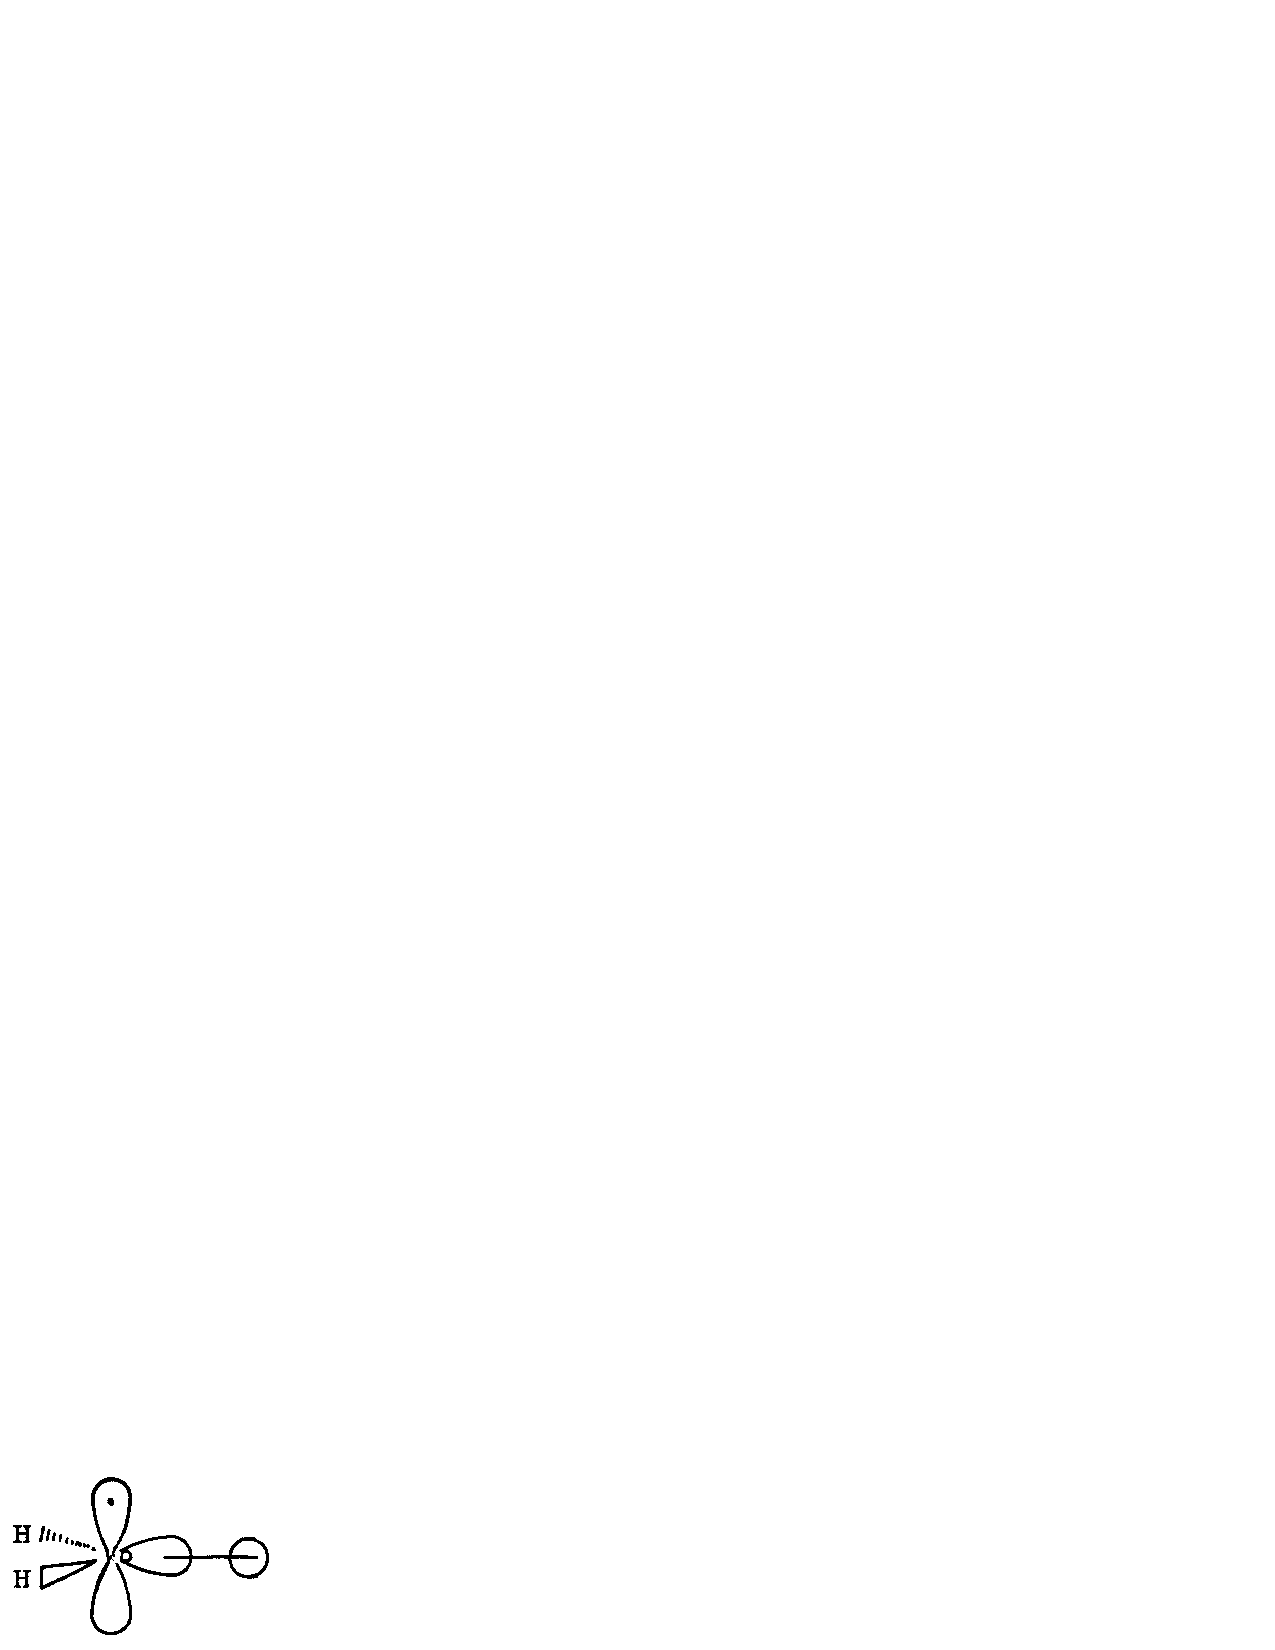
\includegraphics{fg7-4c}
\label{chap7-eqno16}
\end{equation}
the HCH bond angle is decreased further to 117.6$^{\circ}$.

The resulting self-consistent GVB orbitals \cite{chap7-ref1} of
ethylene are shown in Figure \ref{chap7-fig5}, compared with the
orbitals of CH$_2$ ($^3$B$_1$) in Figure \ref{chap7-fig6}.


\begin{figure}
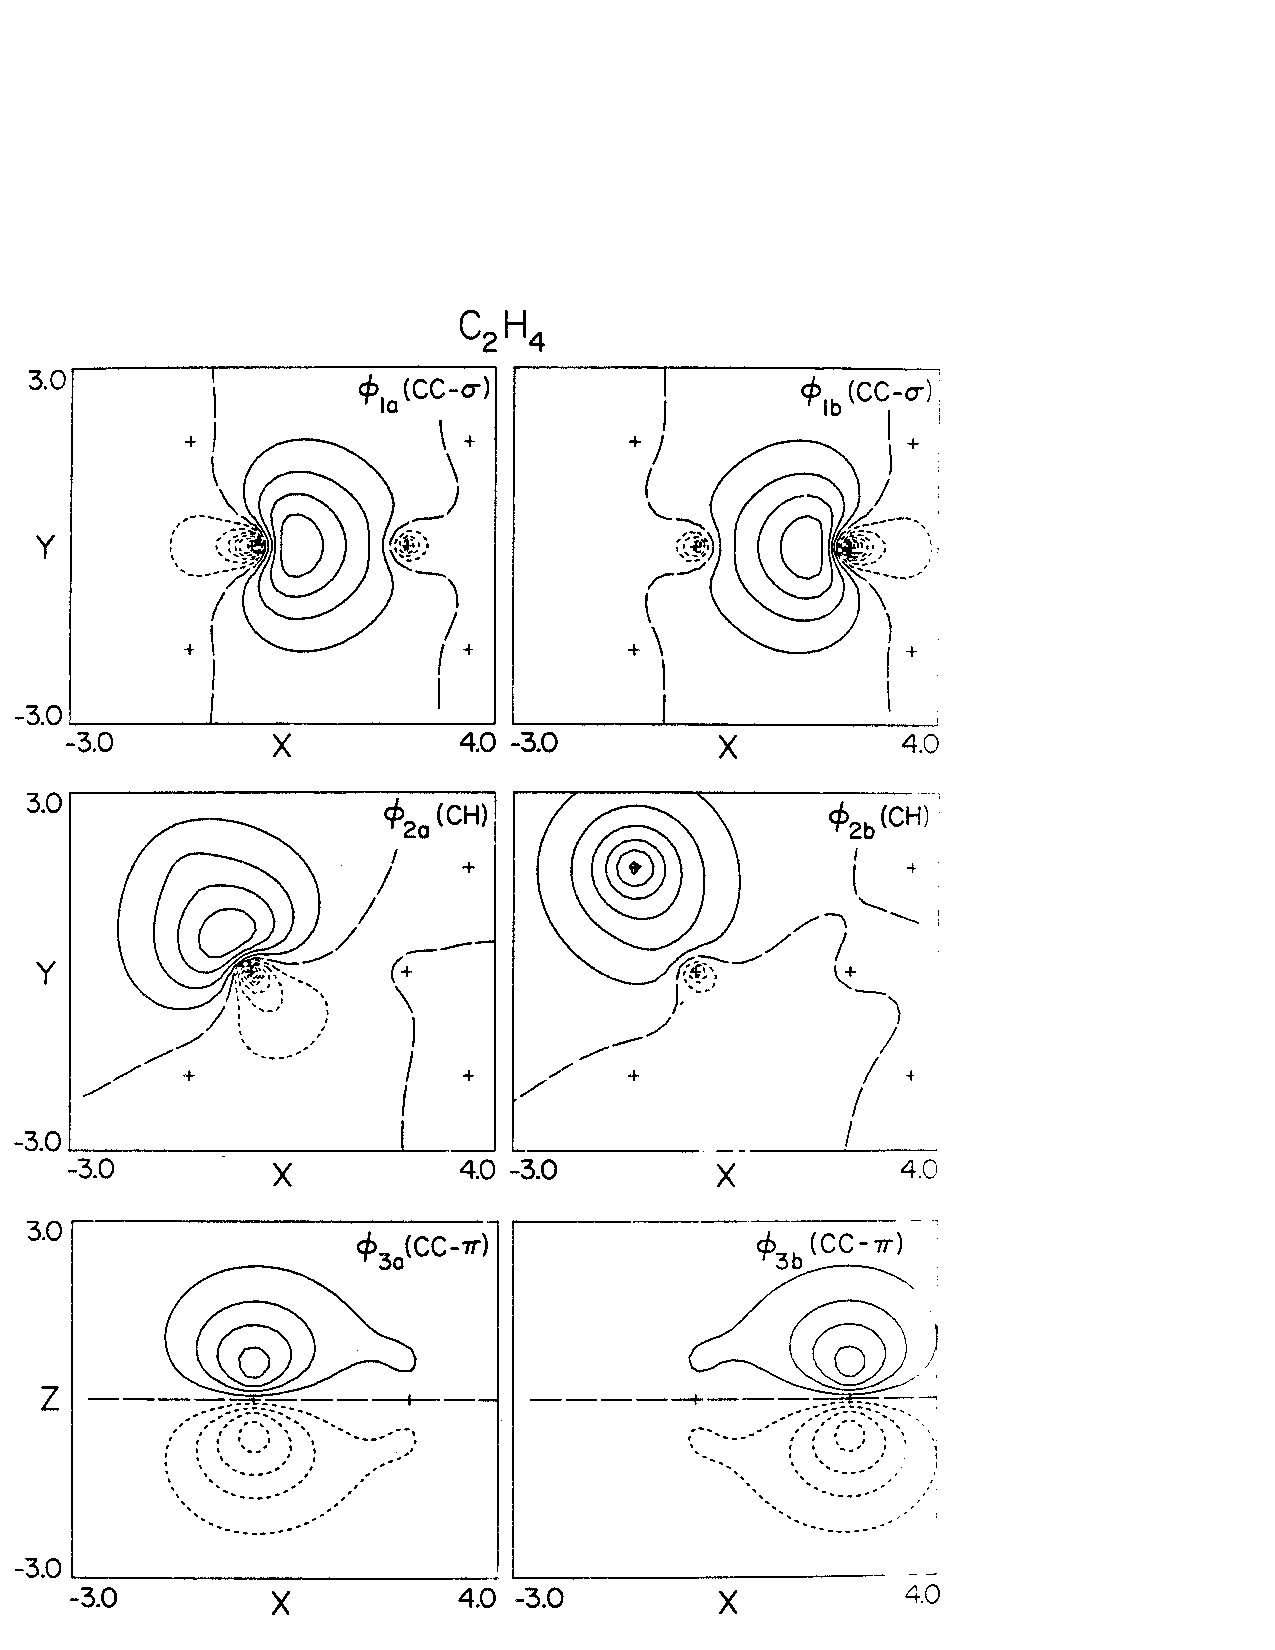
\includegraphics[scale=0.75]{fg7-5}
\caption{C$_2$H$_4$}
\label{chap7-fig5}
\end{figure}


\begin{figure}
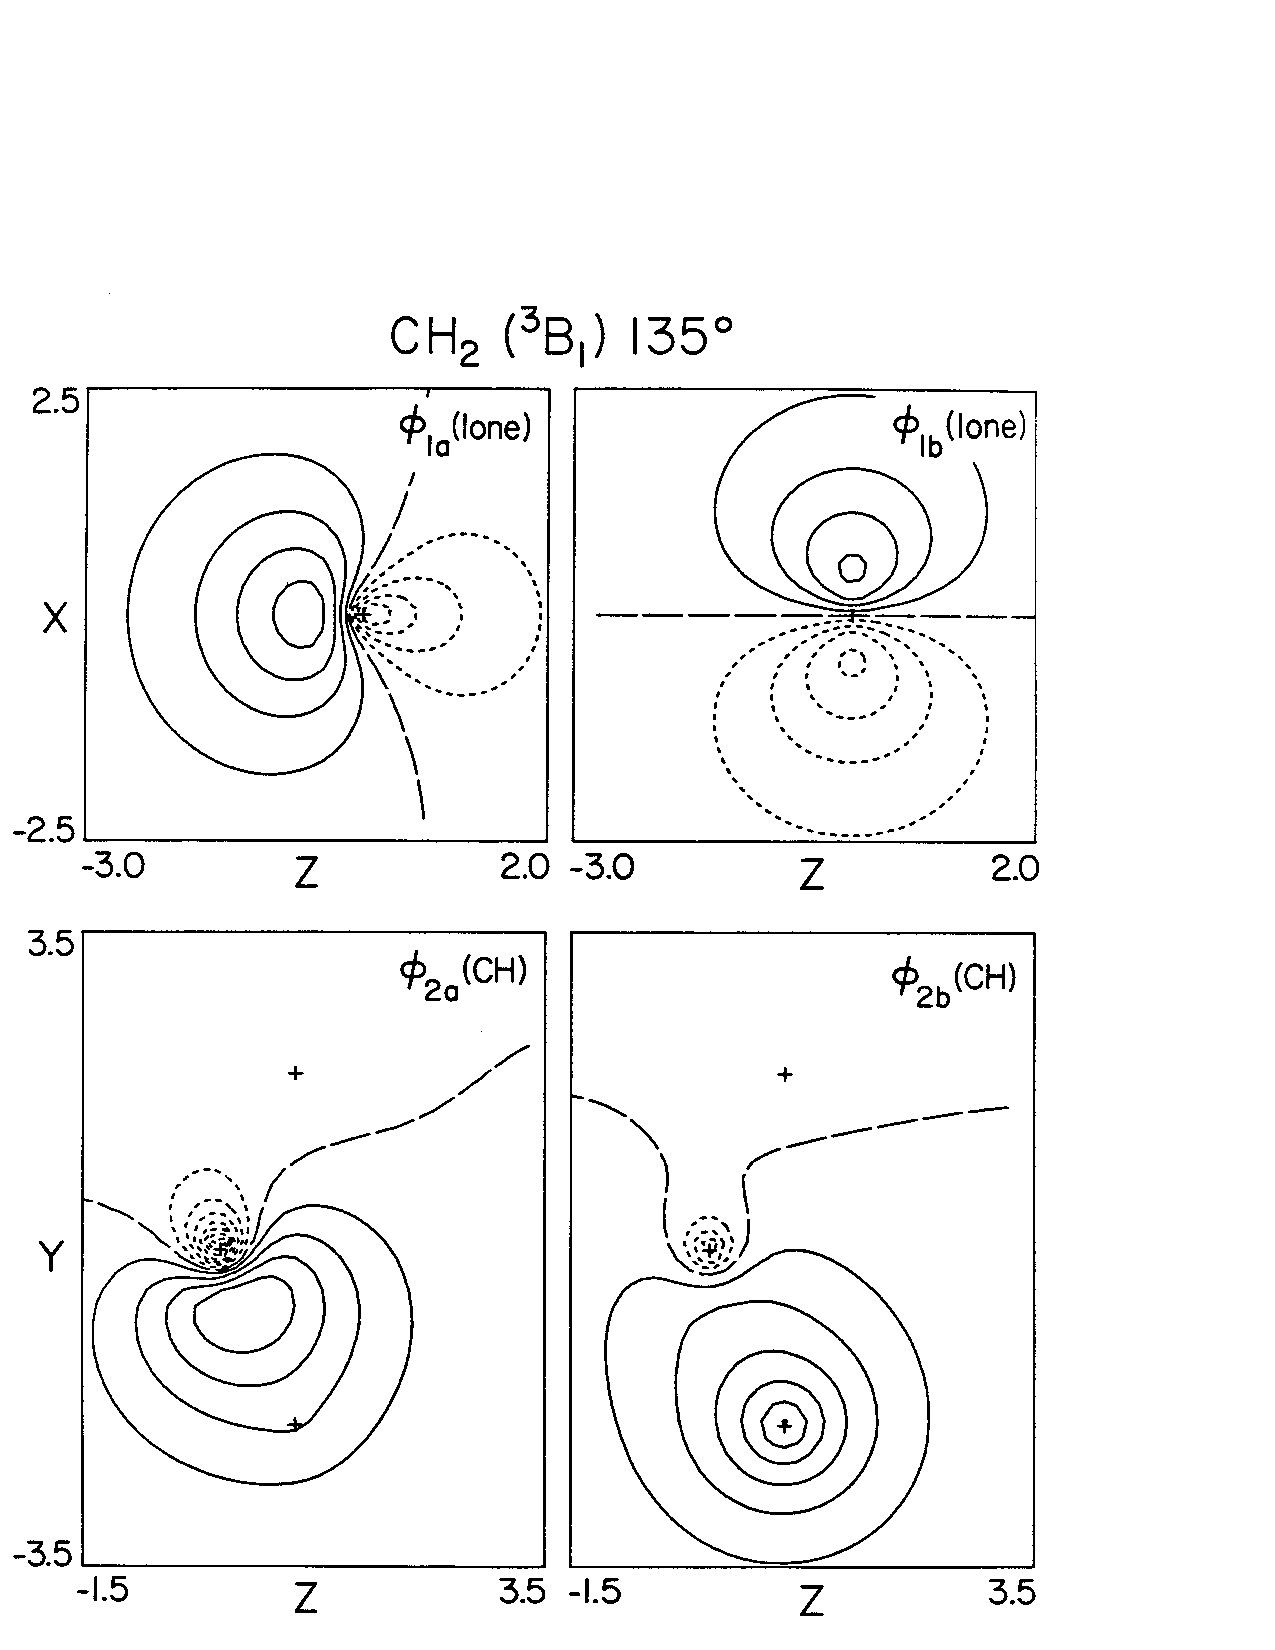
\includegraphics[scale=0.75]{fg7-6}
\caption{CH$_2$($^3$B$)_1$ at 135$^{\circ}$.}
\label{chap7-fig6}
\end{figure}

Consider now the case where the plane of one methylene group is
rotated by an angle of 90$^{\circ}$ with respect to the other, about
the CC axis.  In this case, (\ref{chap7-eqno2}) becomes
\begin{equation}
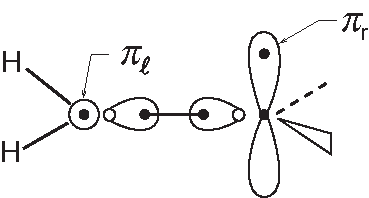
\includegraphics{fg7-6a}
\end{equation}
so that only the $\sigma$ bond is formed.  The nonbonding orbitals 
$\pi_{\ell}$ and $\pi_r$ can be combined into singlet and triplet states:
\begin{equation}
{\rm singlet:} ~ \psi_N = \left( \pi_{\ell} \pi_r + \pi_r \pi_{\ell} 
\right) \left( \alpha \beta - \beta \alpha \right) N ~ state
\label{chap07-eqno17}
\end{equation}
\begin{equation}
{\rm triplet:} ~ \psi_T = \left( \pi_{\ell} \pi_r - \pi_r \pi_{\ell} 
\right) \left( \alpha \beta + \beta \alpha \right) T ~ state
\label{chap07-eqno18}
\end{equation}
where the singlet state is referred to as $N$, for normal or ground 
state, and the triplet state is referred to as $T$.  Based on Hund's 
rule, we would expect the $T$ state to be slightly lower than the 
$N$ state, for 90$^{\circ}$ twist.  However, since these orbitals are 
localized on different centers, the energy splitting should 
be quite small, approximately 1.4 kcal.  In fact, other small effects 
lead to the $N$ state at 90$^{\circ}$ being 
about 1 kcal below the $T$ state.  This is explained in the Appendix, 
however, for our purposes it is only important that these states 
are nearly degenerate.

Comparing the energies of twisted and planar ethylene, leads to the
results in Figure \ref{chap7-fig7}. Thus, the singlet state prefers
planar geometry since the overlap of the $\pi_{\ell}$ and $\pi_r$
orbitals leads to a strong $\pi$ bond.  However, for the triplet
state, the $\pi_{\ell}$ and $\pi_r$ orbitals must be orthogonalized to
each other, and hence, this state prefers the 90$^{\circ}$ twisted
geometry.

\begin{figure}
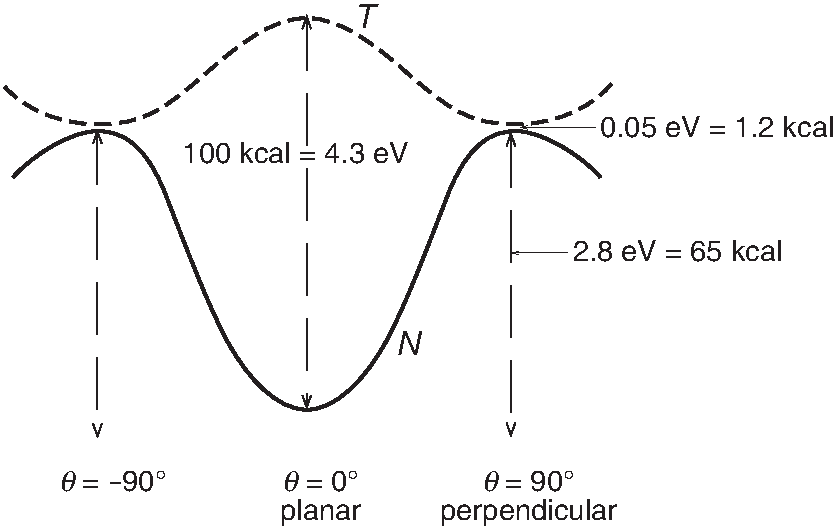
\includegraphics[scale=0.75]{fg7-7}
\caption{}
\label{chap7-fig7}
\end{figure}


\subsection{The Rotational Barrier}

According to Figure \ref{chap7-fig7} the energy to twist, $N$ state,
ethylene by 90$^{\circ}$ is 65 kcal, breaking the $\pi$ bond.  This
barrier has been observed experimentally$^2$ by studying the kinetics
for cis-trans isomerization, of
\begin{equation}
% missing figure cis-trans isomerization, p7-14
\end{equation}

As the molecules is rotated, the strength of the $\pi$ bond is 
weakened, and the CC bond length increases.  Thus, for the $N$ state
CC = 1.34 \AA\ at $\theta = 0^{\circ}$, and 1.50 \AA\ at 
$\theta = 90^{\circ}$.

In the $T$ state, the optimum geometry is twisted, $\theta =
90^{\circ}$, since triplet pairing of the orbitals prefers $S = 0$.
As the molecule is twisted toward the planar geometry the bond length
increases from CC = 1.50 \AA\ at $\theta = 90^{\circ}$ to 1.57 \AA\ at
$\theta = 0^{\circ}$, and the energy barrier is 25 kcal.  Note that in
Figure \ref{chap7-fig7} we show the $T$ to $N$ energy separation at
$\theta = 0$, using the ground state geometry; the adiabatic
excitation energy for $\theta = 0^{\circ}$ is 91 kcal.

\subsection{Ethylene, Molecular Orbital Description}

In the MO description of ethylene there are two 
$\pi$ MOs
\begin{eqnarray}
\pi_u &= {(\pi_{\ell} + \pi_r) \over \sqrt{2(1+s)}}  ~{\rm bonding}\cr
\pi_g &= {(\pi_{\ell} + \pi_r) \over \sqrt{2(1+s)}}  ~{\rm antibonding}
\label{chap07-eqno19}
\end{eqnarray}
Thus, in the molecular orbital description, the ground state is
\begin{equation}
N : \pi_u \pi_u \left( \alpha \beta - \beta \alpha \right)
\label{chap07-eqno20}
\end{equation}
and the lowest excited states
\begin{equation}
T : \left( \pi_u \pi_g - \pi_g \pi_u \right) \left( \alpha \beta + 
\beta \alpha \right)
\label{chap07-eqno21}
\end{equation}
\begin{equation}
V : \left( \pi_u \pi_g + \pi_g \pi_u \right) \left( \alpha \beta - 
\beta \alpha \right)
\label{chap07-eqno22}
\end{equation}
are obtained by the excitation $\pi_u \rightarrow \pi_g$ from the 
ground state.  There is also an additional state,
\begin{equation}
Z : \pi_g \pi_g \left( \alpha \beta-\beta \alpha \right)
\end{equation}
but it is much higher, and will not be considered here.

First, we consider the $T$ and $V$ excited states. The energies are
\begin{eqnarray}
E_T &=& E_0 - K_{gu}\cr
E_V &=& E_0 + K_{gu}
\label{chap07-eqno23}
\end{eqnarray}
where, from Hund's rule, the $V$ state is higher, by $2K_{gu}$.

The first question is why the valence bond description did not have a
$V$ state. Substituting (\ref{chap7-eqno12}) into
(\ref{chap7-eqno15}), we find
\begin{equation}
\left( \pi_u \pi_g + \pi_g \pi_u \right) = \pi_{\ell} \pi_{\ell} - 
\pi_r \pi_r
\end{equation}
where a normalization term is deleted.  Thus, the $V$ state is an 
ionic wavefunction in which both $\pi$ electrons are either on the left 
or both on the right, but combined to a net wavefunction for which 
both $C$ are equivalent.  In the valence bond description, we obtain 
two covalent states
\begin{equation}
N : \pi_{\ell} \pi_r + \pi_r \pi_{\ell}
\label{chap07-eqno24}
\end{equation}
\begin{equation}
T : \left( \pi_{\ell} \pi_r - \pi_r \pi_{\ell} \right) = \pi_g 
\pi_u - \pi_u \pi_g
\label{chap07-eqno25}
\end{equation}
and two ionic states
\begin{equation}
V : \pi_{\ell} \pi_{\ell} - \pi_r \pi_r = \pi_g \pi_u + \pi_u 
\pi_g
\label{chap07-eqno26}
\end{equation}
\begin{equation}
Z : \pi_{\ell} \pi_{\ell} + \pi_r \pi_r
\label{chap07-eqno27}
\end{equation}
The wavefunction (\ref{chap7-eqno20}) for $Z$ has a high overlap with
the wavefunction for the $N$ state.  The real wavefunction for the
excited state must be orthogonal to $N$ leading to a very high energy
for $Z$.  Thus, the molecular orbital and valence bond description of
the $T$ and $V$ states are equivalent. They differ for the $N$ state
since
\begin{equation}
\pi_u \pi_u = \left( \pi_{\ell} \pi_r + \pi_r \pi_{\ell} \right) + 
\left( \pi_{\ell} \pi_{\ell} - \pi_r \pi_r \right),
\label{chap07-eqno28}
\end{equation}
where $(\pi_{\ell} \pi_r + \pi_r \pi_{\ell})$ is the covalent, and 
$(\pi_{\ell} \pi_{\ell} - \pi_r \pi_r)$ is the ionic.  Thus, 
the molecular orbital wavefunction forces equal ionic and covalent 
character.  Alternatively, the generalized valence bond wavefunction 
may be written as
\begin{equation}
\left( \pi_{\ell} \pi_{\ell} + \pi_r \pi_r \right) = C_1 \pi_u 
\pi_u - C_2 \pi_g \pi_g
\label{chap07-eqno29}
\end{equation}
indicating that the dominant electron correlation terms are included.

\subsection{Carbon-Carbon Triple Bonds}

Starting with two CH radicals, ${^4\Sigma}^-$ state, and forming
acetylene, HC$\equiv$CH, we make a triple bond; that is, a $\sigma$
bond and two $\pi$ bonds
\begin{equation}
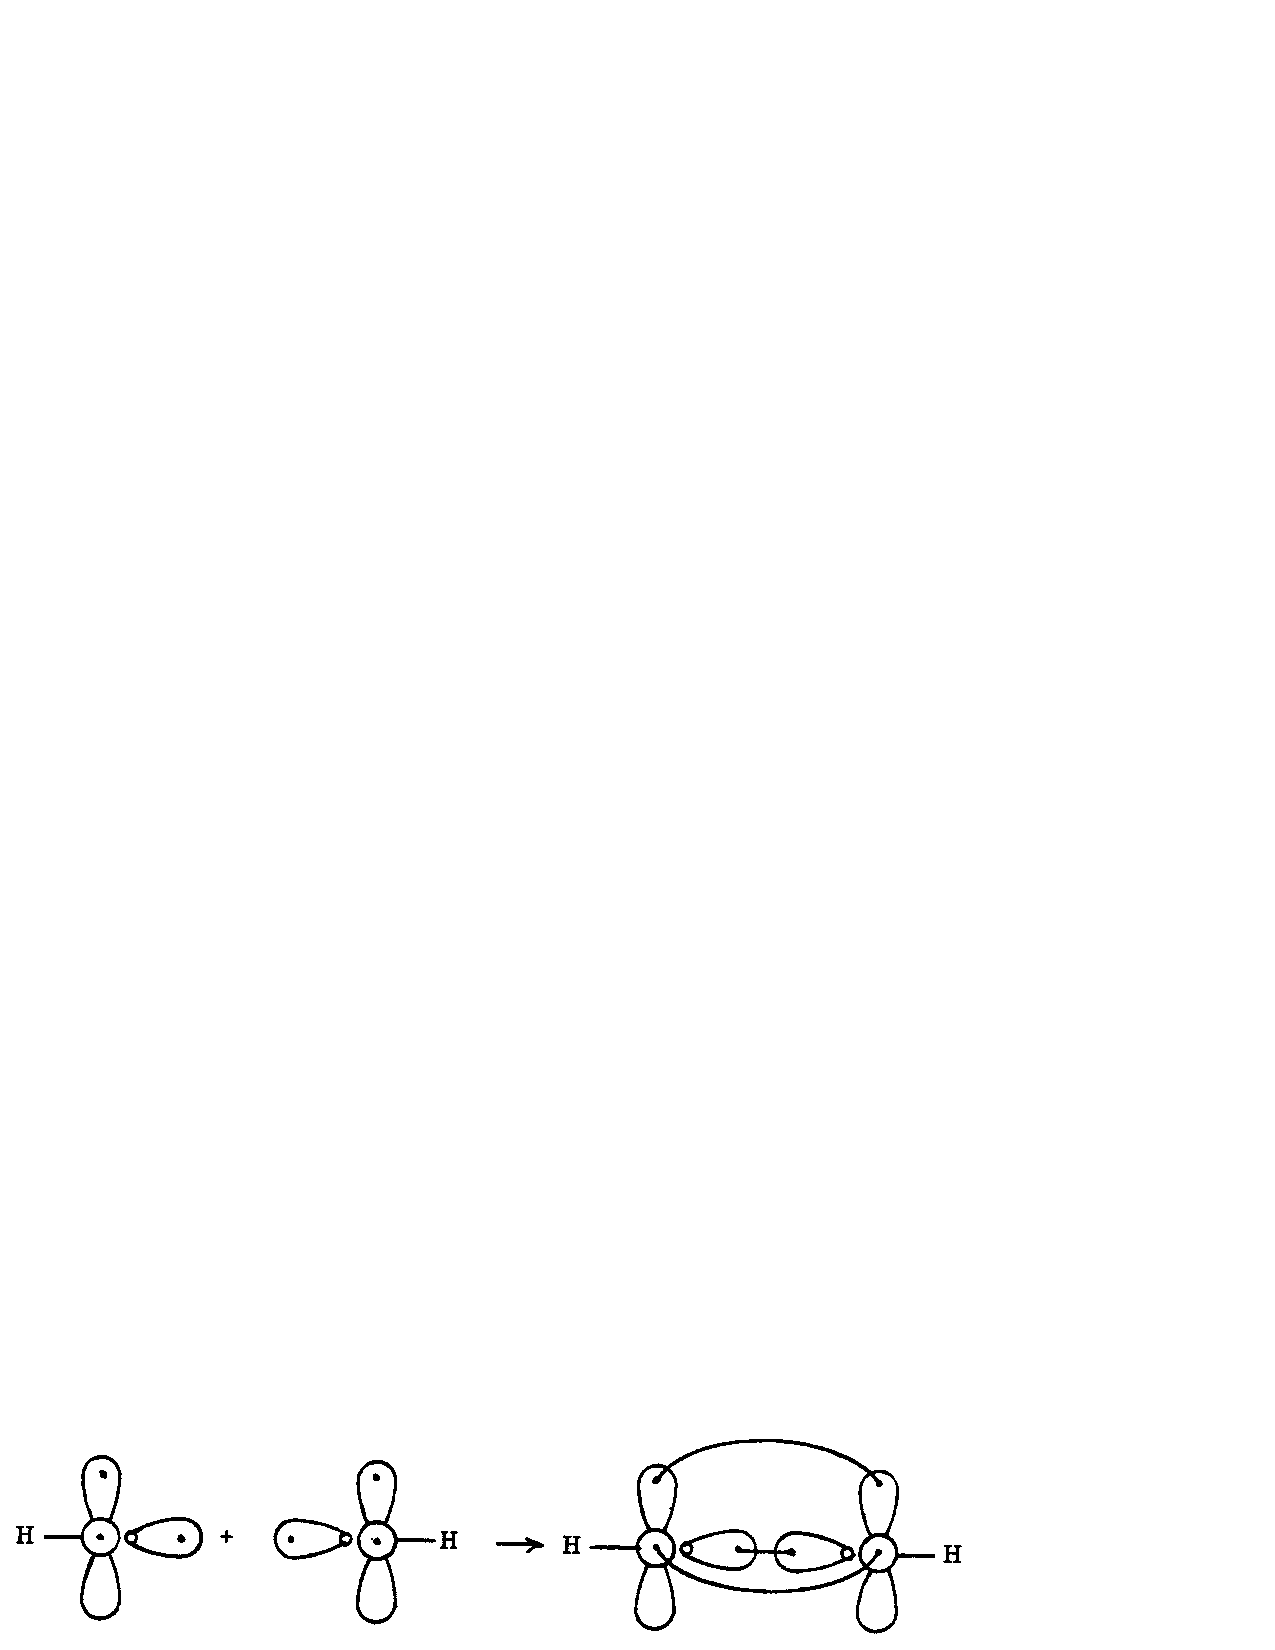
\includegraphics{fg7-7a}
\label{chap7-eqno30}
\end{equation}
There is a problem here, however.  The ground state of CH is the 
${^2\Pi}$ state (top) not the ${^4\Sigma}^-$ state (bottom)
\begin{equation}
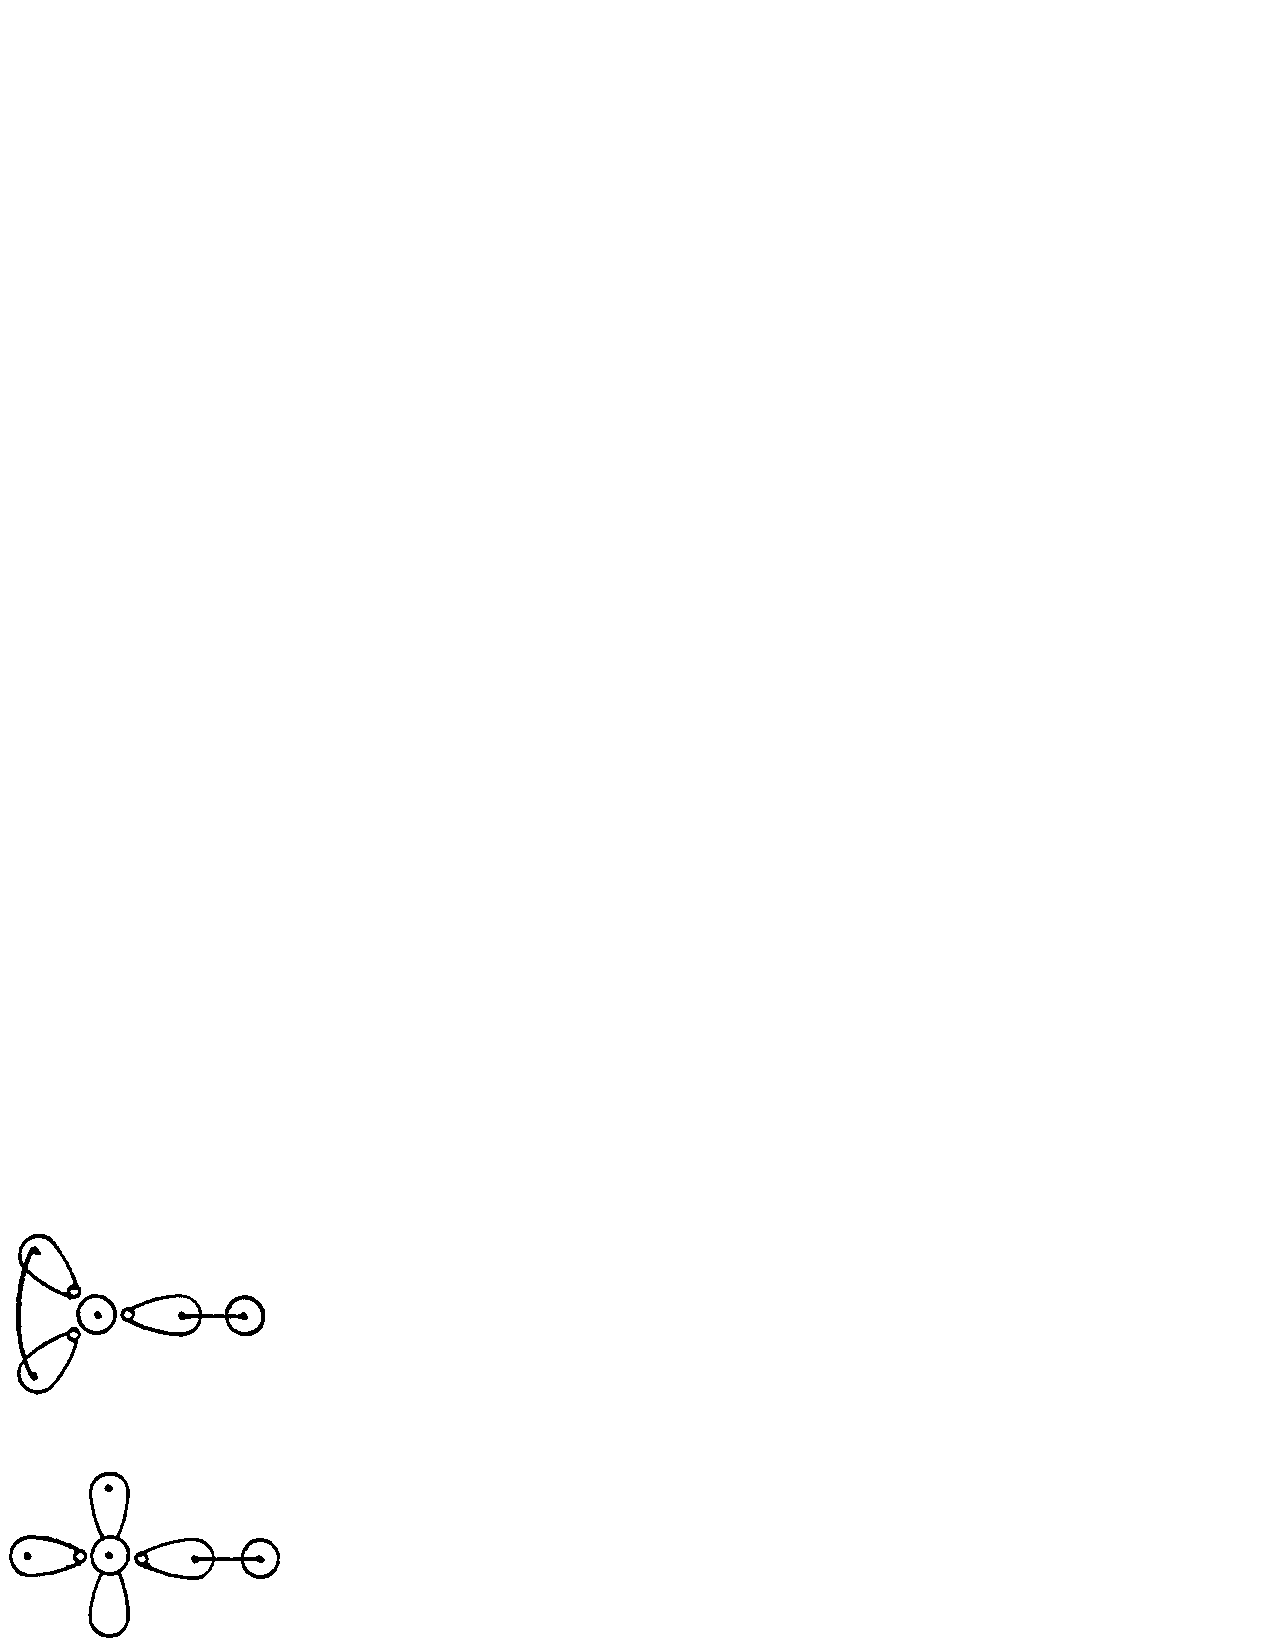
\includegraphics{fg7-7b}
\label{chap7-eqno32}
\end{equation}
shown in (\ref{chap7-eqno30}) and which is related to acetylene.
Thus, in making the triple bond, we must promote each CH from the
${^2\Pi}$ to the ${^4\Sigma}^-$ state at a cost of 17 kcal each.  As a
result, the triple bond is 34 kcal weaker than might otherwise have
been expected.

The self-consistent generalized valence bond orbitals$^1$ of acetylene
are shown in Figure \ref{chap7-fig8} and compared with those of both
states of CH in Figure \ref{chap7-fig9}.

\begin{figure}
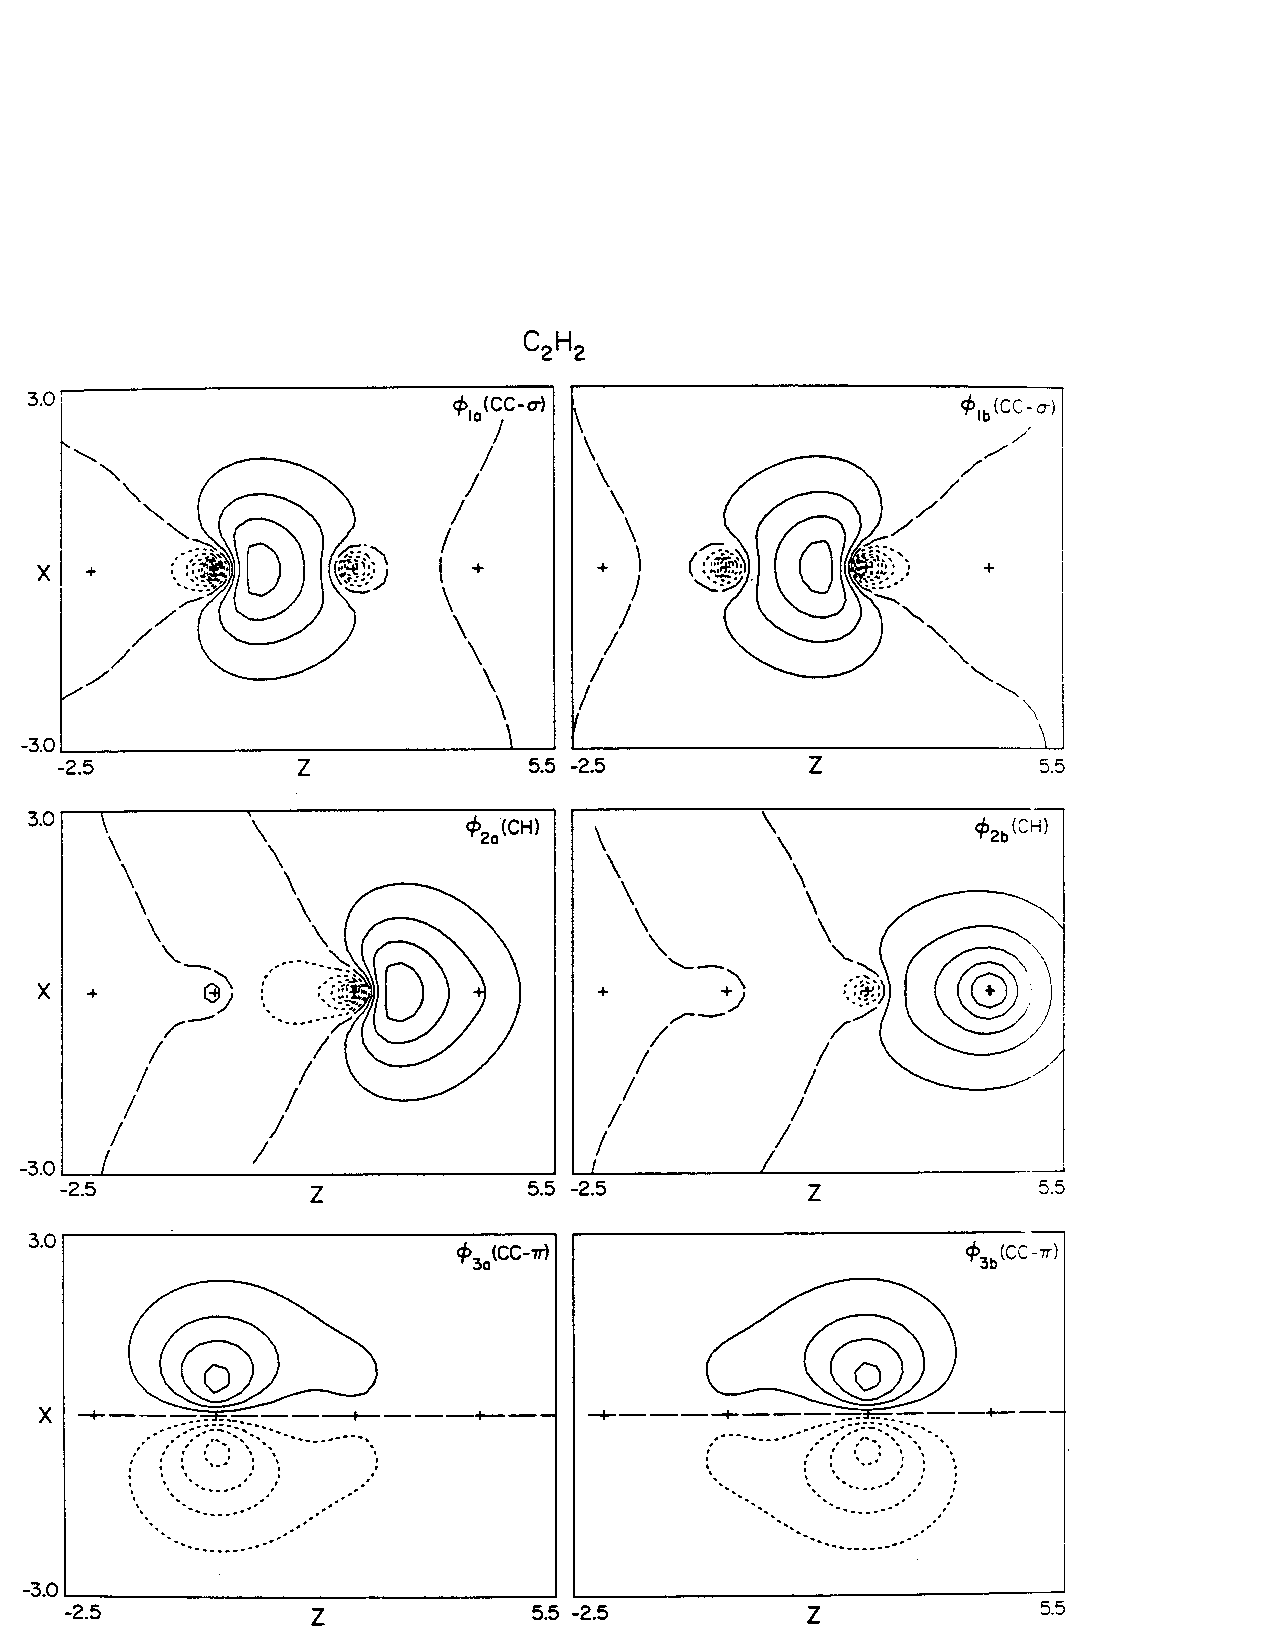
\includegraphics[scale=0.75]{fg7-8}
\caption{C$_2$H$_2$.}
\label{chap7-fig8}
\end{figure}

\begin{figure}
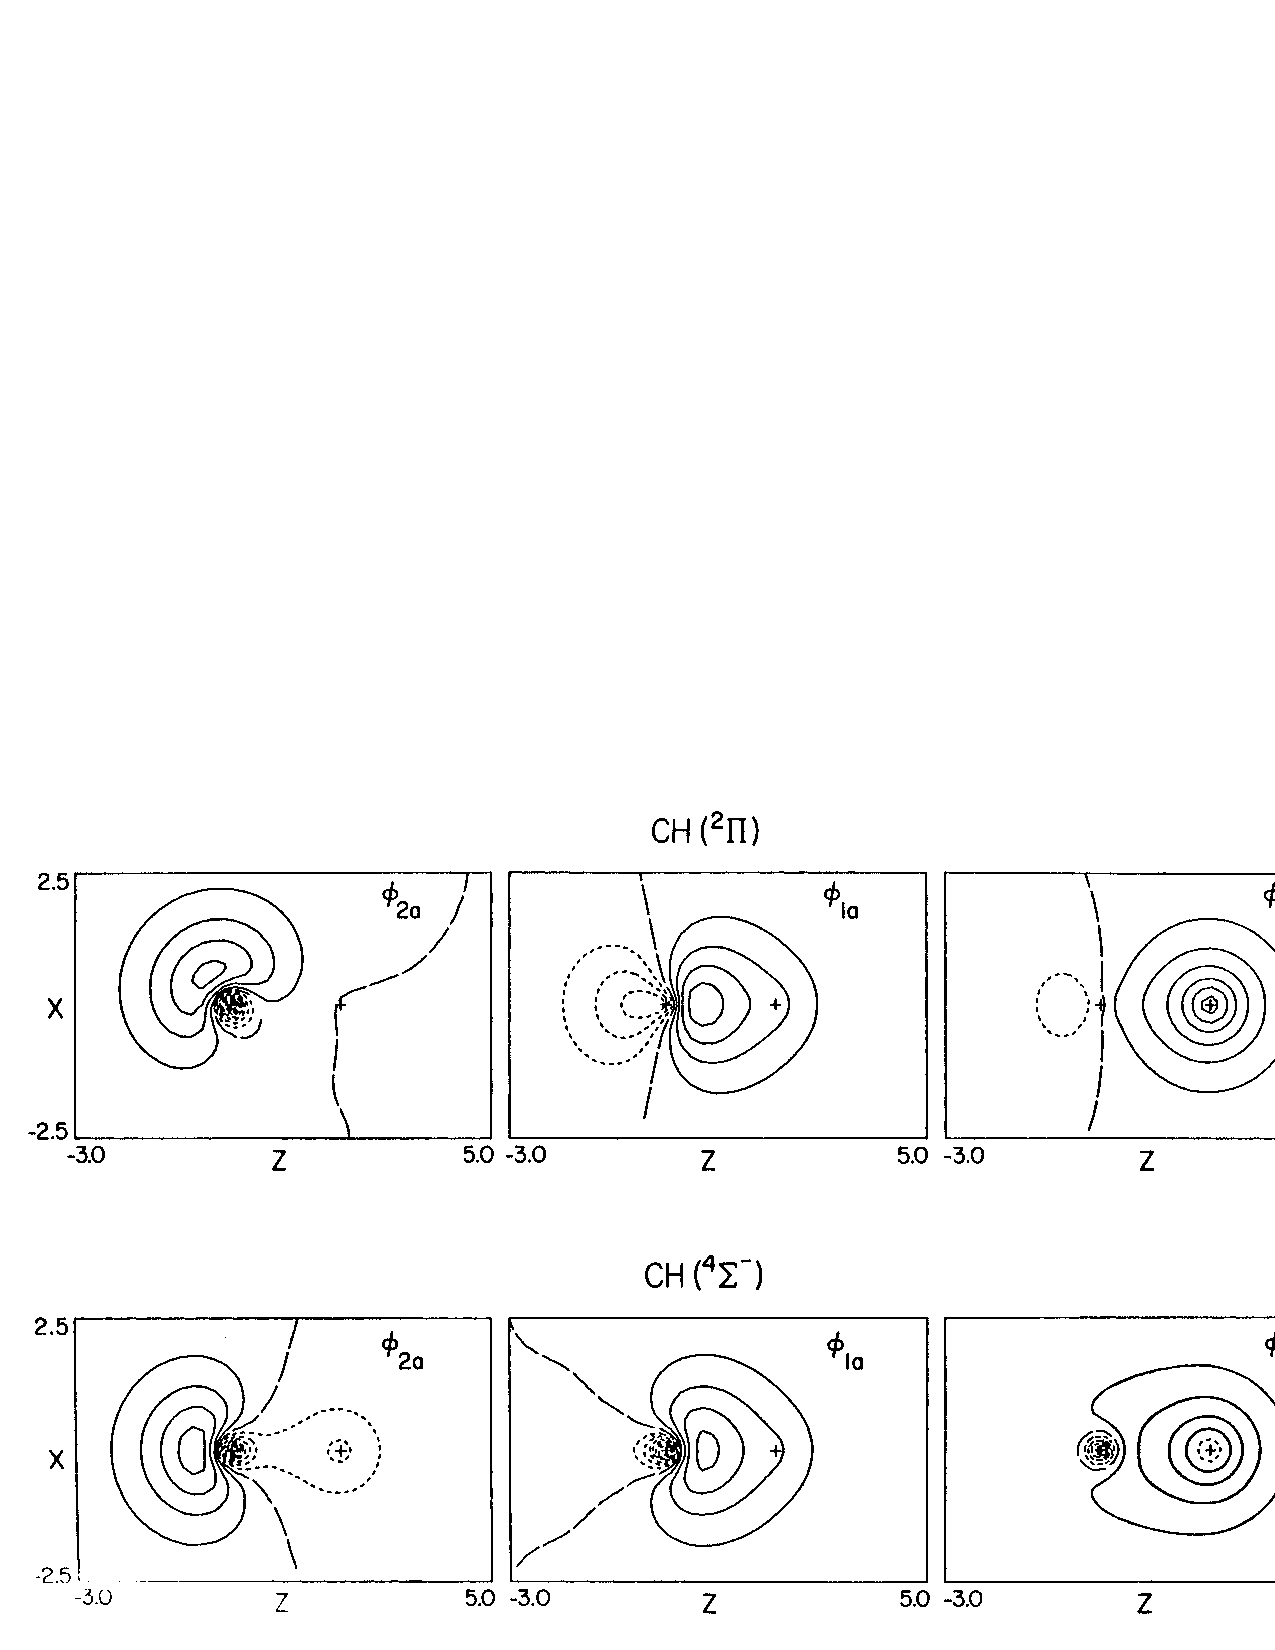
\includegraphics[scale=0.6,angle=90]{fg7-9}
\caption{}
\label{chap7-fig9}
\end{figure}

The molecular orbital description of the $\pi$ system of acetylene 
is $(\pi_{ux})^2(\pi_{uy})^2$ or symbolically $(\pi_u)^4$.
Thus, low-lying excited states would have the configuration of
$(\pi_u)^3(\pi_g)^1$.  This leads to four configurations
\begin{eqnarray}
\left( \pi_{ux} \right)^2 & \left( \pi_{uy} \right)^1 \left( 
\pi_{gx} \right)^1\cr
\left( \pi_{ux} \right)^2 & \left( \pi_{uy} \right)^1 \left( 
\pi_{gy} \right)^1\cr
\left( \pi_{ux} \right)^1 & \left( \pi_{uy} \right)^2 \left( 
\pi_{gx} \right)^1\cr
\left( \pi_{ux} \right)^2 & \left( \pi_{uy} \right)^2 \left( 
\pi_{gy} \right)^1
\label{chap07-eqno33}
\end{eqnarray}
each of which leads to both triplet and singlet states.  Proper analysis of
the symmetry leads to
\begin{equation}
{^3\Sigma}^+_u , {^3\Delta}^-_u , {^3\Sigma}^-_u , {^1\Sigma}^-_u , 
{^1\Delta}_u , {^1\Sigma}^+_u
\label{chap07-eqno34}
\end{equation}
in order of increasing energy.

Consider the geometry of the triplet state
\begin{equation}
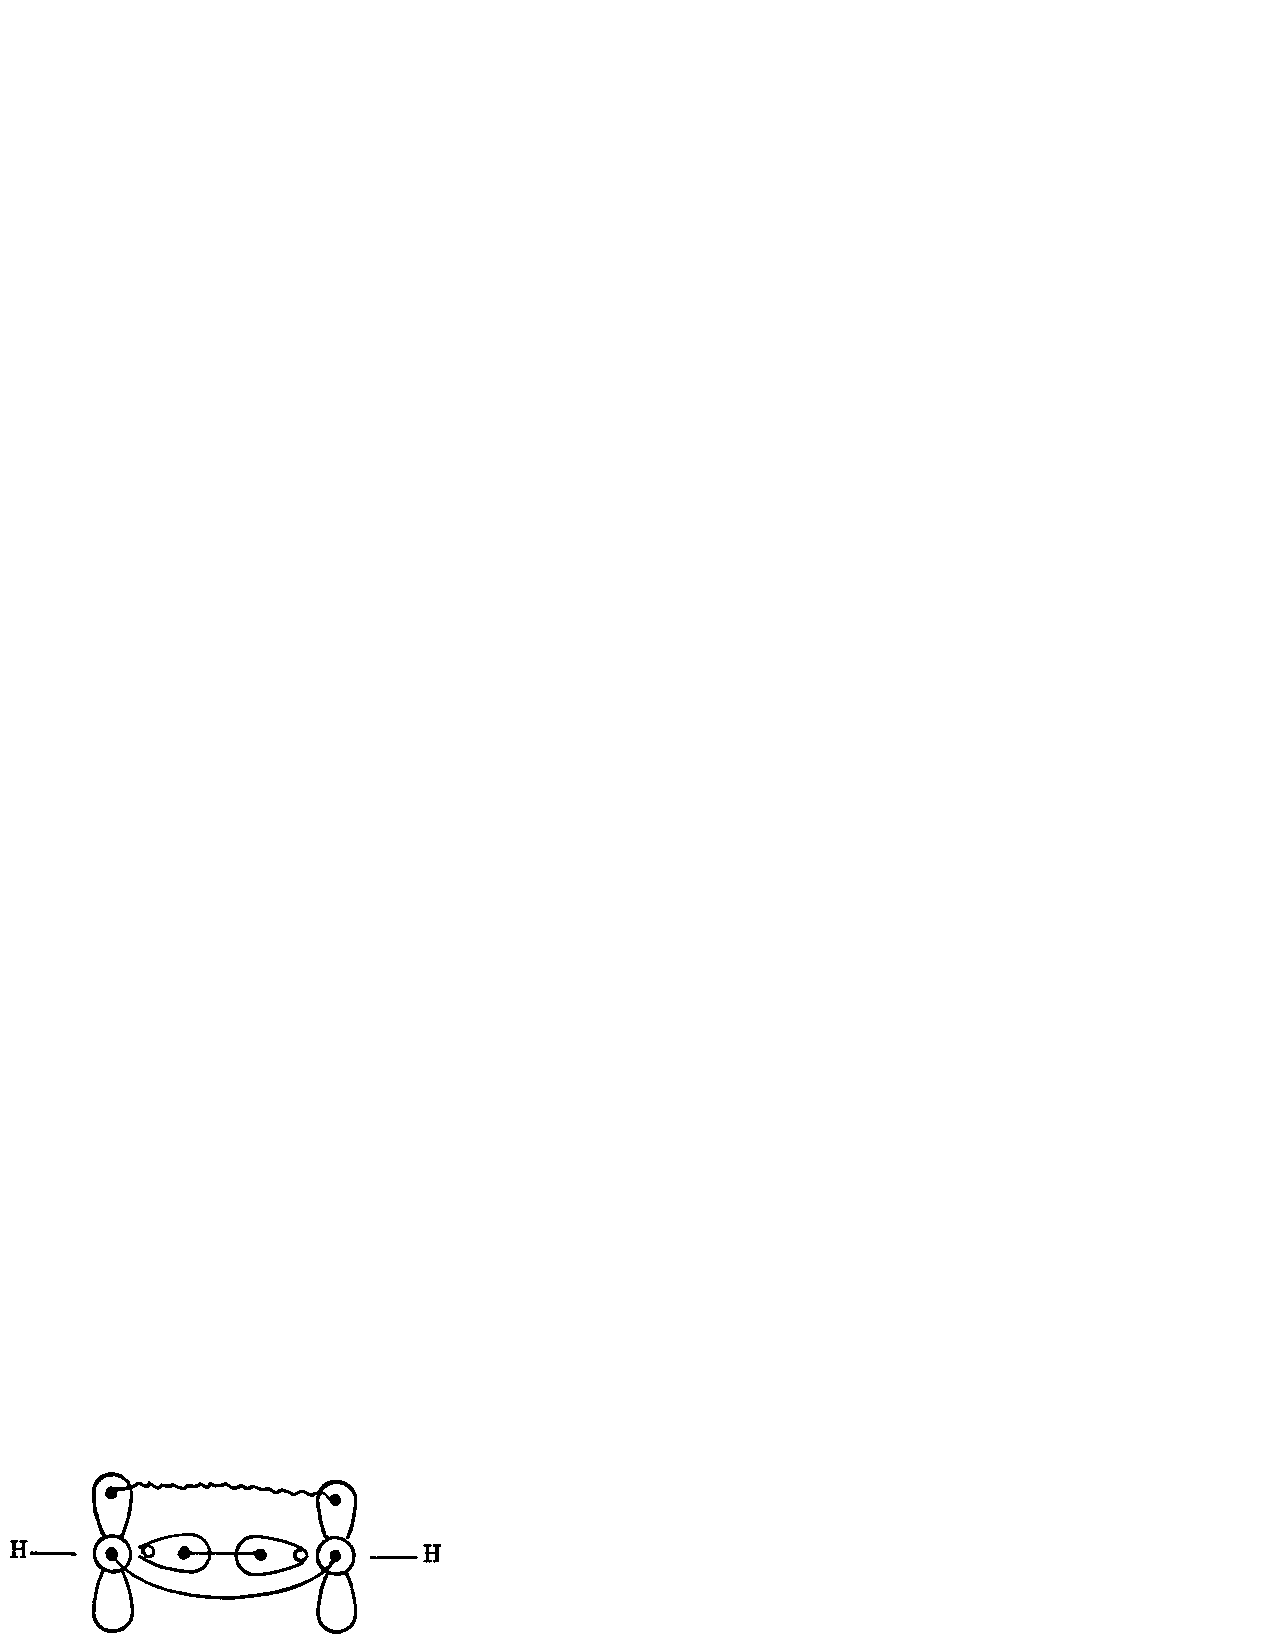
\includegraphics{fg7-9a}
\label{chap7-eqno35}
\end{equation}
where the two $\pi$ orbitals in the plane are triplet coupled.  Allowing 
distortions such as
\begin{equation}
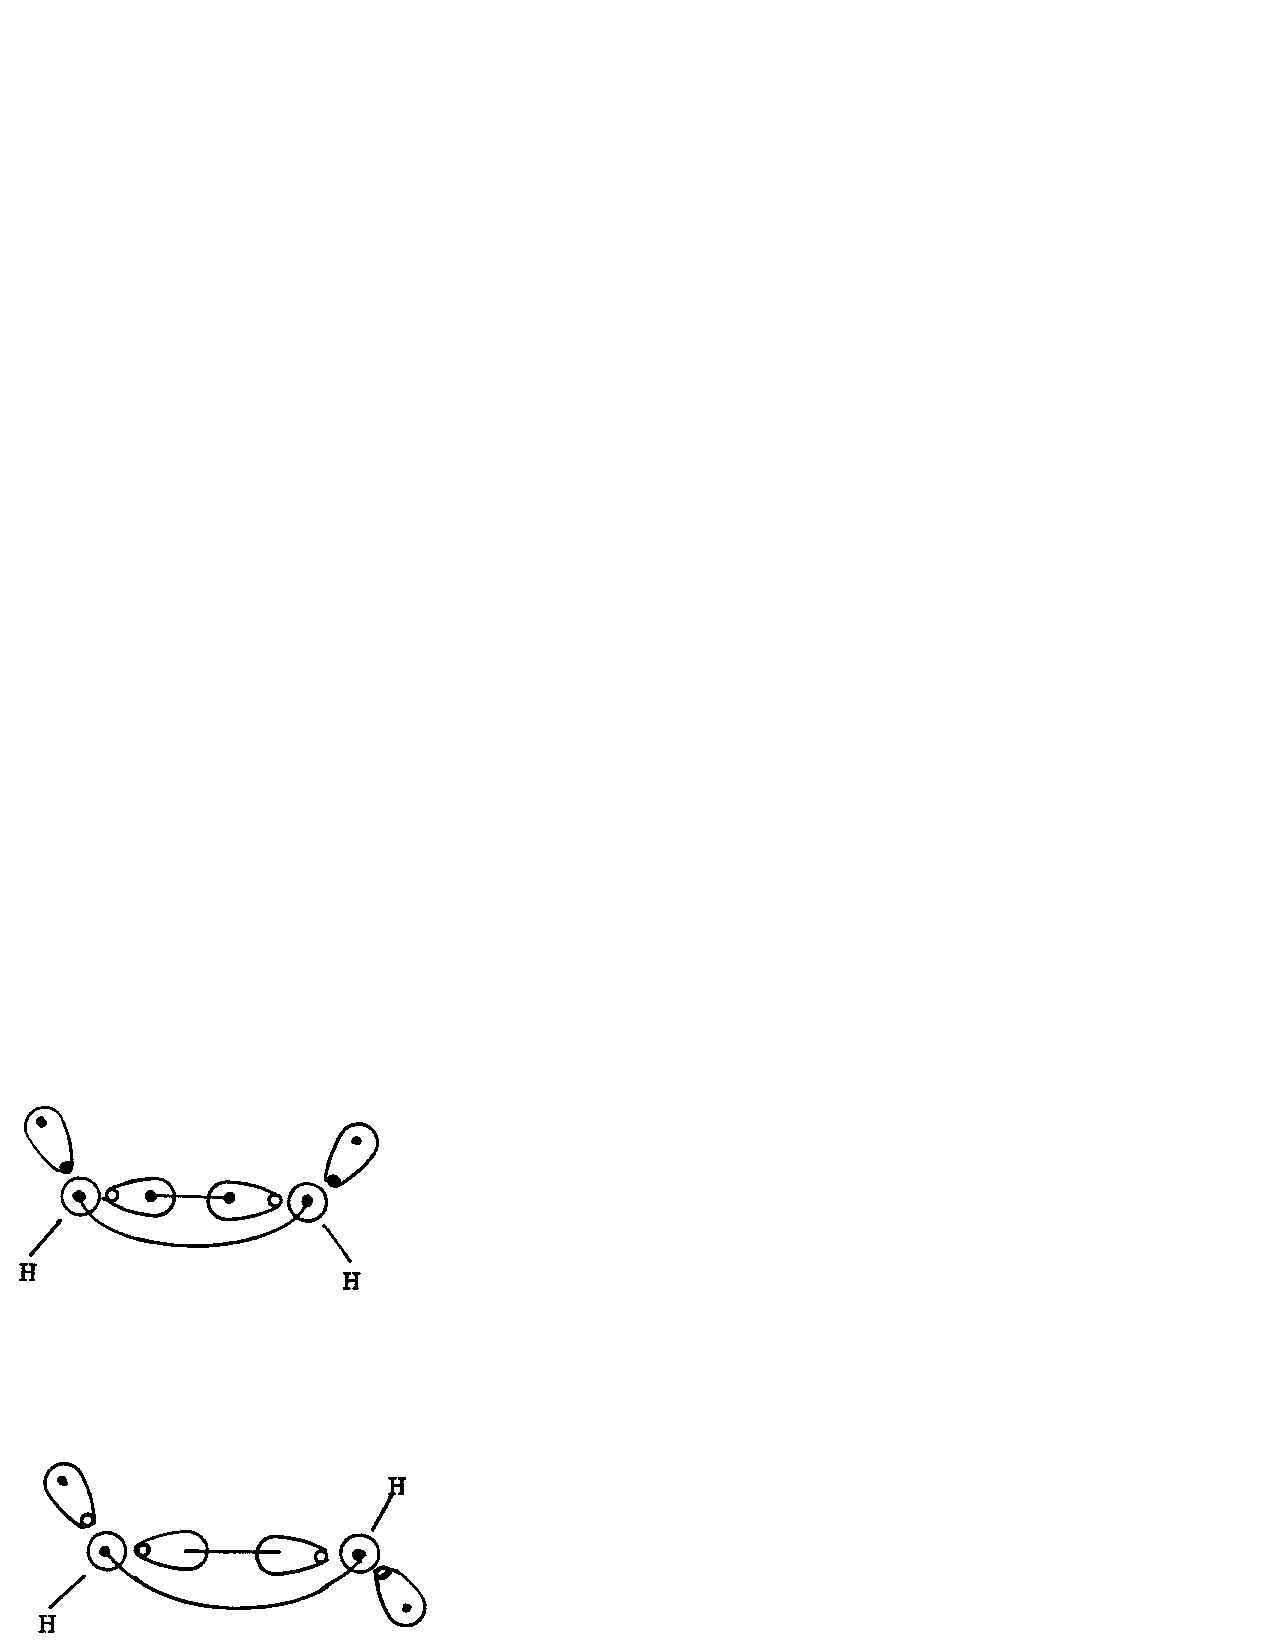
\includegraphics{fg7-9b}
\label{chap7-eqno37}
\end{equation}
decreases the $\pi_{\ell}\pi_r$ overlap, stabilizing the $\sigma$ triplet 
state.  Based on the geometry of triplet CH$_2$, 132$^{\circ}$, we would 
expect each HCC bond to be approximately 132$^{\circ}$ in order to optimize the 
orientation of the $\sigma$ bonds on each C.  Calculations predict 
the cis form is bent 128$^{\circ}$, and is more stable than the trans 
form, 131$^{\circ}$.

\subsection{Rotational Symmetry in Acetylene}

The $\pi$ bonds of acetylene (\ref{chap7-eqno30}) are drawn in two
orthogonal planes, e.g., $xz$ and $yz$.  However, the total
wavefunction is symmetric about the CC axis, i.e., a ${^1\Sigma}_g$
state. This can be seen by considering the wavefunction
\begin{equation}
A \left( \pi_x \alpha \right) \left( \pi_y \alpha \right)
\label{chap07-eqno38}
\end{equation}	
Rotating the wavefunction about the CC axis by an angle gamma 
leads to new orbitals
\begin{eqnarray}
{\bar{\pi}}_x &=& \pi_x \cos \gamma + \pi_y \sin \gamma\cr
{\bar{\pi}}_y &=& - \pi_x \sin \gamma + \pi_y \cos \gamma
\label{chap07-eqno39}
\end{eqnarray}
The resulting wavefunction is
\begin{eqnarray}
A \left[ \left( {\bar{\pi}}_x \alpha \right) \left( {\bar{\pi}}_y 
\alpha \right) \right] & = \cos^2 \gamma A \left[ \left( \pi_x \alpha 
\right) \left( \pi_y \alpha \right) \right] - \cos \gamma \sin \gamma 
A \left[ \left( \pi_x \alpha \right) \left( \pi_x \alpha \right) 
\right]\cr
& - \sin^2 \gamma \underbrace{A \left[ \left( \pi_y \alpha \right) \left( \pi_x 
\alpha \right) \right]}_{- A \left[ 
\left( \pi_x \alpha \right) \left( \pi_y \alpha \right) \right]}   
 + \sin \gamma \cos \gamma A \left[ \left( 
\pi_y \alpha \right) \left( \pi_y \alpha \right) \right]\cr
& = \left( \cos^2 \gamma + \sin^2 \gamma \right) A \left[ \left( 
\pi_x \alpha \right) \left( \pi_y \alpha \right) \right] = A \left[ 
\left( \pi_x \alpha \right) \left( \pi_y \alpha \right) 
\right].
\label{chap07-eqno40}
\end{eqnarray}
That is, the wavefunction (\ref{chap7-eqno38}) is left invariant,
unchanged, upon rotation about the CC axis.  Hence,
(\ref{chap7-eqno38}) is a $\sigma$ state.

Consequently, the wavefunction
\begin{equation}
A \left[ \left( \pi_x \alpha \right) \left( \pi_x \beta \right) 
\left( \pi_y \alpha \right) \left( \pi_y \beta \right) 
\right]
\label{chap07-eqno41}
\end{equation}
is also a $\Sigma$ state.  Considering spin, inversion, and vertical
reflection. we see that (\ref{chap7-eqno41}) is ${^1\Sigma}^+_g$.

\bigskip

\section{Bond Energies}

Next we will consider the energetics of CC bonds.  How strong are the
bonds?  First, however, we must consider what a bond energy is.
Consider a molecule $AB$ that dissociates into fragments $A$ and $B$,
each of which may be molecules, upon breaking the bond between two
atoms.  As indicated in Figure \ref{chap7-fig10}(a), the bond energy
$D(A - B)$ is just the energy difference
\begin{equation}
D_e (A-B) = E_e (A) + E_e (B) - E_e (A-B)
\label{chap07-eqno42}
\end{equation}
where the $E_e$ indicates that the fragments $A$ and $B$ have relaxed to 
their equilibrium configurations, and that $AB$ is in its equilibrium 
configuration.



\begin{figure}
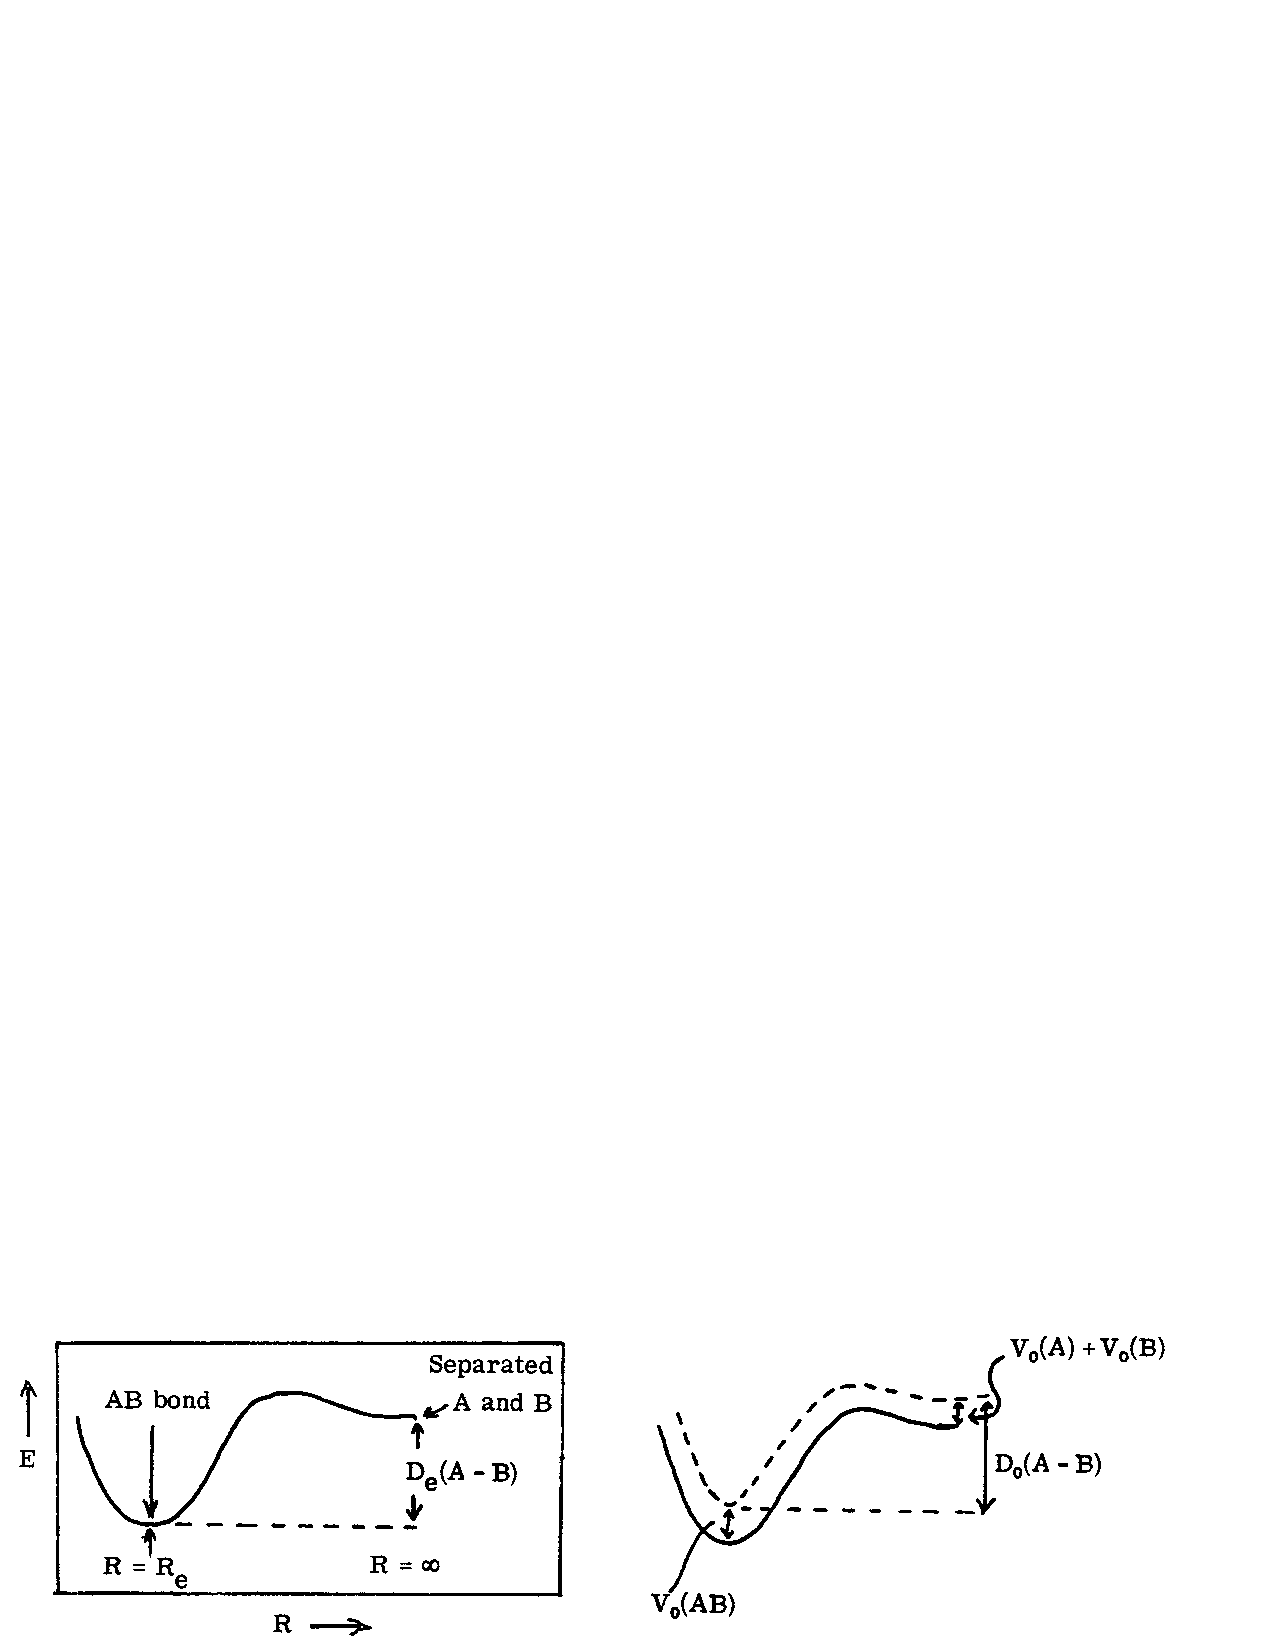
\includegraphics[scale=0.75]{fg7-10}
\caption{}
\label{chap7-fig10}
\end{figure}


The quantity (\ref{chap7-eqno42}) is obtained directly from
theoretical calculations of the energy as a function of geometry,
however, it cannot be measured directly.  The reason is that even at
$T = 0^{\circ}$K, there is zero-point energy in an the vibrational
modes of $A-B$, $A$, and $B$ so that the experiment measures
\begin{equation}
E_0 = E_e + V_0
\label{chap07-eqno43}
\end{equation}
where $V_0$ is the vibrational energy in the ground, $v = 0$, vibrational 
levels.  Thus, the experimental bond energy, at $T = 0^{\circ}$K, is
\begin{equation}
D_0 (A - B) = E_0 (A) + E_0 (B) - E_0 (AB)
\label{chap07-eqno44}
\end{equation}

\subsection{Temperature Corrections}

To make matters more complicated, the experiments are often carried 
out at finite temperature, to be specific we will assume 
$T = 298^{\circ}$K = 77$^{\circ}$F, somewhat less than summertime 
room temperature much more than the wintertime value, in these energy conscious 
times.  The experiments lead to energy changes at constant 
pressure and hence, the enthalpy $H = E + pV$ in the relevant 
quality. The bond energy at finite temperature is defined as
\begin{equation}
D_T(A - B) = H_T(A) + H_T(B) - H_T(A - B)
\label{chap07-eqno45}
\end{equation}
Thus, the relation between the bond energy at $T = 0^{\circ}$K, and that 
at 298$^{\circ}$K is
\begin{eqnarray}
D_{298^{\circ}{\rm K}} - D_{0^{\circ}{\rm K}} & =& \sum^{T}_{0} \left[ C_p (A) + 
C_p (B) - C+p (AB) \right] dt\cr
& \approx & 0.9 ~ {\rm kcal/mol ~ if} ~ A ~ {\rm and} ~ B ~ {\rm are ~ atoms}\cr
& \approx & 1.5 ~ {\rm kcal/mol ~ if} ~ A ~ {\rm is ~ an ~ atom, ~ and} ~ 
B ~ {\rm is ~ nonlinear}\cr
& \approx& 2.4 ~ {\rm kcal/mol ~ if} ~ A ~ {\rm and} ~ B ~ {\rm are ~ 
nonlinear}.
\end{eqnarray}

Only the translational and rotational contributions are included 
here.   This assumes that all vibrational energies are much greater 
than $RT = 0.6$ kcal = 210 cm$^{-1}$.  Thus, $C_p$ in kcal/mol is ${5 
\over 2}R$ for atoms, ${7 \over 2}R$ for linear 
molecules and $4R$ for nonlinear molecules.

A slight additional complication is that the experimental data 
are not tabulated as absolute enthalpies.  Rather the enthalpy, 
say of C$_2$H$_6$, is referenced to that of the free elements carbon 
and hydrogen each in their ground states, graphite for carbon 
and H$_2$ for hydrogen. This, relative enthalpy, is referred to as the 
heat of formation and denoted as $\Delta H^0_{fT}$.  Thus, 
$\Delta H^0_{f,298^{\circ}{\rm K}}$ (C$_2$H$_6$) = $-$20.24 kcal/mol 
means that 20.24 kcal of energy is liberated upon forming one 
mole of ethane, at atmospheric pressure and 298$^{\circ}$K, from appropriate 
amounts of hydrogen gas and graphite, at atmospheric pressure and 
298$^{\circ}$K.  Since 
\begin{equation}
\Delta H^0_{f,298^{\circ}{\rm K}} (\chem{CH_3}) = 34.82~\mathrm{kcal/mol}, 
\end{equation}
we see that
\begin{equation}
D_{298^{\circ}{\rm K}} (\chem{H_3C-CH_3}) = 2 \times 34.82 + 
20.24 = 89.88 ~ {\rm kcal/mol}
\label{chap07-eqno47}
\end{equation}
Using (\ref{chap7-eqno46}), we obtain
\begin{equation}
D_{0^{\circ}{\rm K}} (\chem{H_3C-CH_3}) = 89.9 - 2.4 = 87.5 
~ {\rm kcal/mol}
\label{chap07-eqno48}
\end{equation}
When making comparisons to theory or to spectroscopic 
experiments, the bond energy at 0$^{\circ}$K is more convenient. 
However, in discussing chemical reactions, the bond energy at 
298$^{\circ}$K is generally most convenient. In this course it will be 
understood that bond energies are at 298$^{\circ}$K unless stated otherwise.

\medskip

\subsection{Ethane}

\begin{table}
\caption{ Geometry and zero point energy, $V_0$.  
$V_0$ is based on the harmonic approximation and is probably not 
accurate to more than 0.1 kcal/mol.  All values in square brackets 
are based on crude estimates.}
\label{chap7-tab1a}
\begin{tabular}{ccccc}\\ \hline
&\multicolumn{3}{c}{Geometry}&$V_0$\cr
& CC & CH & HCH\cr
& (\AA) & (\AA) & & (kcal)\cr

HC $\equiv$ CH & 1.208 & 1.056 & & 16.18\cr
H$_2$CH-CH$_2$ & 1,339 & 1.086 & 117.6$^{\circ}$ & 30.89\cr
H$_2$CCH$_2$ & 1.50 & & 117.6$^{\circ}$ & [28.6]\cr
H$_3$C$-$CH$_3$ & 1.526 & 1.095 & 107.7$^{\circ}$ & 43.90\cr
CH$_2$(${^3\Pi}$) & - & 1199$^c$ & - & 4.09\cr
CH$_2$(${^3B}_1$) & - & 1.084$^a$ & 133.2$^a$ & 10.4$^a$\cr
CH$_3$ & - & 1.079$^e$ & 120 & 18.18\cr
CH$_4$ & - & 1.091$^e$ & 109.46$^{\circ}$ & 27.10\cr
\hline
\end{tabular}
\end{table}

\begin{table}
\caption{Average vibrational frequencies, cm$^{-1}$.}
\label{chap7-tab1b}
\begin{tabular}{cccccc}\\ \hline
& CC & CH & HCH & CH$_n$ & Other\cr
& & Scissors & Rock\cr

HC $\equiv$ CH & 1974$^b$ & 3332(2) & - & 671(4)\cr
H$_2$CH$-$CH$_2$ & 1623$^b$ & 3056(4) & 1393(2) & 995(5)\cr
H$_2$CCH$_2$ & [995] & 3056(4) & 1393(2) & [995](4)\cr
H$_3$C$-$CH$_3$ & 995$^b$ & 2960(6) & 1440(6) & 1006(4) & Torsion 
289\cr
CH$_2$(${^3\Pi}$) & - & 2859$^c$ & - & -\cr
CH$_2$(${^3B}_1$) & - & 3080(2)$^d$ & 1114\cr
CH$_3$ & - & 3123(3)$^d$ & 1383(2) & - & Inversion 580\cr
CH$_4$ & - & 2994(4)$^b$ & 1397(5) & -\cr
\hline
\end{tabular}\\
$^a$ L. B. Harding and W. A. Goddard III, CPL, volume 55, 217 (1978).
$^b$ NSRDS-NBS 92, T. Shimanouchi, Tables of Molecules Vibrational 
Frequencies.
$^c$ G. Herzberg and K. Huber, Diatomic Molecules.
$^d$ JANAF Tables.
$^e$ G. Herzberg, Electronic Spectra of Polyatomic Molecules.
$^f$ $V_0$ is based on the harmonic approximation and is probably
not accurate to more than 0.1 kcal/mol.
\end{table}


As an example, consider ethane.  The bond energy at 0$^{\circ}$K is
$D_{0^{\circ}{\rm K}} =$ 87.5 kcal/mol.  In order to obtain $D_e$, we
must obtain zero point energies of ethane and methyl. The vibrational
frequencies of these molecules are listed in Table
\ref{chap7-table1a}--\ref{chap7-table1b}.  For a harmonic oscillator
of frequency $\nu$ (Hz) the zero point energy is $V_0 = {1 \over 2} h
\nu = {1 \over 2} \hbar \omega$.  Thus, an approximate estimate of the
zero point energy is
\begin{equation}
V_0 = {1 \over 2} \sum_{i} \left( h \nu_i \right).
\end{equation}
as indicated in Table \ref{chap7-tab1a}--\ref{chap7-tab1b}, this leads
to $V_0$(CH$_3$) = 18.2 kcal, and $V_0$(C$_2$H$_6$) = 43.9 kcal, and
hence, $D_e = D_0 + 7.5$ kcal/mol = 95.0 kcal/mol.

In breaking the CC bond of ethane, the geometry changes from
CC = 1.526 \AA, HCH = 107.7$^{\circ}$, CH = 1.095 \AA\
to CC = $\infty$, HCH = 120$^{\circ}$, CH = 1.079 \AA.  Thus,
the actual bond energy includes not only a quantity intrinsic to 
ethane but also a relaxation ion energy associated with the 
fragment.  A useful way to think about this is to separate the bond 
breaking process into two steps. First, the bond snap.  Here we consider 
stretching the CC bond of ethane to infinity while keeping all other 
bonds fixed, e.g., HCH = 107.7$^{\circ}$ and CH = 1.095\AA.  Then, 
secondly, the fragment relaxation.  Here we obtain the CH$_3$ fragments 
to relax to their equilibrium geometry, HCH = 120$^{\circ}$ and CH = 
1.097 \AA.

The relaxation energy for CH$_3$ is 7.3 kcal, so that the bond snap 
energy of ethane is
\begin{equation}
D^{snap}_e (\chem{H_3C-CH_3}) = 95.0 + 14.6 = 109.6 {\rm kcal}.
\end{equation}
This bond snap energy is intrinsic to the electronic structure of the 
bonded molecule.  Hence, comparisons of bond snap energies of various 
molecules might exhibit a regular behavior that could be interpreted 
in terms of interactions within the molecule, as distinct from 
differential effects in relaxation of the fragments.

\subsection{Effects of Ligands upon CC Bond Energies}

\begin{table}
\caption{CC single bond energies, kcal/mole at 298$^{\circ}$K.  Values
in parentheses are the $\Delta H_f$ for the radicals, 298$^{\circ}$K.}
\label{chap7-tab2}
\begin{tabular}{ccccc}\\ \hline

& CH$_3$ & CH$_2$Me & CHMe$_2$ & CMe$_3$\cr

CH$_3$ (+34.84) & 89.9 & 85.7 & 85 & 82.5\cr
CH$_2$Me (+26) & & 82 & 81\cr
CHMe$_2$ (+18) & & & 78.5 & 75\cr
CMe$_3$ (+8) & & & & 70\cr
\hline
\end{tabular}
\end{table}

First consider single bonds.  In Table \ref{chap7-tab2}, we show the
strengths of a CC single bond for various cases.  The values vary from
$D(\chem{H_3C-CH_3}) = 89.9$ kcal to $D(\chem{Me_3C-CMe_3}) = 70$
kcal.  There are three plausible explanations for these variations,
they are:
\begin{enumerate}
\item Inductive effects.  A change in the character of 
the C-C bond orbital due to replacement of an H ligand by the Me;
\item	Fragment relaxation effects.  Because of the larger size 
of Me as compared to H, there will be larger ligand-ligand interactions 
and hence, a bigger relaxation energy in the fragment upon relaxing 
from tetrahedral to planar geometries. amd
\item Ligand-CC pair-pair repulsion.  Each H to Me substitution 
leads to two additional CH bonds that are gauche to the original CC 
bond. These additional CH interactions weaken this CC bond.  For 
example, in C$_2$H$_6$ there are six interactions between gauche 
CH pairs on opposite carbons, as indicated in (\ref{chap7-eqno49}(b)).
Breaking the CC bond eliminates these six bad interactions.
With an Me substituent, there are additional repulsive interactions.
\begin{equation}
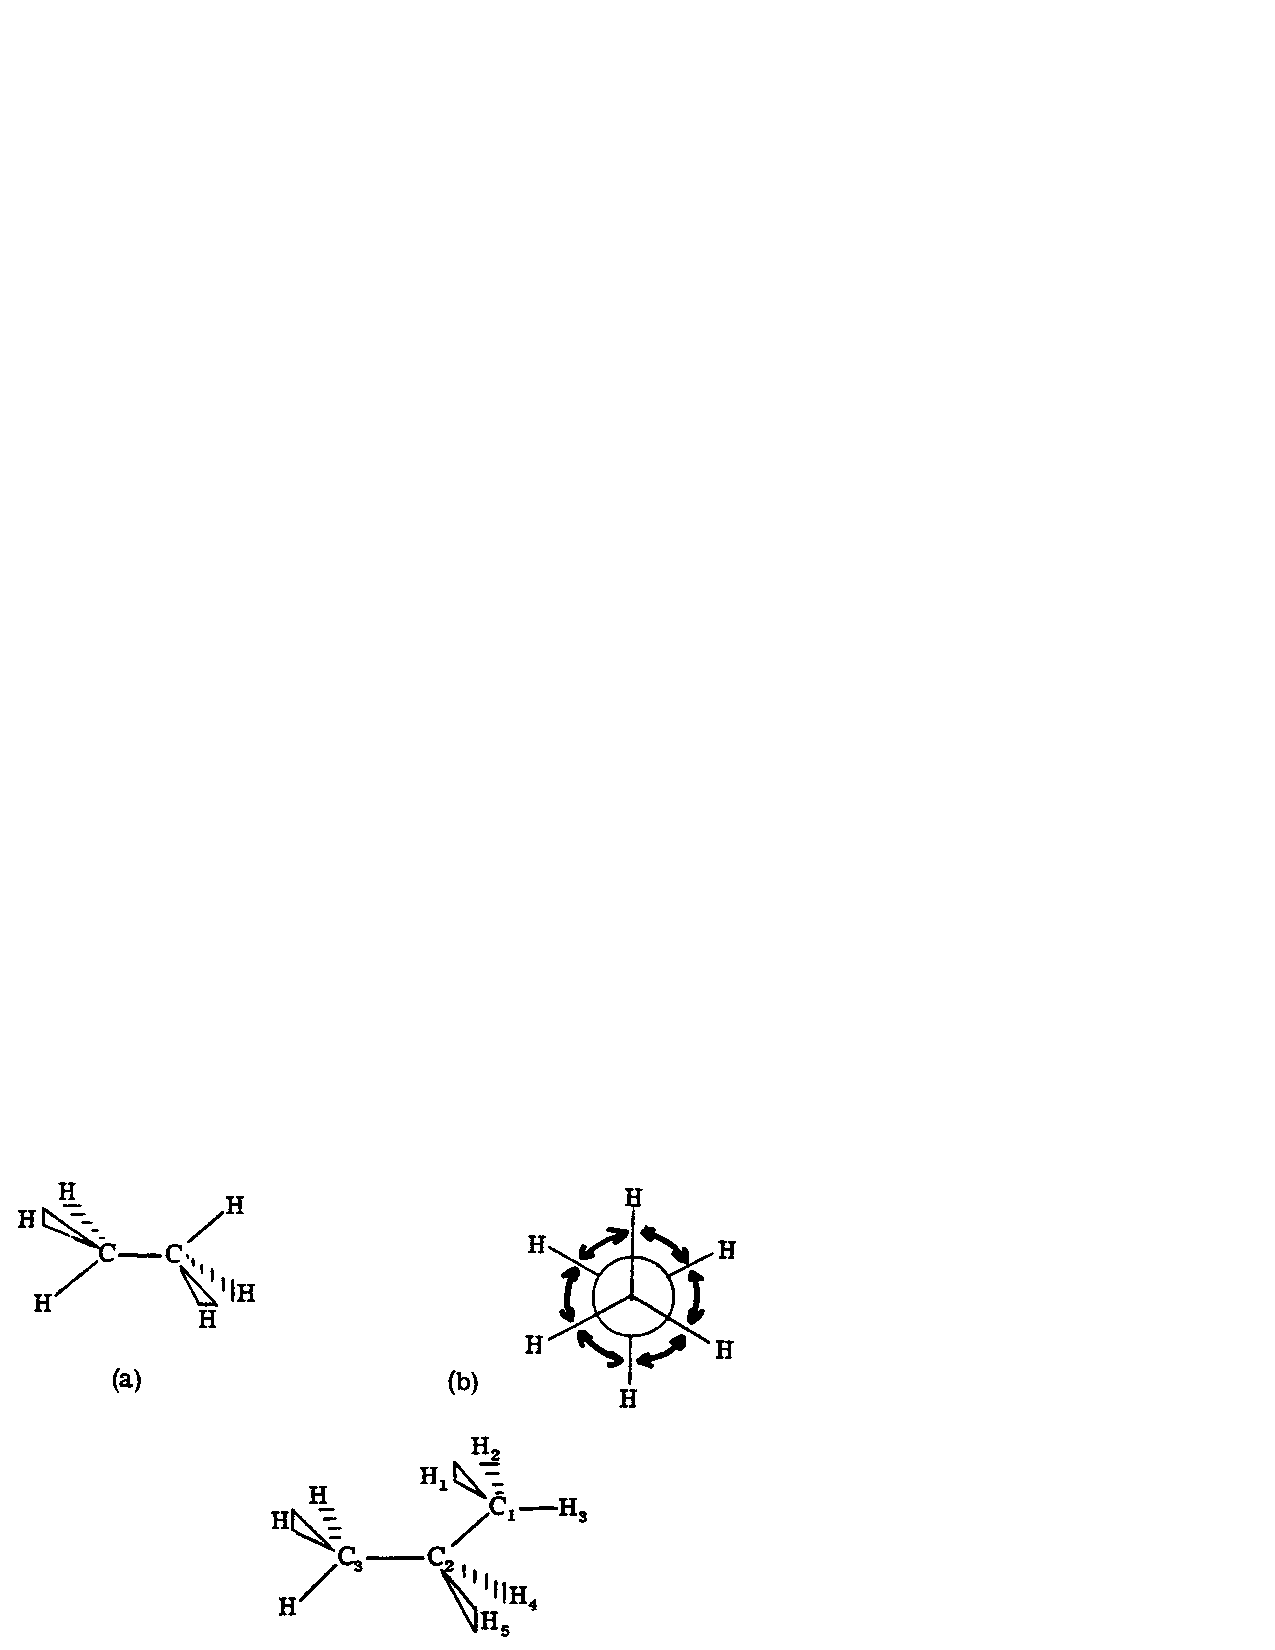
\includegraphics{fg7-10a}
\label{chap7-eqno49}
\end{equation}
The C$_2$C$_3-$C$_1$H$_1$ and C$_2$C$_3-$C$_2$H$_2$ interactions are
removed as the C$_2$C$_3$ bond is broken, thereby leading to a
decreased bond energy.  Including such effects, one would expect
linear changes in each horizontal and vertical step of Table
\ref{chap7-tab2}, a result that is approximately true.
\end{enumerate}
It is not known which of the effects (i) to (iii) dominate.

\begin{table}
\caption{Bond energies for CC double bonds, kcal/mole at 298$^{\circ}$K.}
\label{chap7-tab3}
\begin{tabular}{cccc}\\ \hline

& CH$_2$ & CHMe & CMe$_2$\cr

CH$_2$ (92.4) & 172.3 & 168.5 & 167.4\cr
CHMe (81) & & 164 & 162\cr
CMe$_2$ (71) & & & 1.59\cr

\hline
\end{tabular}
\end{table}

\begin{table}
\caption{Comparison of energy quantities for substituted alkenes.}
\label{chap7-tab4}
\begin{tabular}{ccccccccc}\\ \hline

&&& &\multicolumn{3}{c}{Ground State}&$N$ to $T$ & $N$ to $V$\cr
&&& & Bond Energy & Bond Length & Rotation Barrier &
\multicolumn{2}{c}{Separation}\cr
&&& & (kcal/mol) & (\AA) & (kcal/mol) & (eV) & (eV)\cr

&&& & 172.3 & 1.339 & 65 & 4.32 & 7.6\cr

&&& & 168.5 & 1.336 & & 4.28 & 7.17\cr

&&& & 163 & & 63-65 & 4.21 & 7.10\cr

&&& && 164 & & 4.24 & 6.95\cr

&&& && 167.4 & & 4.22 & 6.6-6.7\cr

&&& && 162 & & 4.16 & 6.8-7.0\cr

&&& && 159 & & 4.10 & 6.57\cr
\hline
\end{tabular}
\end{table}

Now let us consider multiple bonds.  Substituting the H's of ethylene
with various saturated groups leads to alkenes with an electron
structure qualitatively similar to ethylene.  In general, the bonding
and antibonding orbitals are denoted as $\pi$ and $\pi*$,
respectively, rather than $\pi_u$ and $\pi_g$, but the notation $N$,
$T$, and $V$ is still used.  The trend in bond energies for various
simple alkenes, is given in Table \ref{chap7-tab3}, while other
properties are tabulated in Table \ref{chap7-tab4}.

\begin{table}
\caption{Bond energies for CC triplet bonds, kcal/mol at 298$^{\circ}$K.}
\label{chap7-tab5}
\begin{tabular}{ccc}\\ \hline

& CH & CMe\cr

CH (142.0) & 229.8 & 228\cr
CMe (130) & & 225\cr
\hline
\end{tabular}
\end{table}

\begin{table}
\caption{CC bond energies, kcal/mole.  This is based on the simple
correation, and ignores vibrational contributions to
$D_{298^{\circ}{\rm K}} = D_{0^{\circ}{\rm K}}$.}
\label{chap7-tab6}
\begin{tabular}{ccccccc}\\ \hline

&\multicolumn{4}{c}{CC Bond Energy}&\multicolumn{2}{c}{Incremental $D_e$}\cr
&\multicolumn{3}{c}{Adiabatic}&Snap&Adiabatic&Snap\cr
&$D_{298{\rm K}}$ & $D_{0{\rm K}}$ & $D_e$$^a$ & $D_e$\cr
\noalign{\medskip\hrule\medskip}
H$_3$C$-$CH$_3$ & 89.9 & 87.5 & 95.0 & 109.6$^b$ & 95 & 110\cr
H$_2$C=CH$_2$ & 172.3 & 169.9 & 180.0 & 184.7$^c$ & 85 & 75\cr
H$_2$C$-$CH$_2$$^f$ & [107.3]$^d$ & [105.2] & [113.0] & [117.7]\cr
HC$\equiv$CH & 229.8 & 227.7 & 235.7 & 269.7$^e$ & 56 & 85\cr
\hline
\end{tabular}\\
$^a$Using $V_0$ from Table 7-1.
$^b$Using 7.3 kcal for the relaxation energy of CH$_3$.
$^c$Using 4.7 kcal for the relaxation energy of CH$_2$.
$^d$Assuming a rotational barrier of 65 kcal for ethylene at 
298$^{\circ}$K. 
$^e$Using 17 kcal for the electronic excitation energy from 
${^2\Pi}$ to ${^4\Sigma}^-$.
$^f$Twisted.
\end{table}

Substituting the H's of acetylene with various saturated groups leads to
other alkynes, whose trends in bond energy are given in Table 
\ref{chap7-tab5}.

Secondly, let us consider comparison of CC bonds.  From Table
\ref{chap7-tab6} the adiabatic $D_e$ for C-C, C=C, and C$\equiv$C
bonds are 95, 180, and 236 kcal, respectively.  Thus, the $\pi$ bond of
ethylene is 85 kcal stronger than the $\sigma$ bond of ethane, and the
second $\pi$ bond of acetylene leads to an increase of 56 kcal in bond
energy over that of ethylene.

From the wavefunctions, there is no obvious reason why the two $\pi$ 
bonds of acetylene are proportionally weaker than the $\pi$ bond of 
ethylene.  Indeed, considering that ethylene has eclipsed CH bonds 
we might believe that the $\pi$ bond in ethylene would be weaker.  These 
views are strengthened by a comparison of the bond snap energies which 
are 110 kcal for C-C, 185 kcal for C=C, and 270 kcal for 
C$\equiv$C. In terms of bond snap energies the $\pi$ bond of ethylene 
is 75 kcal, while the total $\pi$ bonding of acetylene is 160 kcal or 
80 kcal apiece.  The reason why the adiabatic bond energy is so weak, 
is that each CH fragment must be promoted, at a cost of 17 kcal each, 
to the ${^4\Sigma}^-$ state
\begin{equation}
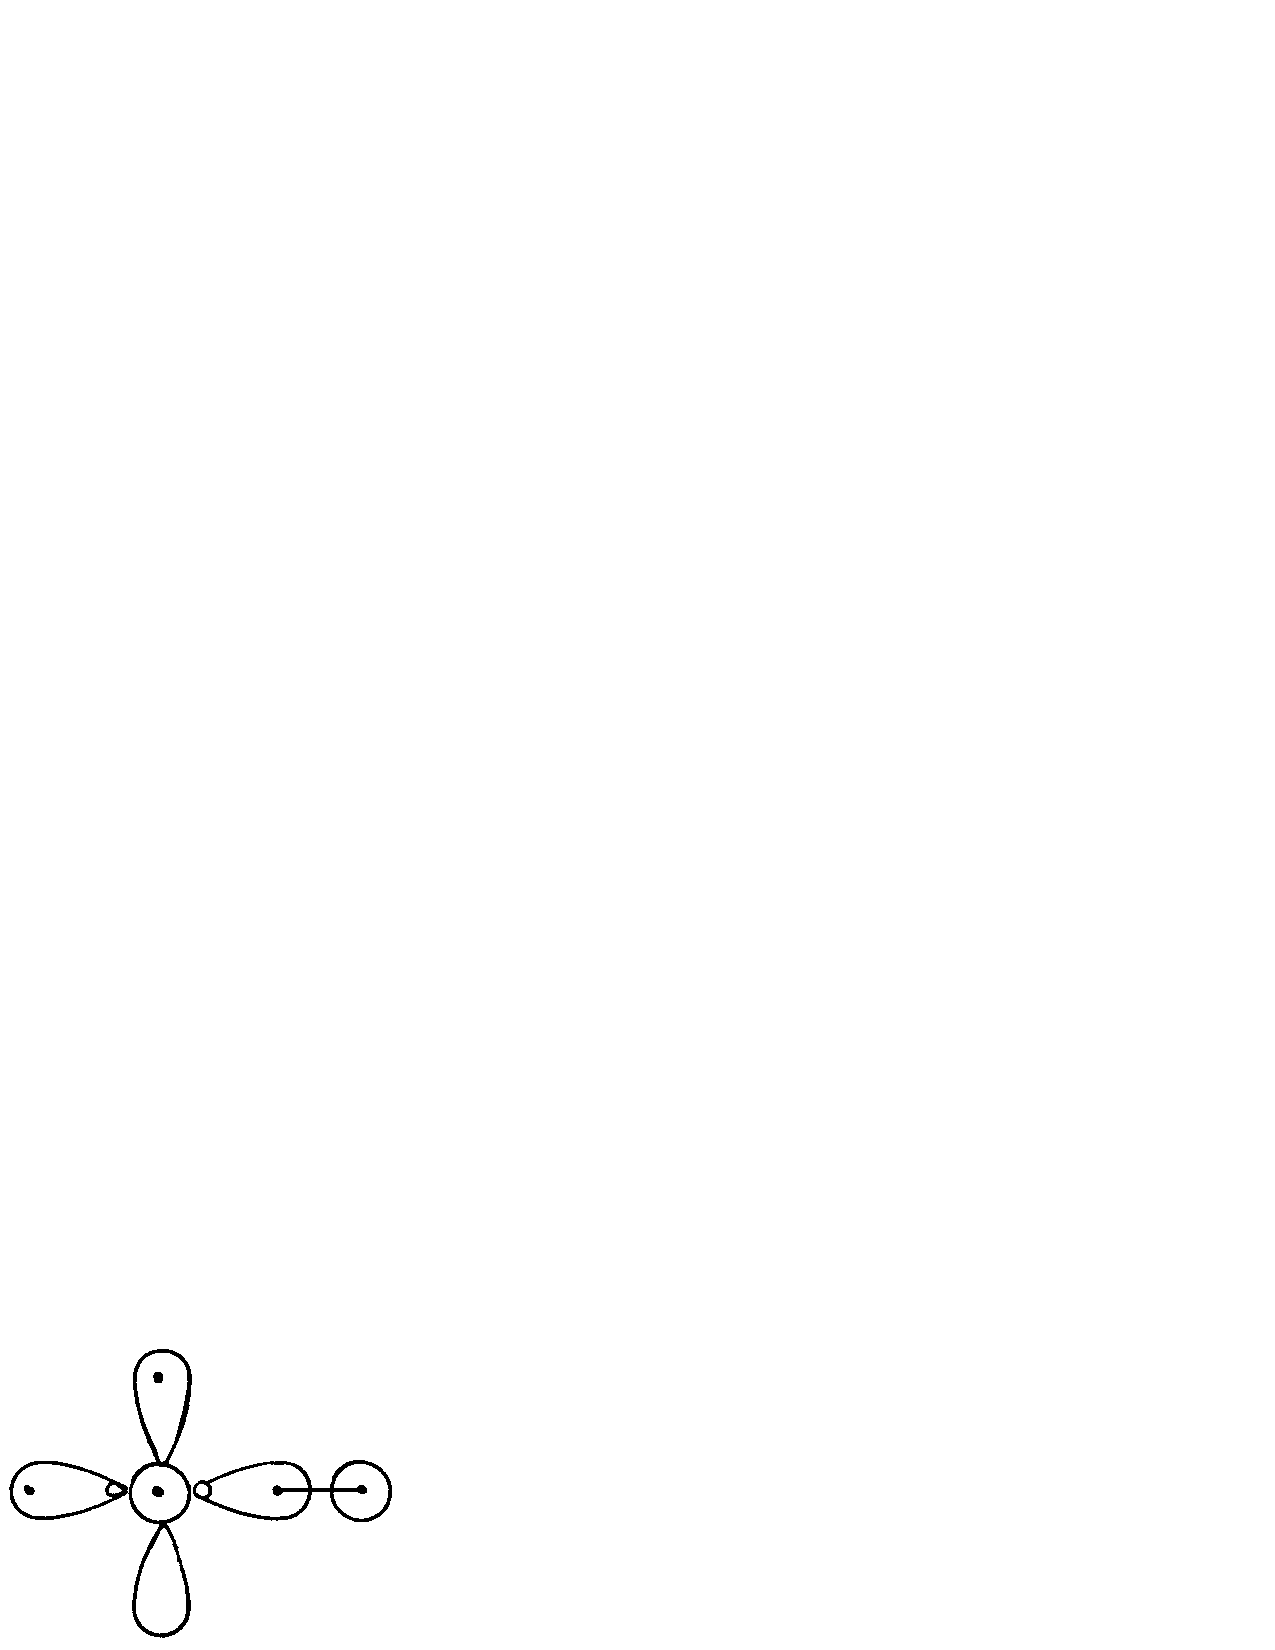
\includegraphics{fg7-10b}
\end{equation}
in order to make two $\pi$ bonds.  Perhaps the reason why the $\pi$ bond 
snap energy of ethylene is 5 kcal weaker than the average $\pi$ bond 
snap in acetylene, is the eclipsing of the CH bonds.

Experimentally the activation energy for cis-trans isomerization 
in ethylene is 65 kcal.  Since the CC bond energy of ethylene is 172 
kcal, this indicates that the CC bond energy of
\begin{equation}
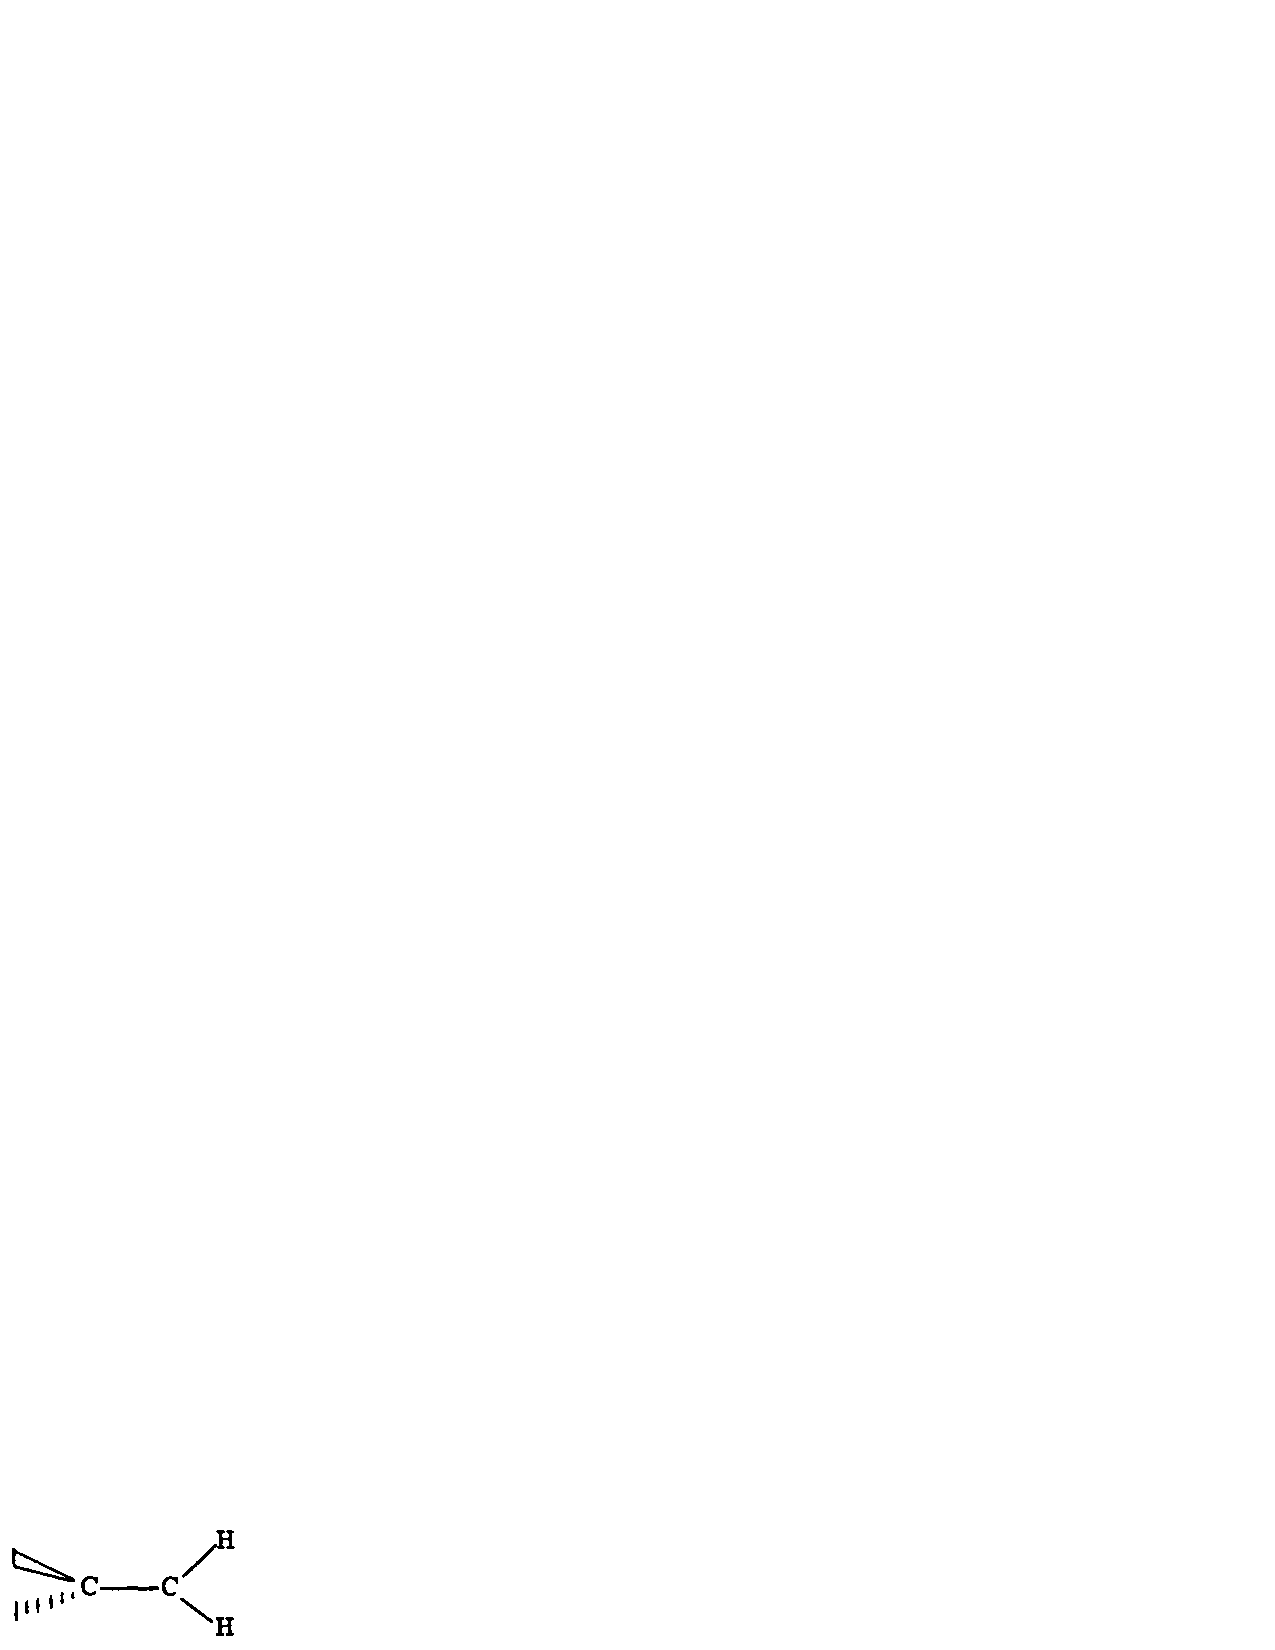
\includegraphics{fg7-10c}
\label{chap7-eqno51}
\end{equation}
is $D_{298} =$ 107 kcal, leading to a bond snap energy of 118 kcal. The 
difference between this value and the 110 kcal bond snap of ethane, 
I interpret as mainly due to the reduction of the pair-pair repulsions 
for CH bonds on opposing carbons, in ethane.

The CC bond distance for twisted ethylene is 1.50 \AA.  Assuming the 
C-H repulsions are negligible in twisted ethylene, this could be 
considered as the intrinsic length for a CC $\sigma$ bond with the 
additional 0.03 \AA\ in ethane due to nonbonded repulsion of the 
CH bonds.

Some other properties of these systems are tabulated in Table
\ref{chap7-tab6}. Note that the CC vibrational frequency increases
from 995, to 1623, to 1974 cm$^{-1}$ for single, double and triple
bonds.  There are also systematic changes in the CH vibrational
frequencies, cm$^{-1}$: 2960 for H$_3$CCH$_3$, and 2994 for CH$_4$;
3056 for H$_2$C=CH$_2$, 3080 for CH$_2$, and 3123 for CH$_3$; and,
3332 for HC$\equiv$CH.

\section{Resonance}

\subsection{Benzene}

Methyl radical is planar with 120$^{\circ}$ bond angles, and 
ethylene is planar with similar bond angles.  Thus, it is plausible 
that a cyclic C$_6$H$_6$ molecule would be planar with 120$^{\circ}$ 
bond angles
\begin{equation}
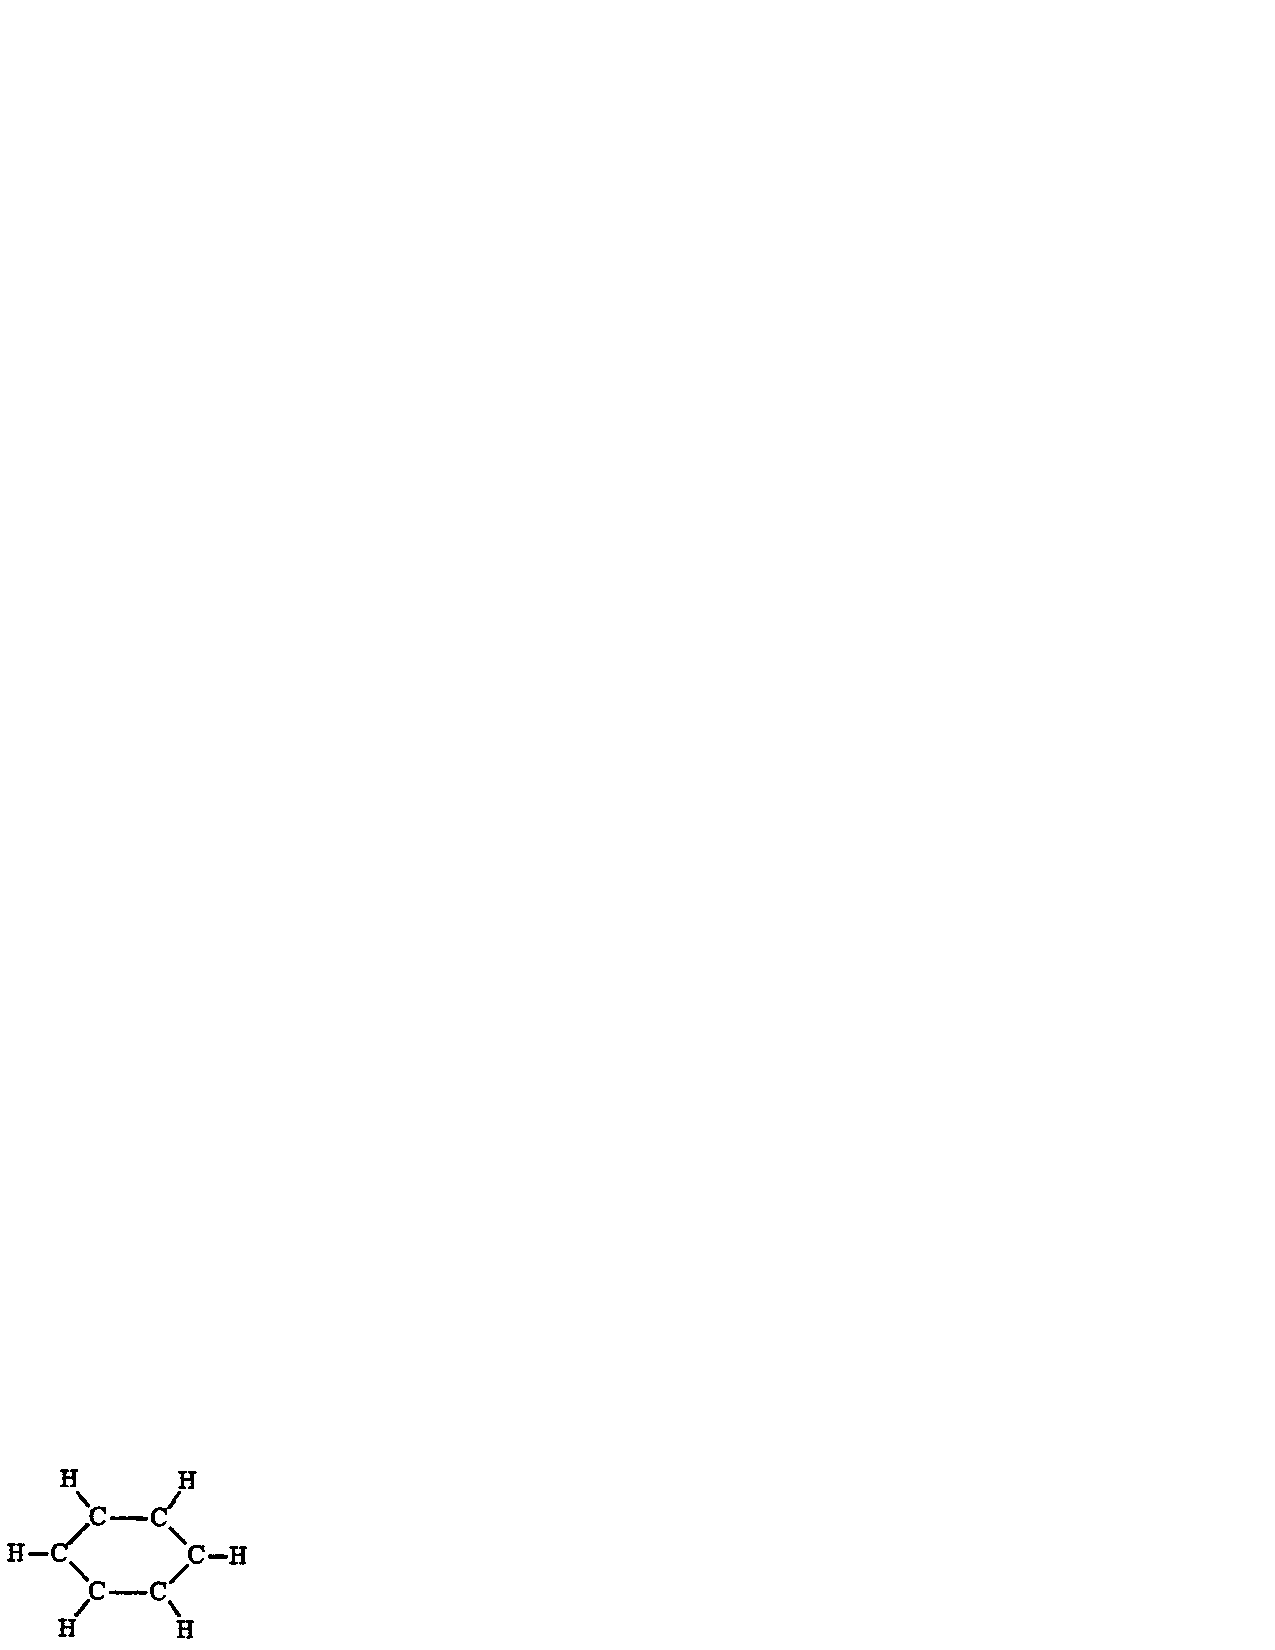
\includegraphics{fg7-10d}
\label{chap7-eqno52}
\end{equation}
The question is how to pair the six $\pi$ orbitals of
(\ref{chap7-eqno52}).  There are two obvious cases, known as the
kekule structures
\begin{equation}
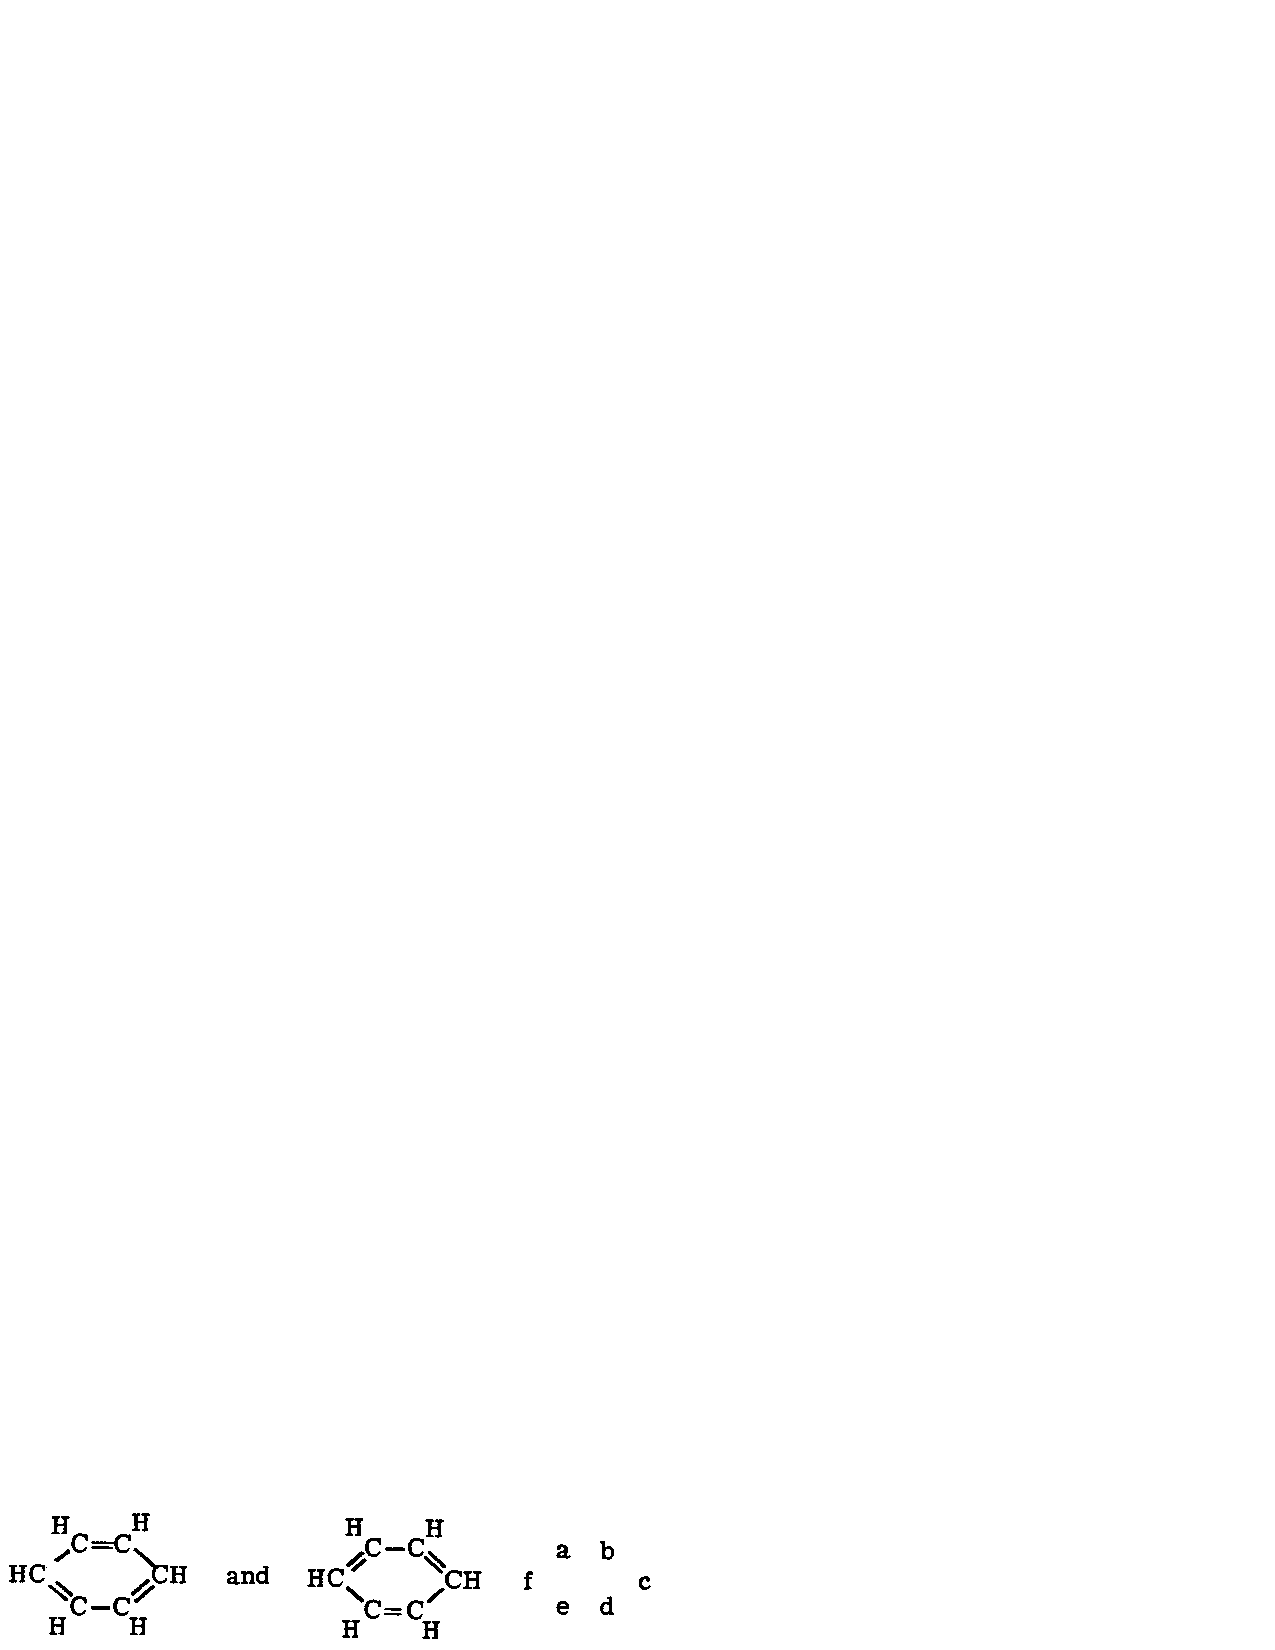
\includegraphics{fg7-10e}
\label{chap7-eqno53}
\end{equation}
with corresponding wavefunctions ($\pi$ system only)
\begin{eqnarray}
\psi_{2a} &=& A \left[ \left( \phi_a \phi_b + \phi_b \phi_a \right) 
\left( \phi_c \phi_d + \phi_d \phi_c \right) \left( \phi_e \phi_f + 
\phi_f \phi_e \right) \alpha \beta \alpha \beta \alpha \beta 
\right]\cr
&=& A \left[ \phi_a \phi_b \phi_c \phi_d \phi_e \phi_f \chi_{2a} 
\right]
\end{eqnarray}
where
\begin{equation}
\chi_{2a} = \left( \alpha \beta - \beta \alpha \right) \left( \alpha 
\beta - \beta \alpha \right) \left( \alpha \beta - \beta \alpha \right)
\end{equation}
and
\begin{eqnarray}
\psi_{2b} &=& A \left[ \left( \phi_b \phi_c + \phi_c \phi_b \right) 
\left( \phi_d \phi_e + \phi_e \phi_d \right) \left( \phi_f \phi_a + 
\phi_a \phi_f \right) \alpha \beta \alpha \beta \alpha \beta \right]\cr
&=& A \left[ \phi_b \phi_c \phi_d \phi_e \phi_f \phi_a  \left( \alpha 
\beta - \beta \alpha \right) \left( \alpha \beta - \beta \alpha 
\right) \left( \alpha \beta - \beta \alpha \right) \right]\cr
&=& A \left[ \phi_a \phi_b \phi_c \phi_d \phi_e \phi_f \chi_{2b} 
\right]
\end{eqnarray}
where
\begin{equation}
\chi_{2b} = \beta \left( \alpha \beta - \beta \alpha \right) \left( 
\alpha \beta - \beta \alpha \right) \alpha - \alpha \left( \alpha 
\beta - \beta \alpha \right) \left( \alpha \beta - \beta \alpha 
\right) \beta.
\end{equation}
Superimposing these wavefunctions leads to a new wavefunction
\begin{equation}
\chi_3 = A \left[ \phi_a \phi_b \phi_c \phi_d \phi_e \phi_f \chi_3 
\right]
\end{equation}
where $\chi_e = \chi_{2a} + \chi_{2b}$,
which corresponds to a superposition of the bonding structures 
in (\ref{chap7-eqno53}).  In $\chi_3$, all six bonds are equivalent, and we write
\begin{equation}
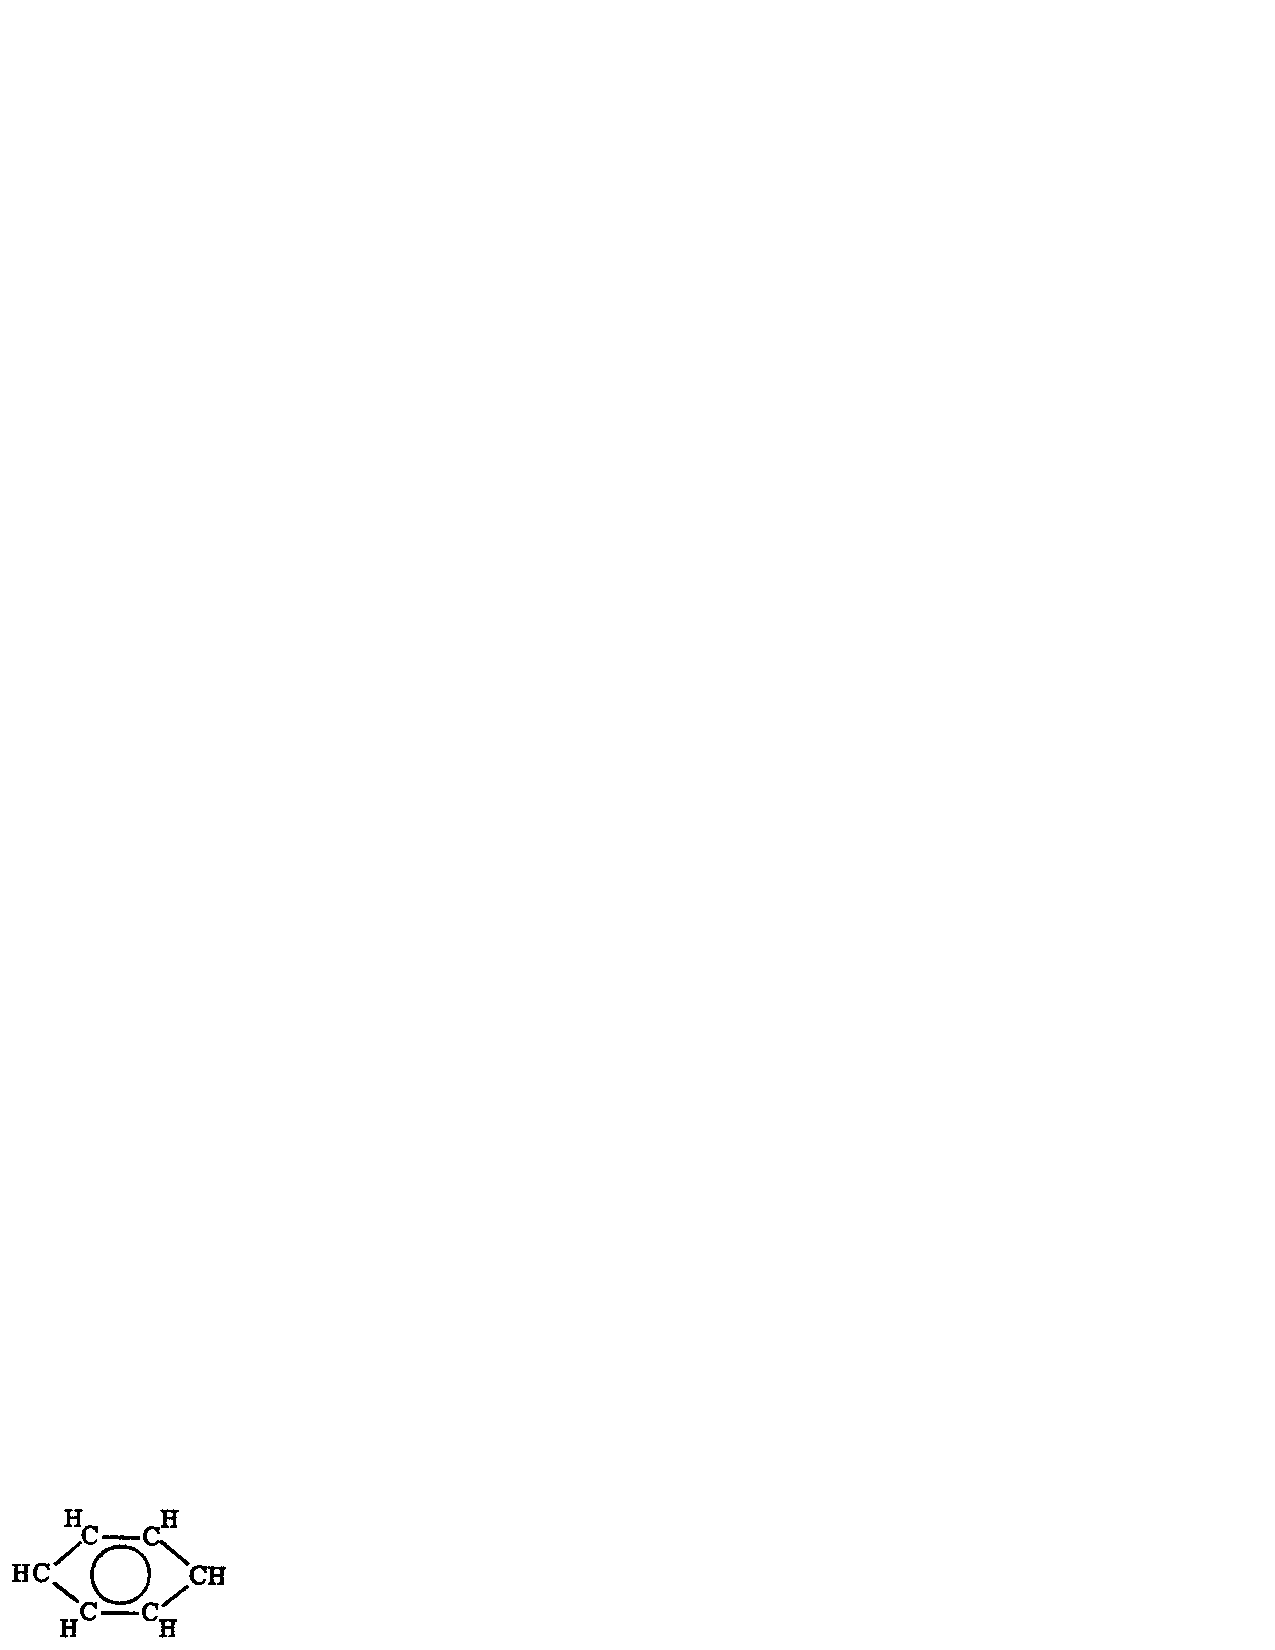
\includegraphics{fg7-10f}
\label{chap7-eqno54}
\end{equation}
Calculations show that the superposition wavefunction $\chi_3$ is 20 kcal 
lower in energy than either $\chi_{2a}$ or $\chi_{2b}$, using the same 
geometry.  This stabilization due to superposition of equivalent bonding 
configurations is referred to as resonance.

In thermonuclear calculations, it is necessary to assume that 
benzene is about 30 to 36 kcal more stable than a kekule line structure.

\subsection{Allyl Radical}

Removing an H from the methyl group of propane
\begin{equation}
% missing figure from p 7-38
%\includegraphics{fg7-}
\end{equation}
leads to allyl radical, a planar molecule with two equivalent 
bonding structures
\begin{equation}
% missing figure from p 7-39
%\includegraphics{fg7-}
\label{chap7-eqno55}
\end{equation}
The $\pi$ part of the wavefunctions, are
\begin{equation}
\chi_{4a} = A \left[ \pi_{\ell} \pi_c \pi_r \left( \alpha \beta - 
\beta \alpha \right) \alpha \right]
\end{equation}
\begin{equation}
\chi_{4b} = \left[ \pi_{\ell} \pi_c \pi_r \alpha \left( \alpha \beta - \beta 
\alpha \right) \right]
\end{equation}
However, the superposition
\begin{equation}
\chi_{(5)} = \chi_{4a} - \chi_{4b} = A \left[ \pi_{\ell} \pi_c \pi_r 
\left( 2 \alpha \beta \alpha - \beta \alpha \alpha - \alpha \alpha 
\beta \right) \right]
\label{chap07-eqno56}
\end{equation}
is more stable by 17 kcal.  Again, this is referred to as the resonance energy.

\subsection{Graphite}

Now we consider a generalization of benzene and allyl, with an 
infinite planar network containing a $\sigma$ bond from each C to three
others
\begin{equation}
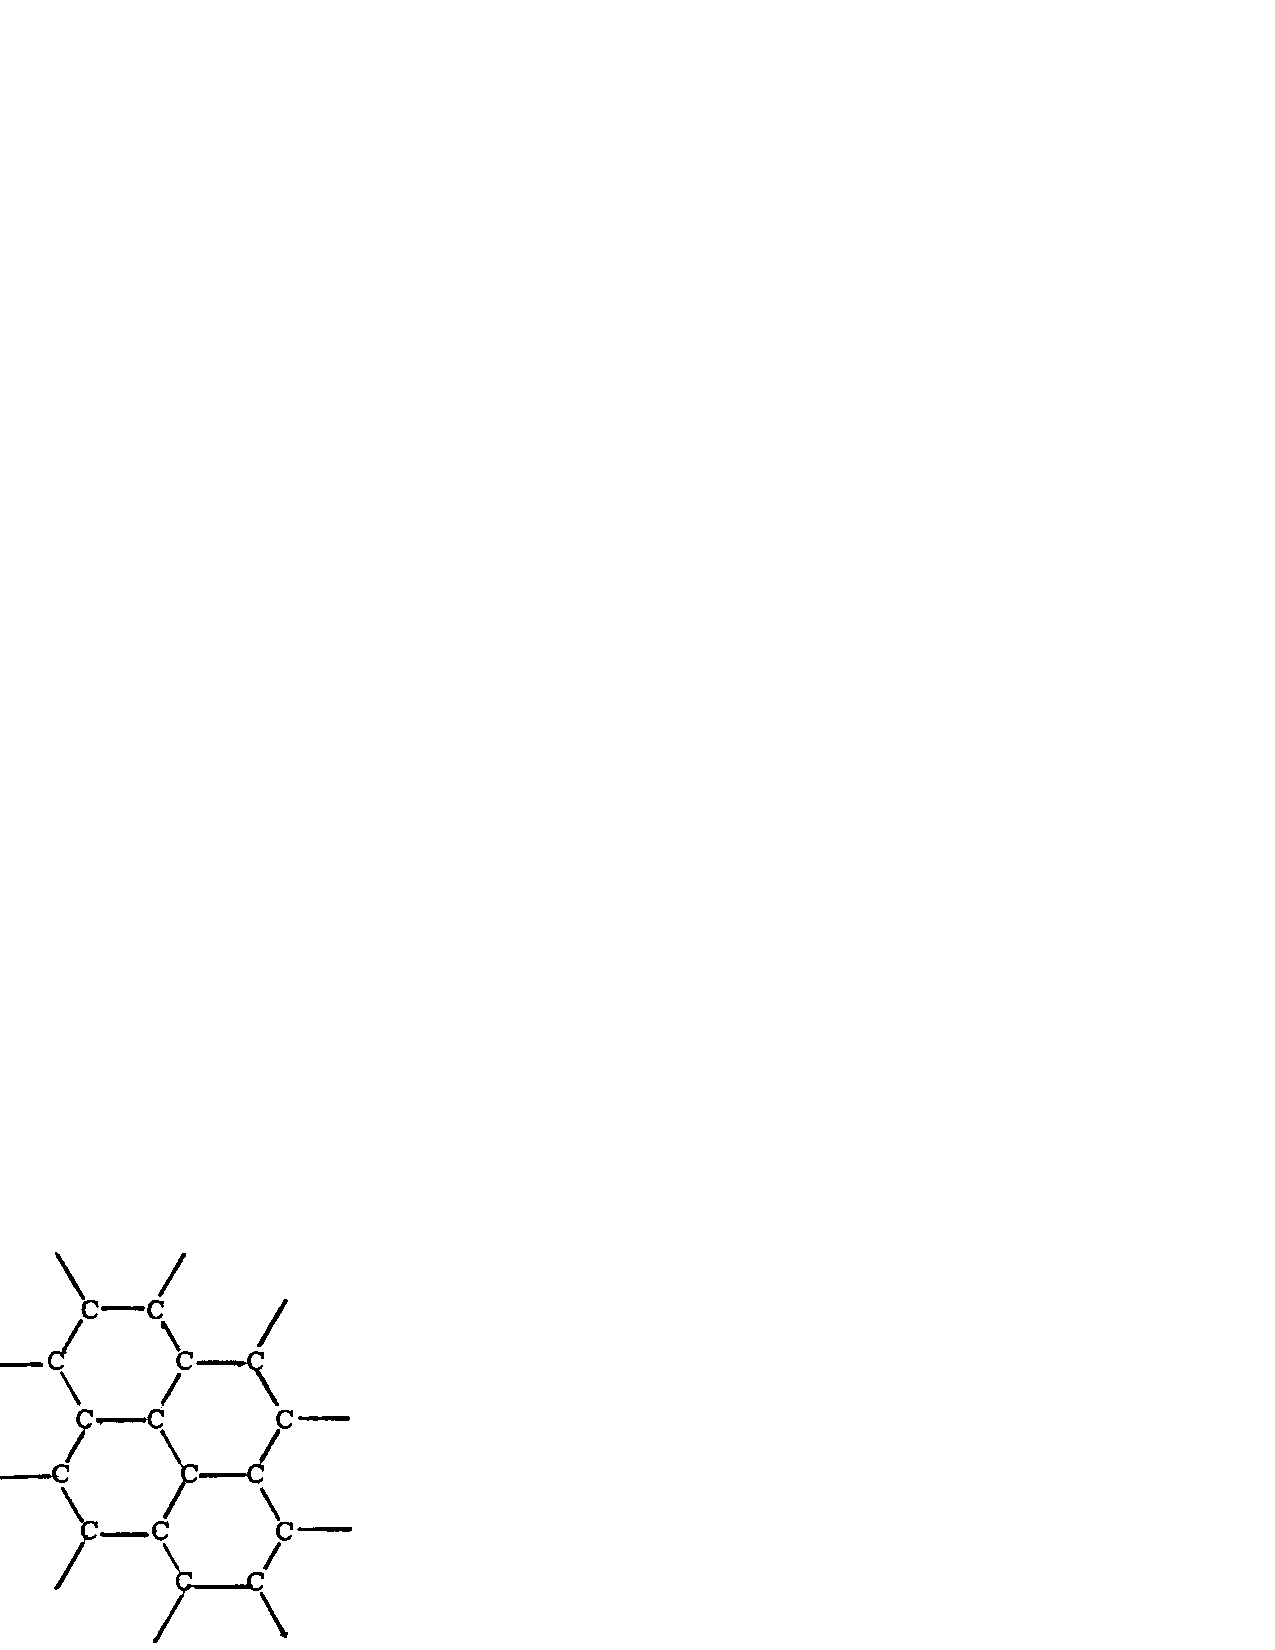
\includegraphics{fg7-10g}
\label{chap7-eqno57}
\end{equation}
This leaves one electron on each C in a $p$ $\pi$ orbital. These $\pi$ orbitals 
can then be paired in many ways, e.g.,
\begin{equation}
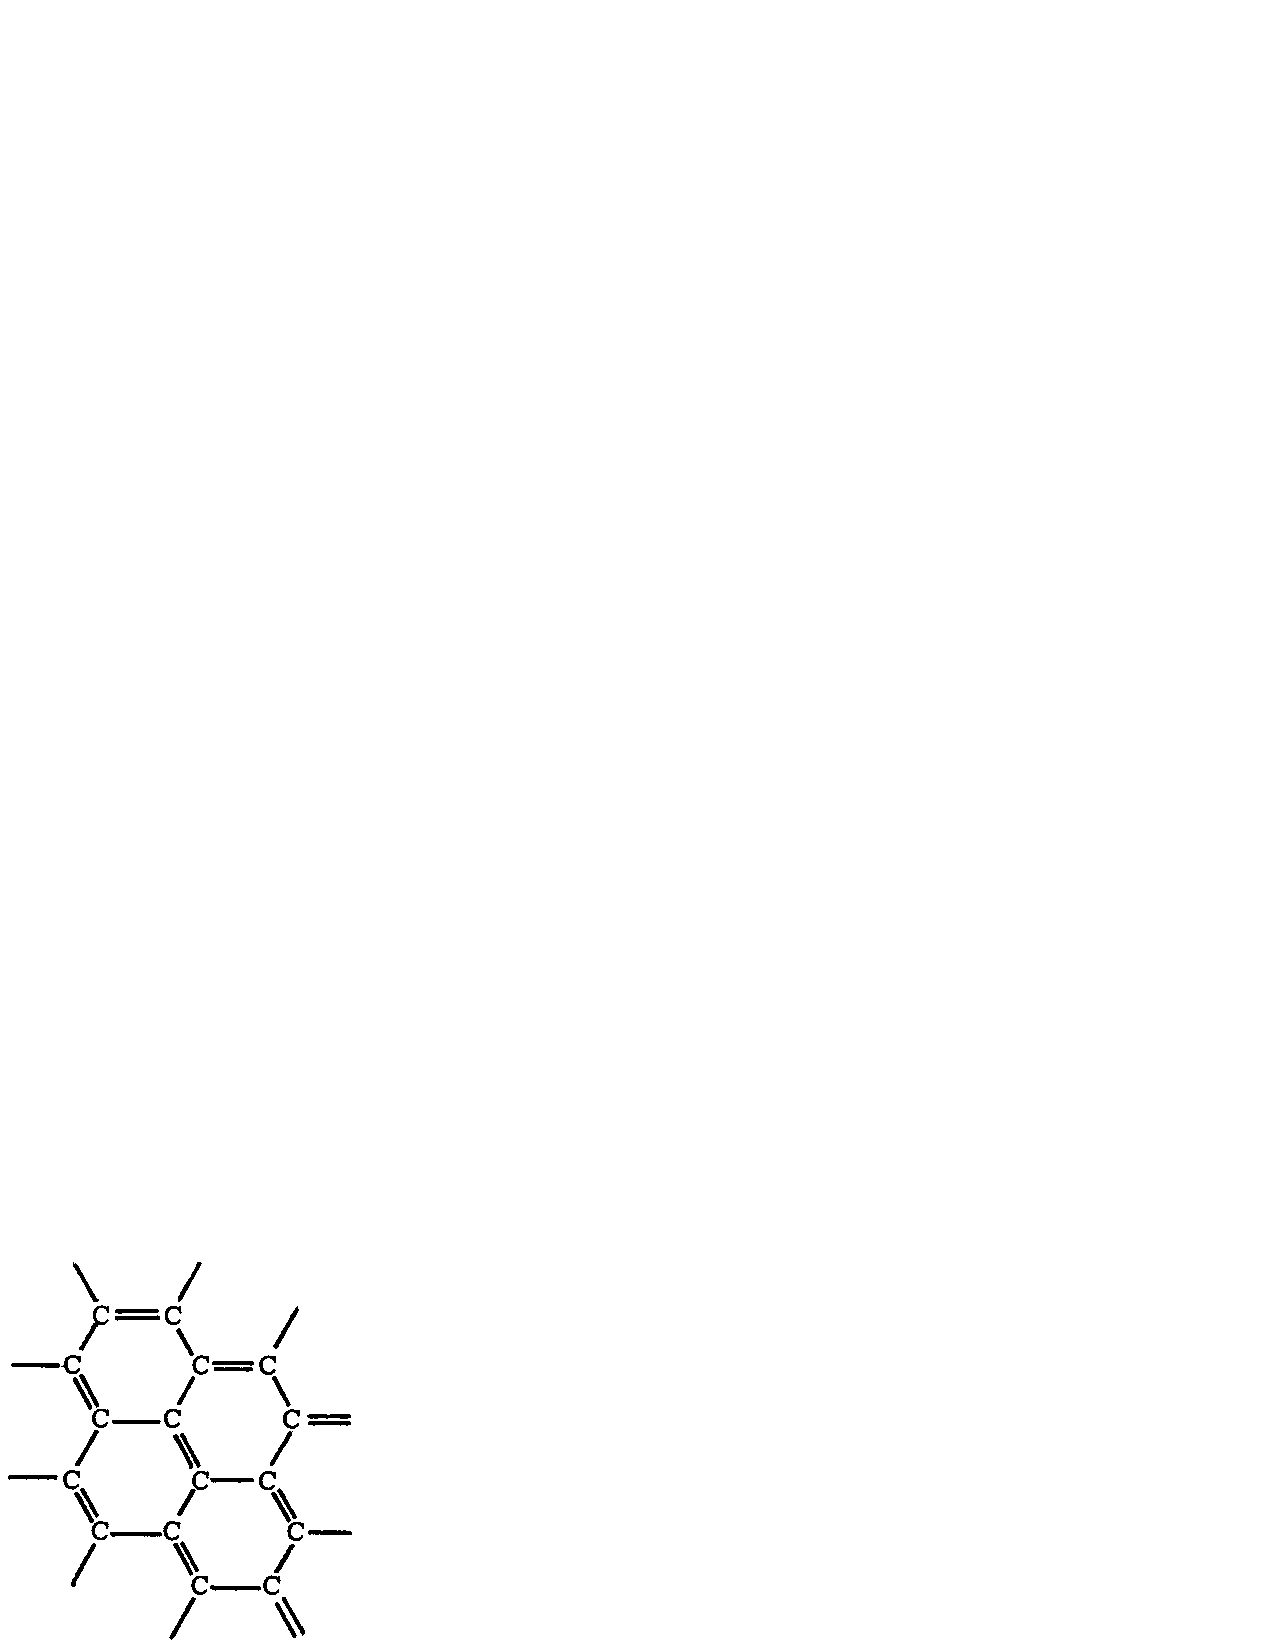
\includegraphics{fg7-10h}
\label{chap7-eqno58}
\end{equation}
and allowing all possible resonance structures for the $\pi$ system,
leads to equivalent bond lengths.  The result is one layer of the 
graphite crystal, the stable form of carbon. In graphite these 
layers are stacked ABAB... where the atoms of the A and B layers 
are oriented as follows, x for A, o, for B
\begin{equation}
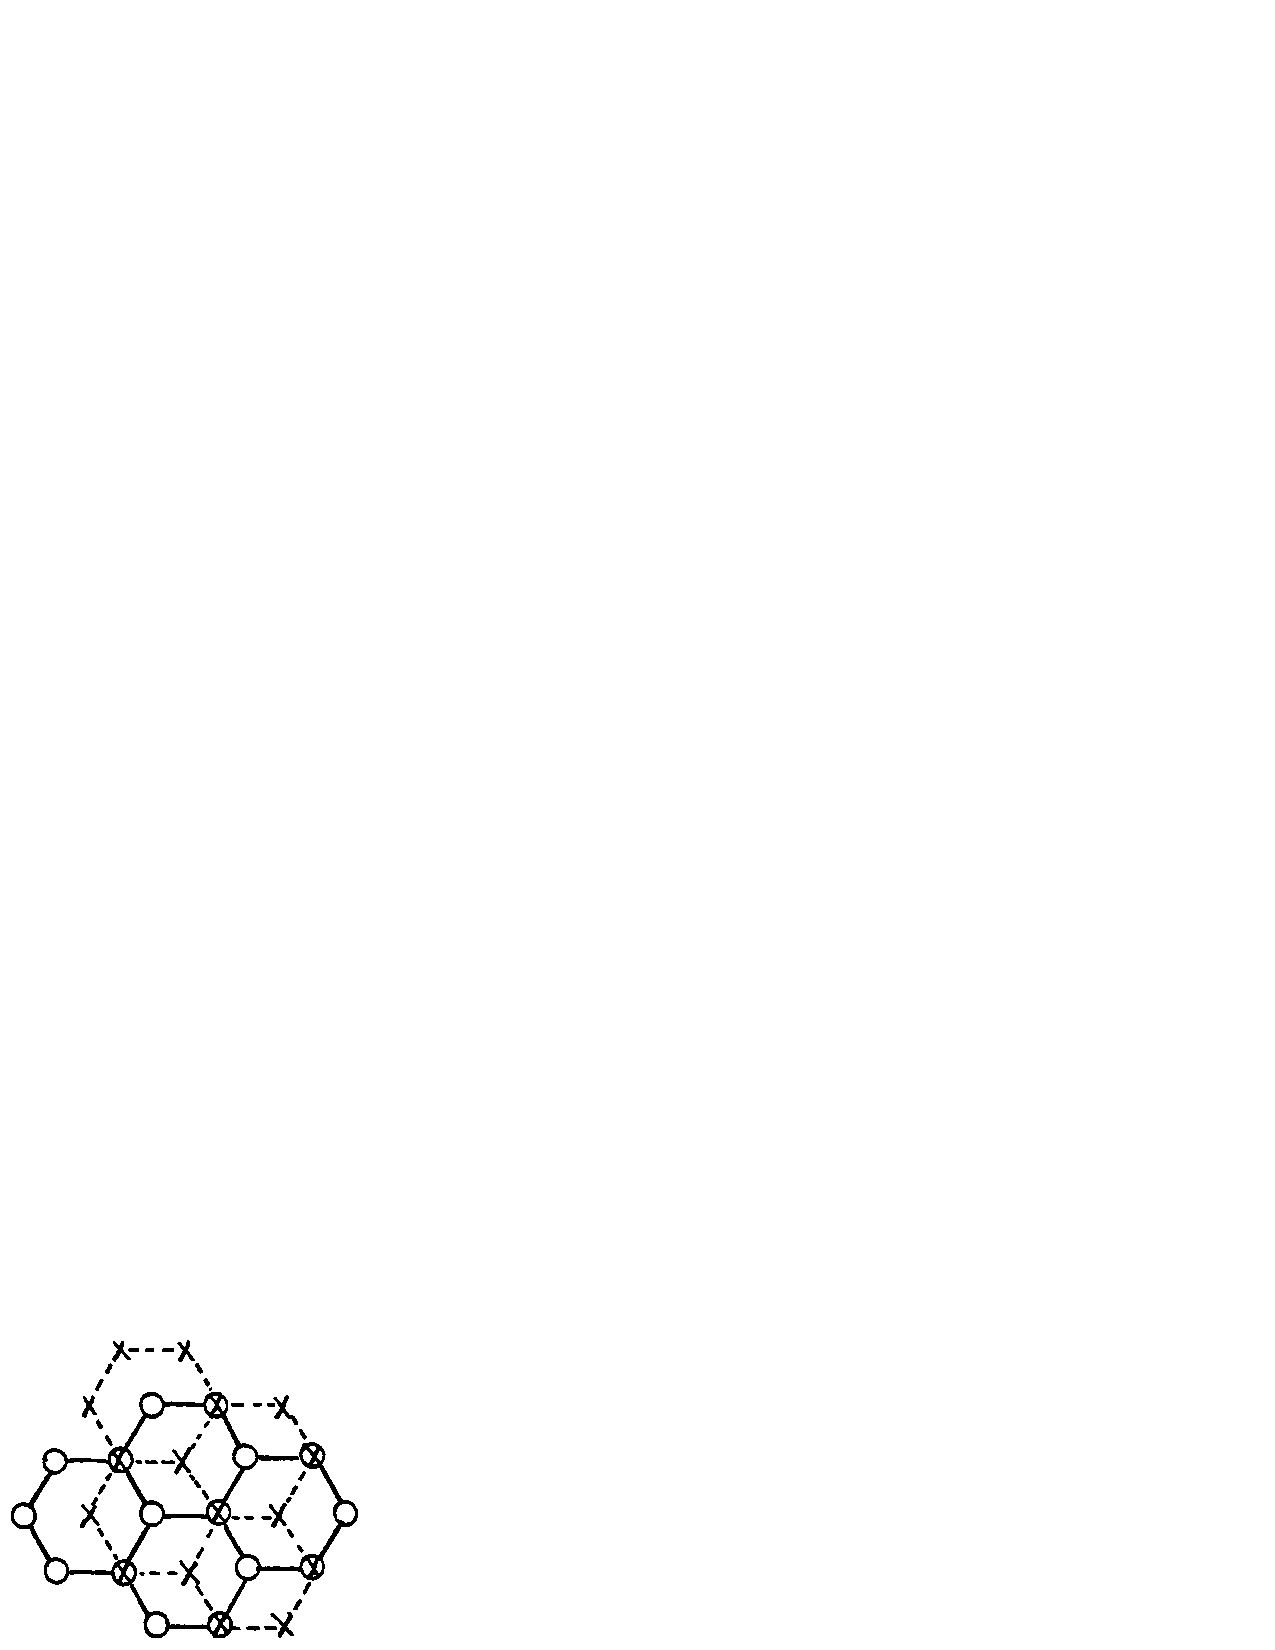
\includegraphics{fg7-10i}
\label{chap7-eqno59}
\end{equation}
The distance between layers is 3.3545 $\pm$ 0.0006 \AA, while 
the C-C bond length within a layer is 1.4210 $\pm$ 0.0002 \AA.  There 
are only weak forces between layers, so that it is very easy for 
these layers to be slid with respect to each other. As a result, 
graphite is used as a lubricant.

On the average there is one-third of a $\pi$ bond for each C-C $\sigma$ bond 
in graphite. This can be compared to diamond with a single 
sigma bond, to ethylene with a double bond,
\begin{equation}
% missing figure from p 7-41
\end{equation}
to acetylene with a triple bond
\begin{equation}
% missing figure from p 7-41
\end{equation}
and to benzene (\ref{chap7-eqno37}) with a sesqui bond, $n = 3/2$,
between each pair of carbons.

Although graphite is the ground state of carbon, at normal 
atmospheric pressure, the energy difference between graphite 
and diamond is quite small.  At 0$^{\circ}$K the enthalpy of diamond 
is 0.580 kcal higher than that of graphite.

\section{C$_n$}

The ground state of C$_3$ is
\begin{equation}
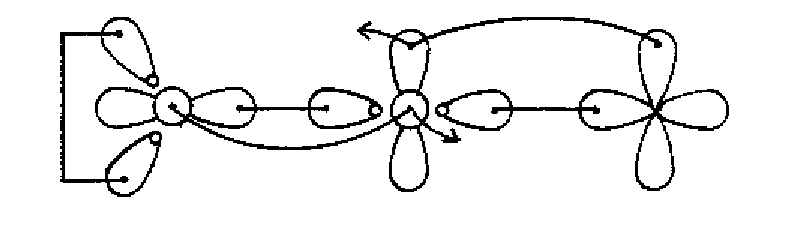
\includegraphics{fg7-10j-1}
\label{chap7-eqno60}
\end{equation}
the lobe pair on the right C is out of the plane, and not shown, while 
C$_4$ is
\begin{equation}
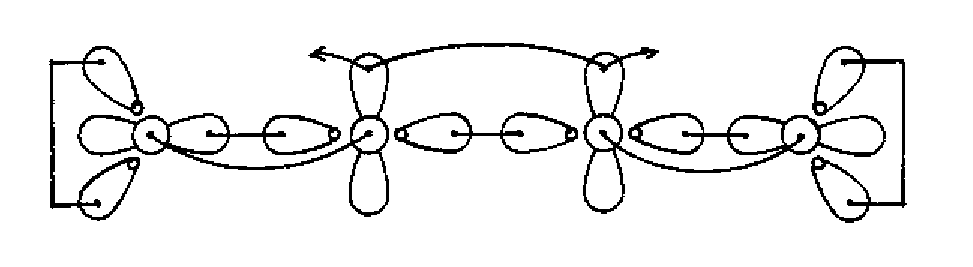
\includegraphics[scale=0.75]{fg7-10j-2}
\label{chap7-eqno61}
\end{equation}
and C$_5$ is
\begin{equation}
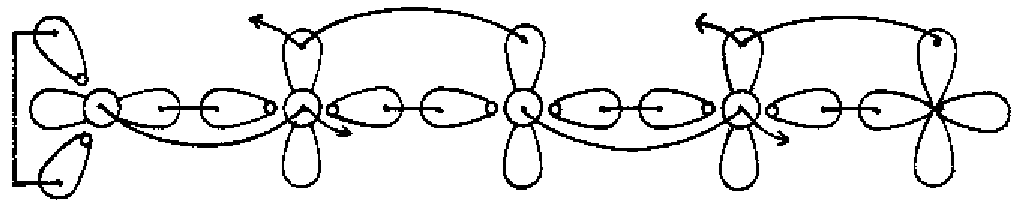
\includegraphics[scale=0.75]{fg7-10j-3}
\label{chap7-eqno62}
\end{equation}
(right lobe pair not shown).  The energies of these species are
summarized in Table \ref{chap7-tab7}, where we see that the bond
energy to form an odd C$_n$ is $\sim$33 kcal larger than that for an
even C$_n$.  Probably this is because odd C$_n$ has an empty $\pi_x$
orbital on one terminus, and an empty $\pi_y$ orbital on the other
terminus.  Allowing stabilization of both $\pi$ systems, $\pi_x$ and
$\pi_y$, by delocalizing concertedly into the empty $\pi$ orbitals.
Whereas, for odd C$_n$, the empty $\pi$ orbitals are both in the same
plane, allowing stabilization of only one $\pi$ system.

\begin{table}
\caption{Cohesive and incremental energy.}
\label{chap7-tab7}
\begin{tabular}{ccccc}\\ \hline

& $\Delta H_{fo}$$^a$ &\multicolumn{2}{c}{Cohesive Energy}
&Incremental Energy\cr
& & Total & Bond\cr
& (kcal) & (kcal) & per atom\cr

C$_1$ &	169.6 & 0 & 0 & 0\cr
C$_2$ &	198.2 & 141.0 & 70.5 & 141.0\cr
C$_3$ & 194 & 319.8 & 104.9 & 173.8\cr
C$_4$ &	230.4 & 448.0 & 112.0 & 133.2\cr
C$_5$ &	232.4 & 615.6 & 123.1 & 167.6\cr
Graphite & 0.0 & & 169.6\cr
\hline
\end{tabular}\\
$^a$See reference 6.
\end{table}

\begin{table}
\caption{Fraction of C$_n$ species in vapor over graphite.}
\label{chap7-tab8}
\begin{tabular}{cccccc}\\ \hline

& C$_1$ & C$_2$ & C$_3$ & Higher & Total $p$\cr
& & & & C$_n$ & Atom\cr

$T = 1000^{\circ}$K & 0.987 & 0.0002 & 0.013 & & $5.2 \times 
10^{-30}$\cr
$T = 2000^{\circ}$K & 0.500 & 0.058 & 0.433 & 0.008 & $6.0 \times 
10^{-11}$\cr
$T = 3000^{\circ}$K & 0.019 & 0.160 & 0.542 & 0.279 & $2.6 \times 
10^{-4}$\cr
$T = 4000^{\circ}$K & 0.106 & 0.235 & 0.497 & 0.162 & 1.0\cr
\hline
\end{tabular}
\end{table}

In consequence, we find the following enthalpy changes for 
disproportionation 
\begin{eqnarray}
2C_2 & \rightarrow& C_1 + C_3 ~~ \Delta H = - 32.8 ~ {\rm kcal}\cr
2C_3 & \rightarrow& C_2 + C_4 ~~ \Delta H = + 40.6\cr
2C_4 & \rightarrow& C_3 + C_5 ~~ \Delta H = -34.4
\end{eqnarray}
Thus, we expect odd C$_n$ to dominate in carbon vapors, a result that is
observed, see Table \ref{chap7-tab8}. 

At some point it should be favorable to bend C$_n$ to form a ring molecule,
e.g.,
\begin{equation}
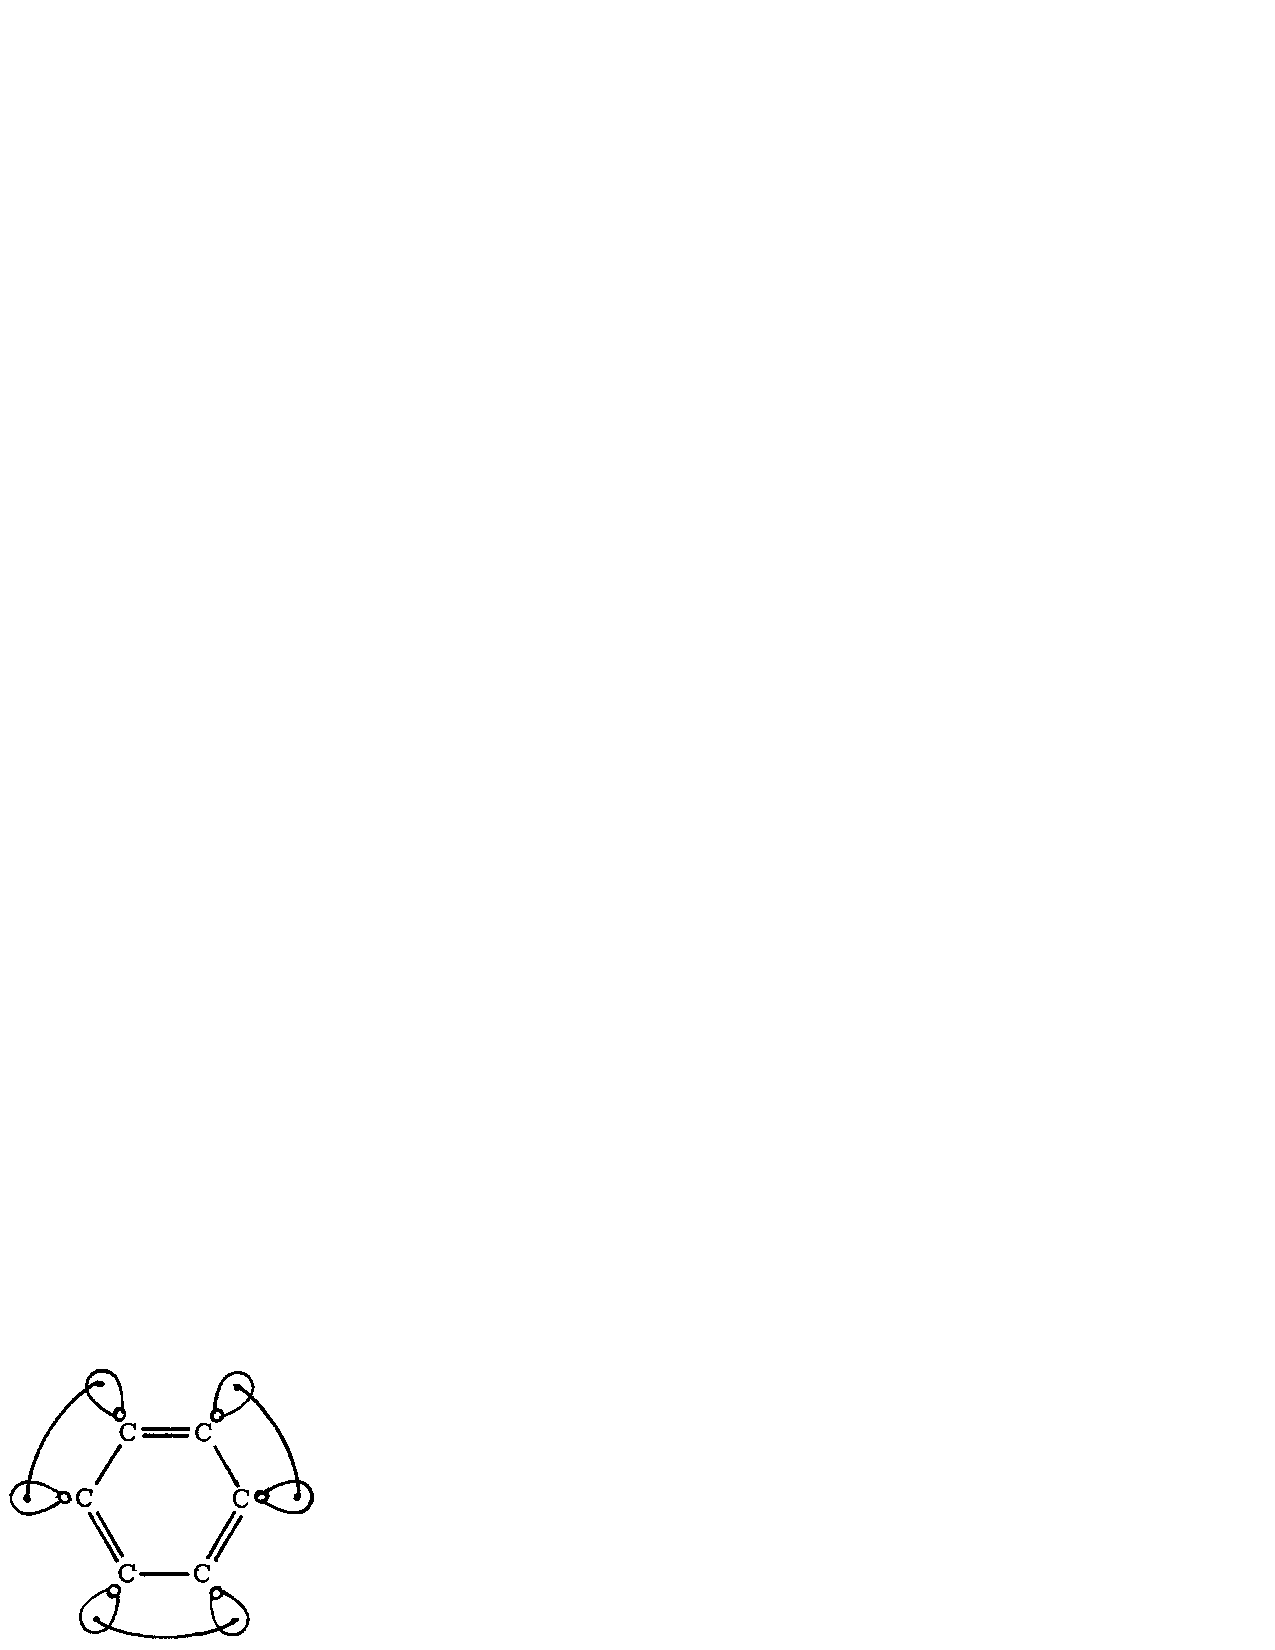
\includegraphics{fg7-10k}
\label{chap7-eqno63}
\end{equation}

Such a species, may be involved in forming the nuclei leading to 
soot formation in flames and engines.

\section{Bond Distances}

\subsection{CC Bond Lengths}

\begin{table}
\caption{Carbon-carbon bond lengths, in \AA, mainly 
from microwave and X-ray diffraction studies.}
\label{chap7-tab9}
\begin{tabular}{cccc}\\ \hline

CC Single Bonds & 1.5445 & diamond\cr
& 1.526 & ethane\cr
& 1.501& \chem{MeCHO}\cr
& 1.49 $\pm$ .01 & \chem{HOOC-COOH}\cr
& 1.488 & \chem{MeCH=CH2}\cr
& 1.472 & epoxide\cr
& 1.470 & \chem{CH2=CH-CHO}\cr
& 1.464 & \chem{CH2=CMe-MeC=CH2}\cr
& 1.459 & Me$-$C$\equiv$CH\cr
& 1.458 & Me$-$C$\equiv$N\cr
& 1.445 & \chem{HC\equiv C-CHO}\cr
& 1.410 & twisted ethylene\cr
& 1.389 & NC$-$CN\cr
& 1.378 & NC$-$C$\equiv$CH\cr
& 1.376 & HCC$-$CCH\cr
Intermediate Bonds & 1.4210 & Graphite, $n = 4/3$\cr
& 1.397 & Benzene, $n = 3/2$ \cr
CC Double Bonds & 1.353 & allyl\cr
& 1.339 & ethylene\cr
& 1.337 & \chem{CH_2=CH-CH=CH_2}\cr
& 1.315 & H$_2$C=C=O\cr
& 1.3084 & H$_2$C=C=CH$_2$\cr
& 1.277	& :C=C=C:\cr
CC Triple Bonds & 1.209 & \chem{HC\equiv CCHO}\cr
& 1.208 & acetylene\cr
& 1.206 & HC$\equiv$C$-$Me\cr
& 1.206	& Me$-$C$\equiv$C$-$C$\equiv$C$-$Me\cr
C$_2$ States & 1.2425 & ${^1\Sigma}_g$\cr
& 1.23 & ${^3\Sigma}_u$\cr
& 1.3119 & ${^3\Pi}_u$\cr
& 1.3693 & ${^3\Sigma}^-_g$\cr
\hline
\end{tabular}
\end{table}

In Table \ref{chap7-tab9} we list various carbon-carbon bond lengths.
For C-C single bonds the variation is 0.17 \AA.  Just as with bond
energies, we can interpret these variations in terms of a decrease in
nonbonded repulsions, which are maximal for C$_2$H$_6$ and diamond,
and minimal for NC-CN, NC-CCH, and HCC-CCH.  As expected from such an
interpretation, there is little variation in the lengths of triple
bonds.  Similarly this interpretation is consistent with the sequence
of double bonds.

A test of this interpretation is to compare with the bond lengths of 
C$_2$.  As shown in Chapter 8, the ${^1\Sigma}^+_g$ and 
${^3\Sigma}^+_u$ states of C$_2$ have the character
\begin{equation}
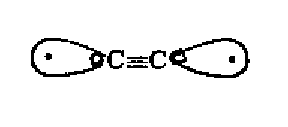
\includegraphics{fg7-10l-1}
\end{equation}
differing only in the spin pairing of the two nonbonding orbitals.  These 
states lead to $R_{CC} = 1.24$ \AA, only slightly larger than the 1.21 
\AA\ found for acetylene.  On the other hand, the ${^3\Sigma}^-_g$ state 
can be considered as having a double bond, leading to $R_{C=C} = 
1.32$ \AA, in reasonable 
agreement with the values 1.31 \AA\ from Table \ref{chap7-tab9}.

In order to isolate the factors determining bond lengths, it is useful 
to compare cases with comparable geometrical constraints.  For example, 
there are a number of systems in which two adjacent carbons are 
trigonal and in the same plane,
\begin{equation}
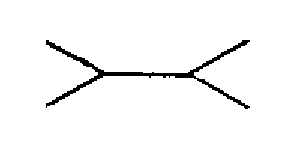
\includegraphics{fg7-10l-2}
\end{equation}
(one might refer to this as $sp^2 - sp^2$ bonding).  This includes:
ethylene $n = 2$; benzene $n = 3/2$; graphite $n = 4/3$; and, the
central bond of butadiene, $n = 1$.  As shown in Figure
\ref{chap7-fig11}, the variations in bond lengths is nearly linear.
\begin{figure}
% Warning: bad figure. Need to rescan p 7-48
%\includegraphics[scale=0.75]{fg7-11}
\caption{C-C bond length versus bond order.  The vertical lines at $n
= 1$ and $n = 2$, represent the range of values know for various
compounds (see Table \ref{chap7-tab9}).  The solid line through the
points connects species with $sp^2 - sp^2$ carbon-carbon bonds. The
dashed line is Pauling's formula (refitted to current values).}
\label{chap7-fig}
\end{figure}

In particular, we see that the CC bond length of benzene is 
the average of the C=C and C$-$C bond lengths, so that the kekule structure
\begin{equation}
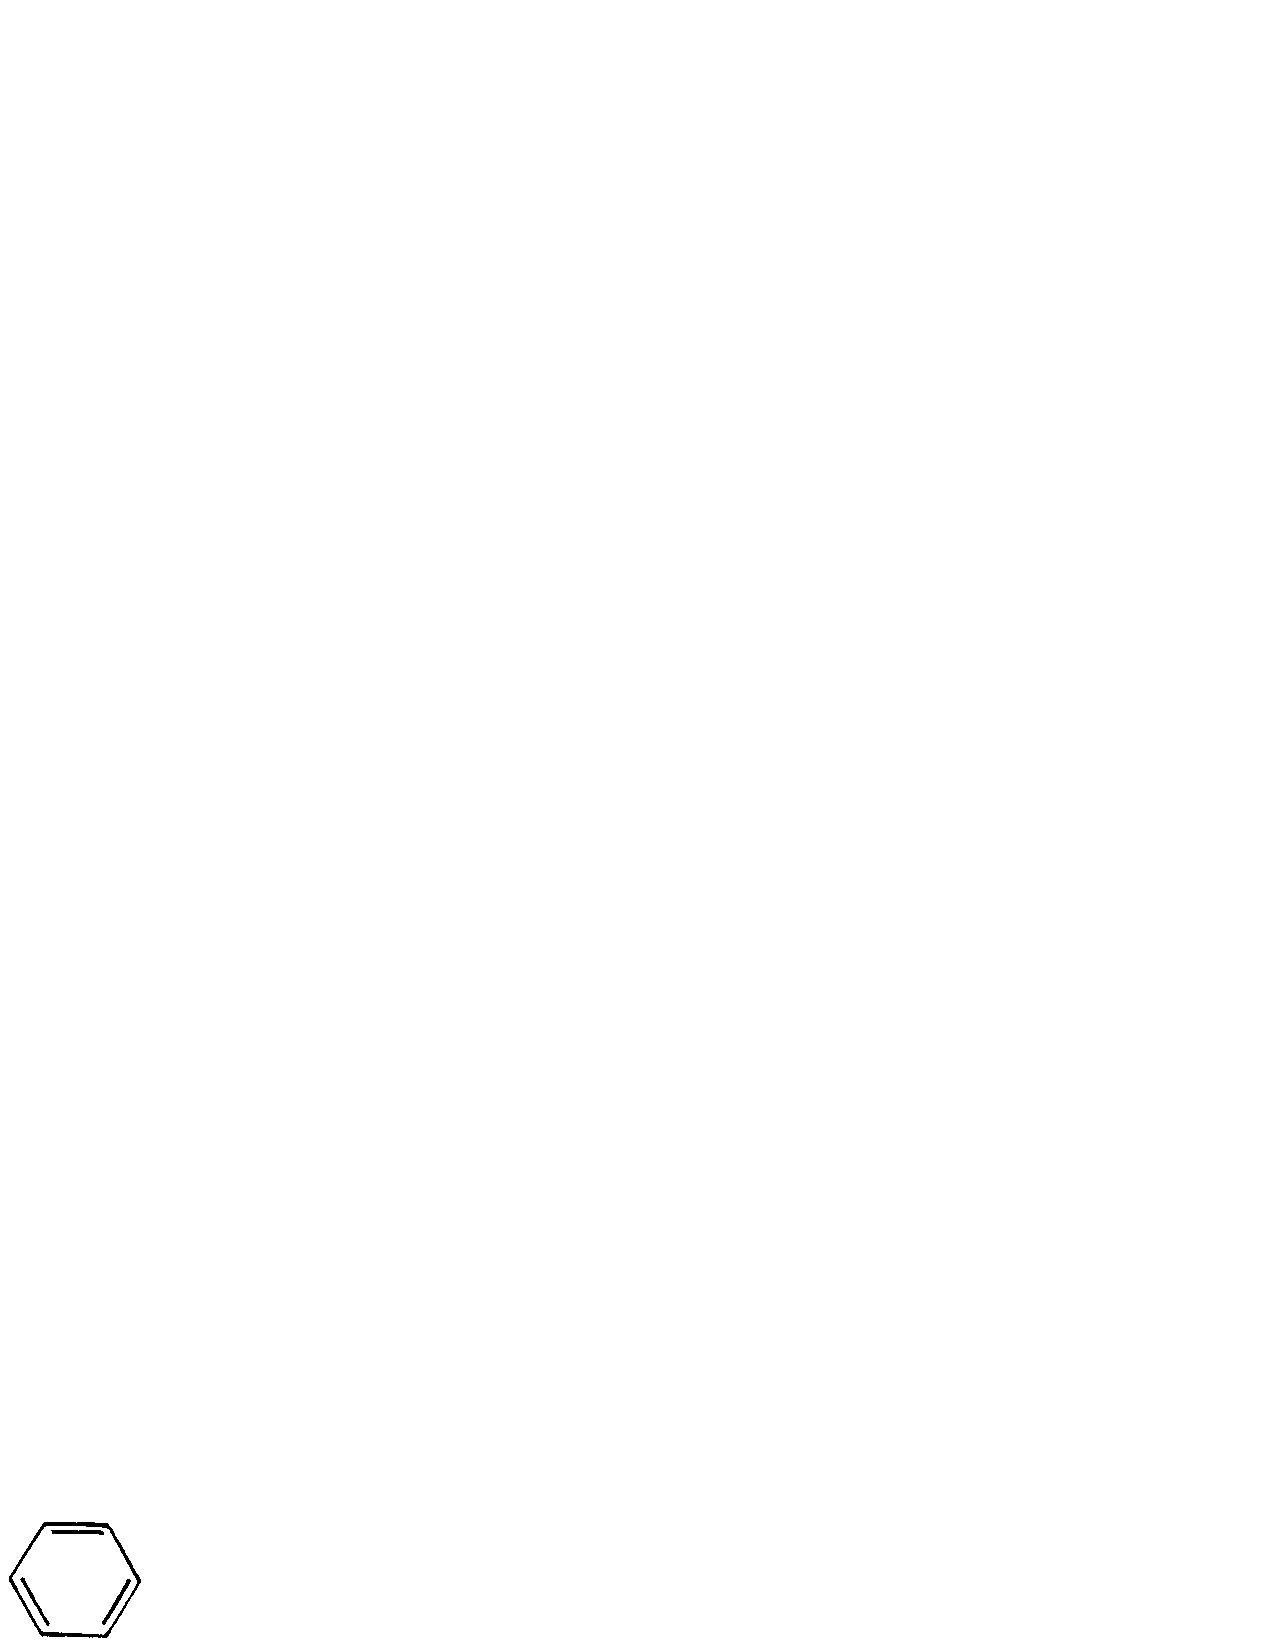
\includegraphics{fg7-10o}
\end{equation}
is expected to have the same perimeter as benzene.

However, the CC bond lengths of ethane, CC = 1.526 \AA, ethylene, 
CC = 1.339 \AA, and acetylene, CC = 1.208 \AA, do not scale 
linearly.  Given the linear scaling found above, for cases 
with similar geometries, my belief is that this nonlinearity 
is due to nonbonded repulsions which are inordinately worse 
for single CC bonds.
	
An alternative explanation was provided by Pauling, who 
suggested, from considering the variation of bond lengths 
for diamond, ethylene, and acetylene, that the bond length, $R_n$  
and bond order, $n$, are related by$^3$
\begin{equation}
R_n = 1.542 - 0.71 \log n
\label{chap07-eqno64}
\end{equation}
using current experimental programs for diamond and acetylene,
(\ref{chap7-eqno64}) becomes
\begin{equation}
R_n = 1. 544 - 0.704 \log n
\end{equation}
leading to $R_{CC} =$ 1.332 \AA\ for ethylene, experimental 1.339. 
Using this formula for benzene, predicts $R_{CC} =$ 1.4209,	whereas the
experimental value is $R = 1.397$ \AA.  A similar discrepancy occurs 
for graphite, $R^{calc} = 1.4569$, $R^{exp} = 1.421$.  Pauling suggested 
that resonance effects are responsible for the additional 
decrease in the bond length.

\subsection{CH Bond Lengths}

\begin{table}
\caption{CH bond lengths.  For cases with more than one CH bond, it is
the left one that is being considered.}
\label{chap7-tab10}
\begin{tabular}{ccc}\\ \hline
$R_{CH}$ & Relevant Bond Angle & \cr
1.120 & HCOl: 103.4\cr
1.114 & CCO: 123.9\cr
1.113 & HCH: 110.5 & Me$-$Cl\cr
1.11 &\cr
1.106 &\cr
1.105 & HCH: 110.2 & Me$-$C$\equiv$CH\cr
1.104 & & Me$-$CN\cr
1.102 & HCH: 121.1\cr
1.097 & HC=O: 111\cr
1.095 & HCO: 127.3\cr
1.094 & & H$-$Me\cr
1.091 & BCH: 108.0 & ethane\cr
1.087 & BCH: 118.2 & H$_2$C=C$-$CH$_2$\cr
1.086 & HCH: 117.6 & ethylene\cr
1.086 & HCH: 108.3\cr
1.084 & & benzene\cr
1.082 & HCH: 116.7\cr
1.080 & HCH: 127 & H$_2$CNN\cr
1.079 & HCH: 122.3\cr
1.079 &\cr
1.071 &\cr
1.058 & & H$-$C$\equiv$CH\cr
1.058 & & H$-$C$\equiv$C$-$CN\cr
1.056 & & H$-$C$\equiv$C$-$Me\cr
1.055 &\cr
\hline
\end{tabular}
\end{table}

Table \ref{chap7-tab10} lists CH bond lengths for various systems.
They vary in a way consistent with non-bonded repulsions.

\section{Bond Energies and Thermochemical Calculations}

In examining reaction mechanisms, Chapter 11, it is often 
necessary to estimate the energies of reaction intermediates.  In 
making these estimates, it is useful to have a good understanding 
of the magnitudes of various bond energies and their trends with 
changes in substituents.  Some of the trends in bond energies will 
be discussed.

More commonly, the energies of molecules are tabulated in terms 
of the enthalpy at standard temperature, 298.15$^{\circ}$K, and pressure, 
760 torr = 1 atmosphere, and estimates of these quantities will 
occupy the balance of this section.  Of course, the zero of energy 
for a system is arbitrary.  In quantum mechanical studies, we usually 
assign zero energy to the state in which all electrons and nuclei 
are infinitely separated from each other.  In the chemical 
literature, the zero of enthalpy is assigned to the equilibrium 
state of each pure substance at 298.15$^{\circ}$K and atmospheric 
pressure.  Using this zero, the enthalpy of any material is 
referred to as the heat of formation, and denoted as $\Delta H^0_f$, 
which is a function of temperature and, hence, $\Delta H^0_{fT}$ is
sometimes used, we will usually use $T = 298.15^{\circ}$K and omit 
$T$.  For carbon the standard state is graphite, for hydrogen the 
standard state is gaseous H$_2$
and for oxygen the standard state is gaseous O$_2$.  The most accurate 
$\Delta H^0_f$ for other molecules are obtained by combustion of the 
material to CO$_2$ and H$_2$O.  For radicals, the situation is
much more difficult, but for many cases, e.g., CH$_3$, CH$_2$, 
CH, and H, accurate values have been obtained using 
spectroscopic and photoionization techniques.  The $\Delta H_f$
for a number of molecules are given in Table \ref{chap7-tab11}.

\begin{table}
\caption{Heats of formation for various (gaseous) molecules.}
\label{chap7-tab11}
\begin{tabular}{cccccc}\\ \hline

& & 0$^{\circ}$K & 298.15$^{\circ}$K Source\cr

Radicals &  H($^2S$) & 51.631 & 52.100 & c,e\cr
& C($^3P$) & 169.58 & 170.89 & c\cr
& CH$_2$($^2B_1$) & 92.25 & 92.07 & c,b\cr
& Me=CH$_3$($^2A^{\prime \prime}$) & 35.62 & 34.82 & c,a\cr

& Et=Me & & 26.7 & h\cr

& n-Pr=Et & & 22.0 & h\cr

& i-Pr=H & & 18.8 & h\cr

& s-Bu=H & & 14.4 & h\cr

& t-Bu=Me & & 9.3 & h\cr

& $V_y =$ & & 69 & g\cr
Alkanes & CH$_4$ & $-$15.99 & $-$17.895 & c\cr
& C$_2$H$_6$ & & $-$20.24 & f,i\cr
& Propane & & $-$24.83 & i\cr
& n-Butane & & $-$ 30.36 & i\cr
& iso-Butane & & $-$32.41 & i\cr
& n-Pentane & & $-$35.10 & i\cr
& iso-Pentane & & $-$36.85 & i\cr
& neo-Pentane & & $-$40.27 & i\cr
& n-Hexane & & $-$39.92 & i\cr
Alkenes & C$_2$H$_4$ & 14.59 & 12.54 & c\cr
& propene & & 4.88 & f\cr
& But-1-ene & & $-$0.03 & f\cr
& Cis-But-2-ene & & $-$1.67 & f\cr
& Trans-But-2-ene & & $-$2.67 & f\cr

Others & 1,3-Butadiene & & 26.33 & f\cr
& C$_2$H$_2$ & 54.33 & 54.19 & c\cr
& benzene & & 19.32 & f\cr
Cyclic & Cyclopropane & & 12.74 & f\cr
& Methylenecyclopropane & & 48.0 & f\cr
& Cyclopropene & & 66.6 & f\cr
& Cyclobutane & & 6.4 & f\cr
& Cyclobutene & & 37.5 & f\cr
& Cyclohexane & & $-$29.43 & f\cr
& Cyclohexene & & $-$0.84 & f\cr
& 1,3-Cyclohexadiene & & 26.0 & f\cr
& 1,4-Cyclohexadiene & & 26.3 & f\cr
& Bicyclo[1.1.0] Butane & & 51.9 & f\cr

\hline
\end{tabular}\\
$^a$The photoionization spectrum of CH$_4$ and onset of 
CH$^+_2$ production leads to $D_0(H-CH_3)=103.24 \pm 0.12$ kcal. 
W. A. Chupka, in J. Chem. Phys., volume 48, page 2337, 1968.
$^b$Using photoionization threshold for production of CH$^+_2$ 
from CH$_3$ and the IP of CH$_3$, leads to $D_0(H-CH_2) = 108.25 \pm 0.77$ 
kcal.
$^c$JANAF Thermochemical Tables, NSRDS-NBS 37. 
$^d$Spectroscopic, from rotational predissociation of CH.
$^e$Spectroscopic, from $D_0$ of H$_2$. 
$^f$S. W. Benson, F. R. Cruickshank, D. M. Golden, G. R. Haugen, 
H. E. O'Neal, A. S. Rodgers, R. Shaw, and R. Walsh, in Chem. 
Rev., volume 69, page 279, 1969. 
$^g$S. W. Benson, in Thermochemical Kinetics. 
$^h$Best values obtained by W. A. Goddard, June 1978, from 
comparing $\Delta H_f$ for numerous alkenes and alkanes. 
$^i$Cox and Pilcher.
\end{table}

\subsection{Bond Energies}

\begin{table}
\caption{}
\label{chap7-tab12}
\begin{tabular}{cccccc}\\ \hline
& & $D_{298}$(H-R) & & $D_{298}$(Me-R)\cr

& H-Me & 104.82 & nullary & Me-Me & 89.88\cr

& H-Et & 99.0 & primary & Me-Et & 86.4\cr

& H-nPr & 98.9 & primary & Me-nPr & 87.2\cr

& H-iPr & 95.7 & secondary & Me-iPr & 86.0\cr

& H-tBu & 93.8 & tertiary & Me-tBu & 81.0\cr
\hline
\end{tabular}
\end{table}

In Table \ref{chap7-tab12}, we list the CH bond energies for various
cases.  The major point to note is that the CH bond energy is strongly
affected by how many of the other substituents on the C are alkyl
groups:
\begin{center}
\begin{tabular}{lcl}\\
Nullary & H$-$Me & D = 105 kcal\\
Primary & H$-$Et & D = 99 kcal\\
Secondary & H$-$iPr & D = 96 kcal\\
Tertiary & H$-$tBu & D = 94 kcal\\
\end{tabular}
\end{center}
However, it is believed that these bond energies are not affected 
by the identity of the alkyl group.  Thus, $H-nPr$ is the same as H$-$Et,
\begin{equation}
D(\chem{H-Et}) = D(\chem{H-nPr}) = 99 {\rm kcal}.
\end{equation}
Based on these bond energies, we see that starting with n-butane it is
3 kcal lower energy to form sec-butyl: \chem{H_3C-\dot{C}H-CH_2-CH_3},
than it is to form n-butyl: \chem{H_2{\dot{C}}-CH_2-CH_2-CH_3}.  That
is, a secondary radical center, sec-butyl, is 3 kcal more stable than
a primary radical center, n-butyl.  Alternatively, starting with
1-butene
\begin{equation}
% missing figure, p 7-54
\end{equation}
and adding an H atom, the terminal site, C1, is preferred by 
3 kcal over the internal site, C2.  These types of effects are 
involved, for example, in the preferences embodied in 
Markownikoff and anti-Markownikoff additions to double 
bonds, and can be of critical importance in organic chemistry.

As indicated in Table \ref{chap7-tab12}, similar effects, but less
regular, occur for C-C bonds.

\subsection{Average Bond Energies}

A common way to systematize the heats of formation of various 
substances is in terms of average bond energies, which are 
defined such that the heat of atomization, the energy to 
break the molecule into separated atoms, is equal to the sums 
of the bond energies.  Such average bond energies do not tell
us how much energy is in fact required to break a specific 
bond as can be seen for the case of CH$_4$.

From Table \ref{chap7-tab11}, we obtain:
\begin{eqnarray}
D(\chem{H-CH_3}) &=& \Delta H_f(H) + \Delta H_f(CH_3) - \Delta H_f (CH_4)\cr
&=& 104.8 ~ {\rm kcal ~ at} ~ 298.15^{\circ}{\rm K}\cr
&=& 1-3.2 ~ {\rm kcal ~ at ~} 0^{\circ}{\rm K})\cr
D(\chem{H-CH_2}) &=& 92.07 \pm 52.1 - 34.82\cr
&=& 109.4 ~ {\rm kcal}\cr
D(\chem{H-CH}) &=& 102.0 ~ {\rm kcal}\cr
D(\chem{H-C}) &=& 81.0 ~ {\rm kcal}
\end{eqnarray}
On the other hand, the total enthalpy of atomization of CH$_4$ is 
397.2 kcal, so that the average CH bond energy is 99.3 kcal.

\begin{table}
\caption{Bond energy terms from J. D. Cos and G. 
Pilcher, in Thermochemistry of Organic and Organometallic compounds, 
Academic Press, New York, 1970.}
\label{chap7-tab13}
\begin{tabular}{cc}\\ \hline
E(C-C) & 85.48\cr
E(C-H)$_p$ & 98.19\cr
E(C-H)$_s$ & 97.27\cr
E(C-H)$t$ & 96.53\cr
E(C=C) & 133.00\cr
E(C$_d$-H)$_2$ & 101.10\cr
E(C$_b$-H)$_1$ & 100.53\cr
E(C$_d$-C) & 90.07\cr
E(C$_b$-C) & 88.91\cr
\hline
\end{tabular}
\end{table}

A selected set of such average energies is given in Table
\ref{chap7-tab13}. In order to obtain a reasonable fit, it is
necessary to allow a particular bond energy to depend upon which other
atoms are bonded to the atoms involved.  Thus,
\begin{description}
\item {E(C$-$H)$_p$ =} indicates a CH bond in which the C is bonded to one
C and three H, a primary carbon

\item {E(C$-$H)$_s$ =} indicates a CH bond in which the C is bonded to two
C and two H, a secondary carbon

\item {E(C$-$H)$_t$ =} indicates a CH bond in which the C is bonded to three
C and one H, a tertiary carbon

\item {E(C$_d-$H)$_2$ =} indicates a CH bond in which the C is 
bonded to one C with a double bond and to one H

\item {E(C$_d-$H)$_1'$ =} indicates a CH bond in which the C is 
bonded to one C with a single bond and to one C with a double bond

\item {E(C$_b-$H) =} indicates a CH bond to benzene-like C.
\end{description}
Comparing Tables \ref{chap7-tab13} and \ref{chap7-tab14}, we see some
gross disparities.  For example, in Table \ref{chap7-tab13}, the C=C
double bond energy is 133 kcal, whereas the energy to break the CC
bond of ethylene is 172.3 kcal.  Consequently, average bond energies
such as in Table \ref{chap7-tab13} will be of little use in predicting
the energies to break particular bonds.

\begin{table}
\caption{Table of real bond energies.}
\label{chap7-tab14}
\begin{tabular}{ccc}\\ \hline

& 0$^{\circ}$ & 298.15$^{\circ}$K\cr

D(H-CH$_3$) & 103.2 & 104.8\cr
D(H-CH$_2$) & &  109.4\cr
D(H-CH) & & 102.0\cr
D(H-C) & &  81.0\cr
D(H-C$_2$H$_5$) & & 99\cr
D(H-C$_2$H$_3$) & & 108.5\cr
D(H$_2$) & 103.3 & 104.2\cr
D(H$_3$C-CH$_3$) & & 89.9\cr
D(H$_2$C-CH$_2$) & 169.9 & 171.6\cr
D(HC-CH) & 228.1 & 229.8\cr
D(CH$_3$-C$_2$H$_5$) & & 86.4\cr
D(C$_2$H$_5$-C$_2$H$_5$) & & 84\cr
D(CH$_3$-C$_2$H$_3$) & & 99\cr
D(C$_2$H$_3$-C$_2$H$_5$) & & 96\cr
D(C$_2$H$_3$-C$_2$H$_3$) & & 111.7\cr
\hline
\end{tabular}
\end{table}

\subsection{Group Values}

An alternative scheme to building up, and predicting $\Delta H^0_f$ 
is the method of group values developed by Benson.$^4$  The idea here 
is that by characterizing each atom in terms of the atoms, it is bonded to 
and which order of bond, one can develop an additive scheme accurate to 
$\sim$1 kcal.  A standard $\Delta H^0_f$, also $S^0$ and $C^0_p$, 
is assigned to each group of the molecule in such a way
that summing the $\Delta H^0_f$ of the groups, leads to the total 
$\Delta H^0_f$ of the molecule.  Thus, from $\Delta H^0_f (H_3C-CH_3) = 
-20.24$ kcal we use
\begin{equation}
2\Delta H^0_f \left[ C - (H)_3 (C) \right] = \Delta H^0_f 
(C_2H_6) = - 20.24
\end{equation}
to calculate the group value
\begin{equation}
\Delta H^0_f \left[ C - (H)_3 (C) \right] \equiv -10.12 {\rm kcal}
\end{equation}
for a primary carbon, bonded to one carbon and three hydrogens.
Similarly, from the $\Delta H^0_f$ of propane, $H_3C-CH_2-CH_3$, we use
\begin{equation}
\underbrace{\Delta H^0_f(C_3H_8)}_{-24.82} = \underbrace{2\Delta 
H^0_f[C-(H)_3(C)]}_{-10.12} + \underbrace{\Delta 
H^0_f[C-(H)_2(C)_2]}_{-4.58}
\end{equation}
to calculate $\Delta H^0_f [C -(H)_2(C)_2] = -4.58$ kcal for a secondary 
carbon.  Determining these group values by a fit to a number of 
hydrocarbons, leads to the values in Table \ref{chap7-tab15}.

\begin{table}
\caption{Group values for $\Delta H^0_f$.$^a$  C$_d$ 
refers to a C with a double bond to another C.
C$_t$ refers to a C with a triple bond to another C.
C$_a$ refers to a C with double bonds to two C's.
C$_b$ refers to a C in a benzene ring.}
\label{chap7-tab15}
\begin{tabular}{cc}\\ \hline

C$-$(H)$_3$(C) & $-$10.08\cr
C$-$(H)$_2$(C)$_2$ & $-$~4.95\cr
C$-$(H)(C)$_3$ & $-$~1.90\cr
C$-$(C)$_4$ & ~~ 0.05\cr

C$_d-$(H)$_2$ & ~~ 6.26\cr
C$_d-$(H)(C) & ~~ 8.59\cr
C$_d-$(C)$_2$ & ~ 10.34\cr
C$_d-$(C$_d$)(H) & ~~ 6.78\cr
C$_d-$(C$_d$)(C) & ~~ 8.88\cr
C$_d-$(C$_b$)(H) & ~~ 6.78\cr
C$_d-$(C$_b$)(C) & ~~ 8.64\cr
C$_d-$(C$_t$)(H) & ~~ 6.78\cr

C$_t$(H) & ~ 26.93\cr
C$_t$(C) & ~ 27.55\cr
C$_t$(C$_d$) & ~ 29.20\cr
C$_t$(C$_b$) & ~ 29.20\cr

$C_a$ & ~ 34.20\cr

C$-$(C$_d$)(H)$_3$ & $-$ ~ 9.79\cr
C$-$(C$_d$)(C)(H)$_2$ & $-$ ~ 4.76\cr
C$-$(C$_d$)$_2$(H)$_2$ & $-$ ~ 4.29\cr
C$-$(C$_d$)(C$_b$)(H)$_2$ & $-$ ~ 4.29\cr
C$-$(C$_t$)(C)(H)$_2$ & $-$ ~ 4.73\cr
C$-$(C$_b$)(C)(H)$_2$ & $-$ ~ 4.86\cr
C$-$(C$_d$)(C)$_2$(H) & $-$ ~ 1.48\cr
C$-$(C$_t$)(C)$_2$(H) & $-$ ~ 1.72\cr
C$-$(C$_b$)(C)$_2$(H) & $-$ ~ 0.98\cr
C$-$(C$_d$)(C)$_3$ & ~~~ 1.68\cr
C$-$(C$_b$)(C)$_3$ & ~~~ 2.81\cr

$C_b-$(H) & ~~~ 3.30\cr
$C_b-$(C) & ~~~ 5.51\cr
$C_b-$(C$_d$) & ~~~ 5.68\cr
$C_b-$(C$_t$) & ~~~ 5.68\cr
$C_b-$(C$_b$) & ~~~ 4.96\cr
\hline
\end{tabular}\\
$^a$From S. Benson, in Thermonuclear Kinetics, J. Wiley, 1968.
\end{table}

Some examples of the use of Table \ref{chap7-tab15} follow, ignoring
resonance effects (see the next section):

\begin{enumerate}
\item 1,3-butadiene:
  \begin{enumerate}
  \item $2\times C_d-(H)_2 = 12.52$
  \item $2\times C_d-(C)(H) = 17.18$
  \item $\Delta H_f = 29.7$
  \end{enumerate}
\item 1,3,5-hexatriene:
  \begin{enumerate}
  \item $2\times C_d-(H)_2 = 12.52$
  \item $4\times C_d-(C)(H) = 34.36$
  \item $\Delta H_f = 46.9$
  \end{enumerate}
\item \chem{H_3C-C \equiv C-C \equiv C-CH_3}:
  \begin{enumerate}
  \item $2\times C - (C)(H)_3 = - 20.16$
  \item $4\times C_t - (C) = 110.20$
  \item $\Delta H_f = 90.0$
  \end{enumerate}
\end{enumerate}

\subsection{Strain}

For ring systems the use of a standard set of bond energies or group 
values often leads to $\Delta H_f^0$ that are too low. Thus, a correction must 
be made. This correction is referred to as strain since it is assumed 
to be due to the bonds being forced from their normal orientations.

As an example, we will consider cyclopropane, $\Delta H_f =$ 12.74
\begin{equation}
\includegraphics{fg7-11e}
\end{equation}
from three points of view: 

\begin{enumerate}
\item Average bond energies.  From Table \ref{chap7-tab13}, we have that
\begin{equation}
3E(C-C) + 6E(C-H)_s = 840.06 ~ {\rm kcal}
\end{equation}
whereas, the actual heat of atomization is 825.27 kcal.  Hence, the strain 
energy is said to be 15 kcal.

\item Group values.  From Table \ref{chap7-tab15}, we have that
\begin{equation}
3 \Delta H_f \left[ C-(C)_2 (H)_2 \right] = - 14.85 ~ {\rm kcal}
\end{equation}
whereas $\Delta H_f$, cyclopropane = 12.74, and hence, the strain 
energy is 27.6 kcal.

\item Real bond energies.  Starting with propane, $\Delta H_f = 
-24.82$, the energy to break a CH bond on a terminal group is 99 
kcal, assuming it to be the same as in ethane. That is,
\begin{equation}
\Delta H_f \left( H_2 {\d{C}} - CH_2 - CH_3 \right) + \underbrace{\Delta 
H_f (H)}_{52.1} = \underbrace{\Delta H_f (H_3C - CH_2 - 
CH_3)}_{-24.82} + 99.
\end{equation}
Thus,
\begin{equation}
\Delta H_f \left( H_2 {\d{C}} - CH_2 - CH_3 \right) = + 22 {\rm kcal}
\end{equation}
Assuming that it costs 99 kcal to break the CH bond of the other 
terminal group, we find
\begin{equation}
\Delta H_f \left( H_2 {\d{C}} - CH_2 - {\d{C}}H_2 \right) = 69,
\end{equation}
where the CCC bond angle of this biradical, trimethylene, is kept 
open at the value appropriate for propane, 112$^{\circ}$.  Thus, it takes 
only 56 kcal, 69 $-$ 12.74, to break the CC bond of cyclopropane.  But 
the normal bond energy between two carbon atoms, each of which is 
bonded to two H atoms and one C, is
\begin{equation}
D(C_2H_5 - C_2H_5) = 84 ~{\rm kcal}
\end{equation}
from Table \ref{chap7-tab13}.  Thus, we assign 28 kcal of strain
energy to cyclopropane.  The generalized valence bond orbitals for
cyclopropane are shown in Figure \ref{chap7-fig12}, before breaking
the CC bond.  It is obvious, that the bond orbitals of cyclopropane do
not point at the neighboring atom.
\end{enumerate}

Methods 2 and 3 generally lead to reliable results.  Some other 
values of strain are listed in Table \ref{chap7-tab16}.
\begin{figure}
\includegraphics[scale=0.75]{fg7-12}
\caption{}
\label{chap7-fig}
\end{figure}

\begin{table}
\caption{ Strain energies$^a$ in kcal.}
\label{chap7-tab16}
\begin{tabular}{cc}\\ \hline
Cyclopropane & 27.6\cr
Cyclopropene & 53.7\cr
Cyclobutane & 26.2\cr
Cyclobutene & 29.8\cr
Cyclopentane & 6.3\cr
Cyclopentene & 5.9\cr
Cyclopentadiene & 5.6\cr
Cyclohexane & 0\cr
Cyclohexene & 0.5\cr
1,3 -Cyclohexadiene & 4.8\cr
1,4-Cyclohexadiene & 0.5\cr
Bicyclo-(1,1,0)-butane & 68.4\cr
Bicyclo-(2,1,0)-pentane & 55.3\cr
\hline
\end{tabular}\\
$^a$Benson, {\it loc cit.}
\end{table}

\subsection{Resonance in Thermochemical Calculations}

Two major corrections in thermochemical calculations, are 
strain and resonance.  The approach used for estimates of 
resonance energies will be illustrated here.

\subsubsection{Butadiene}

From an example in a previous section, direct use of the group values leads 
to $\Delta H_f = 29.7$ kcal for 1,3-butadiene
\begin{equation}
\includegraphics{fg7-12a-1}
\label{chap7-eqno}
\end{equation}
Experimentally, $\Delta H_f = 26.3$ kcal, and hence, we say that butadiene 
is stabilized by 3.4 kcal due to resonance effects.  The idea here 
is that there is a small amount of the structure
\begin{equation}
\includegraphics{fg7-12a-2}
\label{chap7-eqno}
\end{equation}
leading to resonance stabilization.  I do not believe that this 
resonance interpretation is correct.  Actual calculations allowing 
both resonance structures lead to a negligible resonance 
stabilization, less than 0.9 kcal.

An alternate estimate is used, by comparing bond energies. From 
Table \ref{chap7-tab14}, we see that
\begin{equation}
D(CH_3-CH_3) + D(C_2H_5 - C_2H_5) = 173.9
\end{equation}
whereas
\begin{equation}
2D(CH_3 - C_2H_5) = 172.8.
\end{equation}
Thus, within the accuracy of these quantities, the bond 
energy of the mixed system is the average bond energy of 
the unmixed systems
\begin{equation}
D(A-A) + D(B-B) = 2D(A-B).
\label{chap07-eqno65}
\end{equation}
This equation is the basis for group additivies.  For hydrocarbon
systems it is assumed that (\ref{chap7-eqno65}) is generally valid and
large deviations are attributed to a separate physical effect and
corrected separately.  From Table \ref{chap7-tab14}, we find
\begin{eqnarray}
D(CH_3 - CH_3) &=& 89.9 \mathrm{kcal}\\
D(CH_3 - C_2H_3) &=& 99 \mathrm{kcal}\\
D(C_2H_3 - C_2H_3) &=& 112 \mathrm{kcal}
\end{eqnarray}
Whereas, using the first two bond energies plus
\begin{equation}
D(B-B) = 2D(A-B) - D(A-A)
\label{chap07-eqno66}
\end{equation}
would predict the third bond energy, the CC single bond energy of
1,3-butadiene, to be 108 kcal rather than 112.  Similarly, using $A =$
C$_2$H$_5$ and $B =$ C$_2$H$_3$ in (\ref{chap7-eqno66}), leads to
$D(B-B) = D$(C$_2$H$_3-$C$_2$H$_3$) = 108 rather than 112.  Thus, the
C$-$C single bond in butadiene is 4 kcal larger than expected from
(\ref{chap7-eqno65}), and we say that there is 4 kcal of
\emph{resonance energy} (RE) in 1,3-butadiene.

\subsubsection{Allyl}

Direct use of the group values in Table \ref{chap7-tab14} for allyl
radical
\begin{equation}
\includegraphics{fg7-12c}
\label{chap7-eqno67}
\end{equation}
is not possible because Table \ref{chap7-tab15} contains entries only
for atoms that are fully bonded.  To estimate radicals requires new
group values based on $\Delta H_f$ of radicals.  One way to do this,
is to start with propene, $\Delta H_f =$ 4.88 kcal
\begin{equation}
\includegraphics{fg7-12d}
\end{equation}
and to break the terminal CH bond.  Using the normal value of 99 
for a primary CH bond, we calculate
\begin{equation}
\Delta H_f (2) = 99 + 4.9 - 52.1 = 51.8 ~ {\rm kcal}.
\end{equation}
However, the experimental bond energy is 87 kcal rather than 99
kcal. This is interpreted as an extra stabilization of the species
(\ref{chap7-eqno67}) by the resonance
\begin{equation}
\includegraphics{fg7-12e}
\end{equation}
and we say that the resonance energy of allyl is 12 kcal.

\subsubsection{Benzene}

Hydrogenating the double bond of cyclohexene
\begin{equation}
\includegraphics{fg7-12f}
\end{equation}
releases 28.6 kcal, whereas hydrogenating benzene
\begin{equation}
\includegraphics{fg7-12g}
\end{equation}
releases 49.3 kcal.  On the assumption that 1,3,5-cyclohexatriene,
i.e., benzene without resonance, would have released three times 
the energy as cyclohexene, 85.8 kcal, we say that the resonance 
energy, i.e., extra stability, of benzene is 36.5 kcal.

An alternative calculation is as follows.  First, we calculate the
energy of 1,3,5-hexatriene.  Assuming that the terminal CH bond energy
of butadiene is 108.5 kcal, as for ethylene, Table \ref{chap7-tab14},
we find
\begin{equation}
\includegraphics{fg7-12h-1}
\end{equation}
and $\Delta H_f = 82.7$.
Then assuming the bond energy of the above with vinyl
\begin{equation}
\includegraphics{fg7-12h-2}
\end{equation}
($\Delta H_f = 69$),
is the same as between two vinyls (111.7) we obtain
\begin{equation}
\includegraphics{fg7-12h-3}
\end{equation}
where $\Delta H_f = 40.0$.
Bear in mind here that the $\Delta H_f = 40.0$ of 1,3,5-hexatriene 
implicitly contains $2 \times 3.7 = 7.4$ kcal of resonance 
energy.

Now we assume that the terminal CH bond energy is 
108.5 kcal and that the energy of breaking a terminal CH 
bond is independent of whether one has been broken at the 
other end. Thus,
\begin{equation}
\includegraphics{fg7-12i}
\label{chap7-eqno}
\end{equation}
where $\Delta H_f = 152.8$.
Ignoring additional resonance and strain effects, we bind the 
ends together, $D = 111.7$, to obtain
\begin{equation}
\includegraphics{fg7-12j}
\end{equation}
($\Delta H_f = 48.5$),
where $\Delta H_f$ was increased by 7.4 kcal to remove the resonance 
energy of hexatriene.  Comparing with $\Delta H_f = 19.8$ for benzene, 
we get a resonance energy of $RE = 28.7$ kcal.  
Note, cis-butadiene has an energy $\sim$1 kcal 
higher than trans-butadiene so that the predicted energy of 
nonresonating cyclohexatriene should have been increased by 
$\sim$3 kcal. Adding in such corrections, one would say that the 
RE is $\sim$31.7 kcal.

\section{Appendix - The N-T Separation}

This appendix provides a brief discussion of the $N-T$ separation in 
ethane at 90$^{\circ}$ twist.  Just as for H$_2$,
the energy difference between the $N$ and $T$ states is
\begin{equation}
E_T - E_N = {-2 \tau \over 1 - S_4}
\end{equation}
so that negative $\tau$ leads to a singlet ground state, and positive
$\tau$ leads to a triplet ground state.  Thus, if $\theta =
90^{\circ}$, the overlap between the orbitals is $S = 0$ and
${\bar{\tau}} = K_{\ell r} > 0$ and the triplet state is lower.
Consequently, we should have expected a crossing of the $N$ and $T$
states near 90$^{\circ}$ in Figure \ref{chap7-fig8}. The reason why
they do not cross can be understood by considering large CC
separations for $\theta = 90^{\circ}$.  In this case each, CH$_2$
group should be a triplet state, leading to three spin states $S = 0,
1,$ and 2.  For large $R$ the separations between these states are
\begin{equation}
% missing graphic from p 7-70
\end{equation}
with the singlet state lower.  For small $R$, the bonding interactions 
tend to pair the two $\sigma$ orbitals into a singlet pair.  For perfect 
singlet pairing of the $\sigma$ orbitals $T < N$ 
whereas, for perfect triplet pairing of the orbitals on each side leads to
$T > N$.  Apparently the latter effect dominates.
